
\documentclass{uafthesis}

\special{papersize=8.5in,11in}
\usepackage{ppl}
\usepackage{amsmath}
\usepackage{graphicx}
\usepackage[square]{natbib}
\usepackage{hyperref}
\usepackage{doi}
\usepackage{chapterbib}
\usepackage{appendix}
\usepackage[inline]{enumitem}
\usepackage{longtable}
%\usepackage[intoc]{nomencl}
%\usepackage{makeidx}
%\usepackage[acronym,nomain]{glossaries}

%%======================================================================================%%
%%======================================================================================%%
%% LLAMARCHE MODIFICATIONS/ADDITIONS

%% Modify \vec{} definition for vectors
\renewcommand{\vec}[1]{\mathbf{#1}}

%% Add \uvec{} definition for unit vectors
\newcommand{\uvec}[1]{\mathbf{\hat{#1}}}

%% Add \deg definition for degree sign
\renewcommand{\deg}{^\circ}

%% Look for figures in local Figures directory
\graphicspath{{Figures/}}

%% Set footnote markers to uppercase roman numerals
\renewcommand{\thefootnote}{\Roman{footnote}}

%%======================================================================================%%
%%======================================================================================%%

%\makenomenclautre
%\nomenclature{IMF}{Interplanetary Magnetic Field}
% makeindex <filename.glo> -s nomenclature.ist -o uaf_thesis_example.gls

%\makeglossaries

\begin{document}

\title{Plasma Irregularity Production in the Polar Cap \\ F-Region Ionosphere}
\author{Leslie Lamarche}
\degreeyear{2017}
\degreemonth{May}
\degree{Doctor of Philosophy}
\prevdegrees{B.S.}

\department{Physics}
\college{College of Natural Science and Mathematics}
\numberofmembers{4}

\gsdean{Michael Castellini}
\colldean{Paul Layer}
\depchair{Renate Wackerbauer}
\commchair{Roman Makarevich}
\comone{William Bristow}
\comtwo{Mark Conde}
\comthree{Hui Zhang}

%\makenamedsig
\maketitle

\begin{abstract}
	% Abstract

Plasma in the Earth's ionosphere is highly irregular on scales ranging between a few centimeters and hundreds of kilometers.  Small-scale irregularities or plasma waves can scatter radio waves resulting in a loss of signal for navigation and communication networks.  The polar region is particularly susceptible to strong disturbances due to its direct connection with the Sun's magnetic field and energetic particles.  In this thesis, factors that contribute to the production of decameter-scale plasma irregularities in the polar \(F\) region ionosphere are investigated.  Both global and local control of irregularity production are studied, i.e. we consider global solar control through solar illumination and solar wind as well as much more local control by plasma density gradients and convection electric field.

In the first experimental study, solar control of irregularity production is investigated using the Super Dual Auroral Radar Network (SuperDARN) radar at McMurdo, Antarctica.  The occurrence trends for irregularities are analyzed statistically and a model is developed that describes the location of radar echoes within the radar's field-of-view.  The trends are explained through variations in background density with solar illumination affecting radar beam propagation.  However, it is found that the irregularity occurrence during the night is higher than expected from ray tracing simulations based on a standard ionospheric density model.  The high occurrence at night implies an additional source of plasma density and it is proposed that large-scale density enhancements called polar patches may and be the source of this density.

The second study is concerned with modeling irregularity characterics near a large-scale density gradient reversal, such as those expected near polar patches, with a particular focus on the asymmetry of the irregularity growth rate across the gradient reversal.  Directional dependencies on the plasma density gradient, plasma drift, and wavevector are analyzed in the context of the recently developed general fluid theory of the gradient-drift instability.  In the ionospheric \(F\) region, the strongest asymmetry is found when an elongated structure is oriented along the radar's boresight and moving perpendicular to its direction of elongation.  These results have important implications for finding optimal configurations for oblique-scanning ionospheric radars such as SuperDARN to observe gradient reversals.

To test the predictions of the developed model and the general theory of the gradient-drift instability, an experimental investigation is presented focusing on decameter-scale irregularities near a polar patch and the previously uninvestigated directional dependence of irregularity characteristics.  Backscatter power and occurrence of irregularities are analyzed using measurements from the SuperDARN radar at Rankin Inlet, Canada, while background density gradients and convection electric fields are found from the north face of the Resolute Bay Incoherent Scatter Radar.  It is shown that irregularity occurrence tends to follow the expected trends better than irregularity power, suggesting that while the gradient-drift instability may be a dominant process in generating small-scale irregularities, other mechanisms such as a shear-driven instability or nonlinear process may exert greater control over their intensity.

It is concluded from this body of work that the production of small-scale plasma irregularities in the polar \(F\)-region ionosphere is controlled both by global factors such as solar illumination as well as local plasma density gradients and electric fields.  In general, linear gradient-drift instability theory describes small-scale irregularity production well, particularly for low amplitude perturbations.  The production of irregularities is complex, and while ground-based radars are invaluable tools to study the ionosphere, care must be taken to interpret results correctly.

\end{abstract}

\tableofcontents
\listoffigures
\listoftables

\begin{acronyms}
	% Acronyms

\begin{longtable}{ll}
\textbf{AACGM} & Altitude-Adjusted Corrected Geomagnetic coordinate system \\
\textbf{AC} & Alternating Code Pulse \\
\textbf{ACF} & Autocorrelation Function \\
\textbf{AMISR} & Advanced Modular Incoherent Scatter Radar \\
\textbf{ASI} & All-Sky Imager \\
\textbf{ASIP} & All Sky Imaging Photometer \\
\textbf{BSN} & Bow Shock Nose \\
\textbf{CCI} & Current-Convective Instability \\
\textbf{CCMC} & Community Coordinated Modeling Center \\
\textbf{CLY} & SuperDARN Clyde River \\
\textbf{CME} & Coronal Mass Ejection \\
\textbf{COSPAR} & Committee on Space Research \\
\textbf{CSR} & Coherent Scatter Radar \\
\textbf{EISCAT} & European Incoherent Scatter Radar \\
\textbf{ESR} & EISCAT Svalbard Radar \\
\textbf{FAI} & Field-Aligned Irregularity \\
\textbf{FBI} & Farley-Buneman Instability \\
\textbf{FoV} & Field-of-View \\
\textbf{GDI} & Gradient-Drift Instability \\
\textbf{GNSS} & Global Navigation Satellite System \\
\textbf{GPS} & Global Positioning System \\
\textbf{HF} & High Frequency \\
\textbf{IMF} & Interplanetary Magnetic Field \\
\textbf{INV} & SuperDARM Inuvik \\
\textbf{IRI} & International Reference Ionosphere \\
\textbf{ISR} & Incoherent Scatter Radar \\
\textbf{KHI} & Kelvin-Helmholtz Instability \\
\textbf{LoS} & Line-of-Sight \\
\textbf{LP} & Long Pulse \\
\textbf{MCM} & SuperDARN McMurdo Station \\
\textbf{MLAT} & Magnetic Latitude \\
\textbf{MLON} & Magnetic Longitude \\
\textbf{MSISE} & Mass Spectrometer - Incoherent Scatter Extended \\
\textbf{PFISR} & Poker Flat Incoherent Scatter Radar \\
\textbf{PCS} & Polar Cap South index \\
\textbf{RISR} & Resolute Bay Incoherent Scatter Radar \\
\textbf{RISR-C} & Resolute Bay Incoherent Scatter Radar Canada \\
\textbf{RISR-N} & Resolute Bay Incoherent Scatter Radar North \\
\textbf{RKN} & SuperDARN Rankin Inlet \\
\textbf{SFJ} & Sondrestrom ISR \\
\textbf{SNR} & Signal-to-Noise Ratio \\
\textbf{STARE} & Scandanavian Twin Auroral Radar Experiment \\
\textbf{SuperDARN} & Super Dual Auroral Radar Network \\
\textbf{SZA} & Solar Zenith Angle \\
\textbf{TEC} & Total Electron Content \\
\textbf{URSI} & International Union of Radio Science \\
\textbf{UT} & Universal Time \\
\textbf{VHF} & Very High Frequency \\
\end{longtable}
\end{acronyms}

\begin{acknowledgements}
	% Acknowlegements

First and foremost, I would like to thank my advisor, Dr. Roman Makarevich for his guidance throughout this project, which would not have been possible without his continuous support and feedback.  I would also like to acknowledge the efforts of the other members of my committee, Dr. William Bristow, Dr. Mark Conde, and Dr. Hui Zhang for offering new ideas and perspectives.  Additionally, I truely appreciate the support and encouragement I received from the entire physics department at UAF, particularly Dr. David Neuman, Dr. Renate Wackerbauer, Dr. Curt Szuberla, Dr. Chung-Sang Ng, Dr. Peter Delamere, Ellen Craig and Jeanie Talbot, as well as my fellow grad students, Victoriya, Christina, Jason, Robin, Joe, Nathan, Soma, Bishwa, Vitaliy, and John for both the homework and coding assistance and companionship over the last several years.  I would like to extend a particularly special thank you to Flora Grabowska and all the staff of the Keith B. Mather Libray for providing invaluable assistance in retrieving a great number of old, obscure, and difficult to locate sources for my research.  

To my family, thank you all for supporting me for years, particularly my Mom, for helping me become a much better writer than I would have been otherwise, my Dad, for always picking up the phone for my programming emergencies, and my brother, Henry, for giving me a friendly voice of reason when I really needed it.  Additionally, I would like to thank my friends back East, Katie, Ari, Bonnie, Heather, Jayne, and Stephanie for supporting me over these last few years despite being 4000 miles away, and to Laura for always brightening my spirits and making my life feel a little less hectic.  Finally, a huge thank you to Allison, Rosie, Emma, and Kinley on the homefront for their tireless effort in keeping me sane, healthy, and happy throughout this whole process.  I couldn't have done it without you guys.  Thank you.
\end{acknowledgements}

\addtocontents{toc}{\protect\afterpage{~\hfill{Page}\par\medskip}}

%\section*{Acronyms}
%\newacronym{superdarn}{SuperDARN}{Super Dual Auroral Radar Network}
%\gls{superdarn}
%\printglossaries

% Chapter 1: Introduction

\chapter{Introduction}
\label{sec:introduction}

The majority of mass in the universe exists as plasmas.  Plasmas are fluid masses of charged particles, often formed when neutral atoms and molecules in a gas are ionized by external energy.  Everyday examples of this is florecent lightbulbs, as well as flames.  More exotic instances of plasma include nuclear fusion reactor experiments, most stars, nebula, and the interstellar medium.  In fact, about 99\% of matter in the known universe exists in the plasma state.  Of particular interest to this thesis is the plasma in Earth's ionosphere.

Plasmas can be either fully ionized, where most particles in the plasma are ionized, or partially ionized, where only some fraction are ionized and the rest are neutral.  Considering the dynamics of plasmas therefore requires not only collisions between particles to be considered but also charge-charge interactions and external electric and magnetic fields.  These dynamics can generate waves in the plasma, which cause density perturbations.  Additionally, variations in temperature and electric and magnetic field strength can occur on a variety of scales.  This thesis focuses on mechanisms by which density variations in ionospheric plasma occur, often referred to as plasma structures.

\section{The Solar-Terrestrial Environment}
The solar terrestrial environment begins with the Sun in the center of the solar system.  The Sun is composed of highly energized plasma that is gravitationally bound together.  The surface of the Sun has sunspots, which are dark, relatively cool regions with intense magnetic fields, as well as coronal holes, which are low density areas characterized with a continuous outflow of plasma.  The intense magnetic fields associated with sunspots can break down releasing a large amount of energy and plasma, known as a solar flare.  Planet-sized masses of plasma known as coronal mass ejections (CMEs) can be ejected from the surface, which can be large enough to maintain an internal magnetic field as they travel through the solar system.  The frequency of sunspots and large outbursts of plasma changes with the 11-year long solar cycle.  A large number of sunspots, high occurrence of fast, dense plasma outbursts, and a highly variably magnetic field indicate solar maximum.  Conversely, solar minimum is characterized by a low sunspot number and slow and relatively steady outflow.  This thesis examines factors that control irregularity production in the Earth's ionosphere, which can be strongly influenced by solar activity.

The Sun interacts with the rest of the solar system through the solar wind, a continuous outflow of plasma that caries the Sun's magnetic field with it.  This is shown in Figure \ref{fig:ste}.  The solar wind, green, typically has a density around 10 cm\(^{-3}\) and is traveling away from the Sun at approximately 400 km/s at Earth's orbit.  However, like the Sun, the solar wind is highly dynamic and these parameters can change drastically over a period of minutes.  CMEs, for instance, create a substantial increase in density and are often preceded by a shock, a region of hot, compressed plasma caused by the CME moving at supersonic speeds.  In addition to the outflow of plasma, the solar wind also consists of the Sun's magnetic field extended into the outer limits of the solar system, called the interplanetary magnetic field (IMF), dark blue in Figure \ref{fig:ste}.  Because the Sun has a short rotation period (about 33 days), the IMF gets twisted into a spiral, commonly called the Parker Spiral \citep{Parker1958}.  When the IMF reaches the Earth, the magnetic field is typically oriented at a \(45^\circ\) inclination relative to the ecliptic, but this is highly variable depending on solar wind conditions.

\begin{figure}
	\includegraphics[width=\textwidth,angle=0]{ste.pdf}
	\caption{Diagram of the solar-terrestrial environment.  The solar wind contains both a steady stream of charged particles and the IMF, dark blue.  The red region represents the magnetosheath.  The manetopause is shown by the black dashed line.  Closed magnetic field lines from the earth are shown in grey while open field lines are shown in light blue.}
	\label{fig:ste}
\end{figure}

The IMF interacts with the Earth's own magnetic field, and this interaction creates the magnetosphere.  Without the IMF, the magnetosphere would be approximately a dipole field, but dynamic pressure from the solar wind causes the Sun facing side to be compressed to 6--10 Earth radii and the rear side to be stretched into an extended tail (hundreds of Earth radii).  Because the solar wind is typically a supersonic flow, a bow shock forms on the dayside of the magnetosphere.  The heated and compressed solar wind plasma created by the bow shock is known as the magnetosheath, the red region in Figure \ref{fig:ste}.  The magnetopause, black dashed line, is the actual boundary between solar wind plasma in the magnetosheath and magnetospheric plasma.  However, the magnetosphere is not fully closed.  At the magnetopause, magnetic reconnection can occur between the IMF and the Earth's magnetic field creating open field lines.  The last closed field line (closed field lines shown in grey) where reconnection tends to occur at the magnetopause is highlighted in yellow.  Magnetic field lines originating from the Earth are then directly connected to the Sun through the solar wind, which consequently allows highly energized solar particles to enter the magnetosphere.  Open field lines, light blue, tend to occur around the Earth's polar caps, making these regions particularly interesting to study due to very complex behavior and coupled interactions between the Earth and the Sun.

Closer to the Earth's surface, the magnetosphere also interacts with the Earth's ionosphere, a layer of partially ionized plasma in the upper atmosphere.  The interaction between charged particles in the ionosphere with magnetic field lines couples the ionosphere, magnetosphere, and solar wind to create non-trivial dynamics.  Additionally,  neutral winds in the thermosphere can influence the ionosphere through viscous interactions.  Overall, the charged particle interactions in the ionosphere create a highly complex system, which is further complicated by coupling with both the thermosphere from below and the magnetosphere and solar wind from above.  

\section{The Earth's Ionosphere}
\label{sec:ionosphere}
The Earth's ionosphere is a region of the upper atmosphere that ranges approximately between 50--1000 km in altitude where neutral gases have been partially ionized, resulting in free electrons and ions mixed with neutral particles.  Two competing processes occur in the ionosphere to create a peak in electron density.  Solar illumination and particle precipitation ionize neutrals, and the density of ions increase as altitude decreases because there are more neutral molecules available to ionize.  However, below a certain point, the concentration of ions becomes large enough that recombination into neutral particles becomes a substantal factor, reducing the ion density.  The exact altitude where this density peak occurs is variable with time of day, location, season, and solar cycle.  A profile of how electron density changes with altitude is shown in Figure \ref{fig:densprofile}, found from the International Reference Ionosphere (IRI) model run on January 1, 2007 at \(75\deg\) N, \(0\deg\) E, geographic (the IRI model is discussed further in Section \ref{sec:iri}).

\begin{figure}
	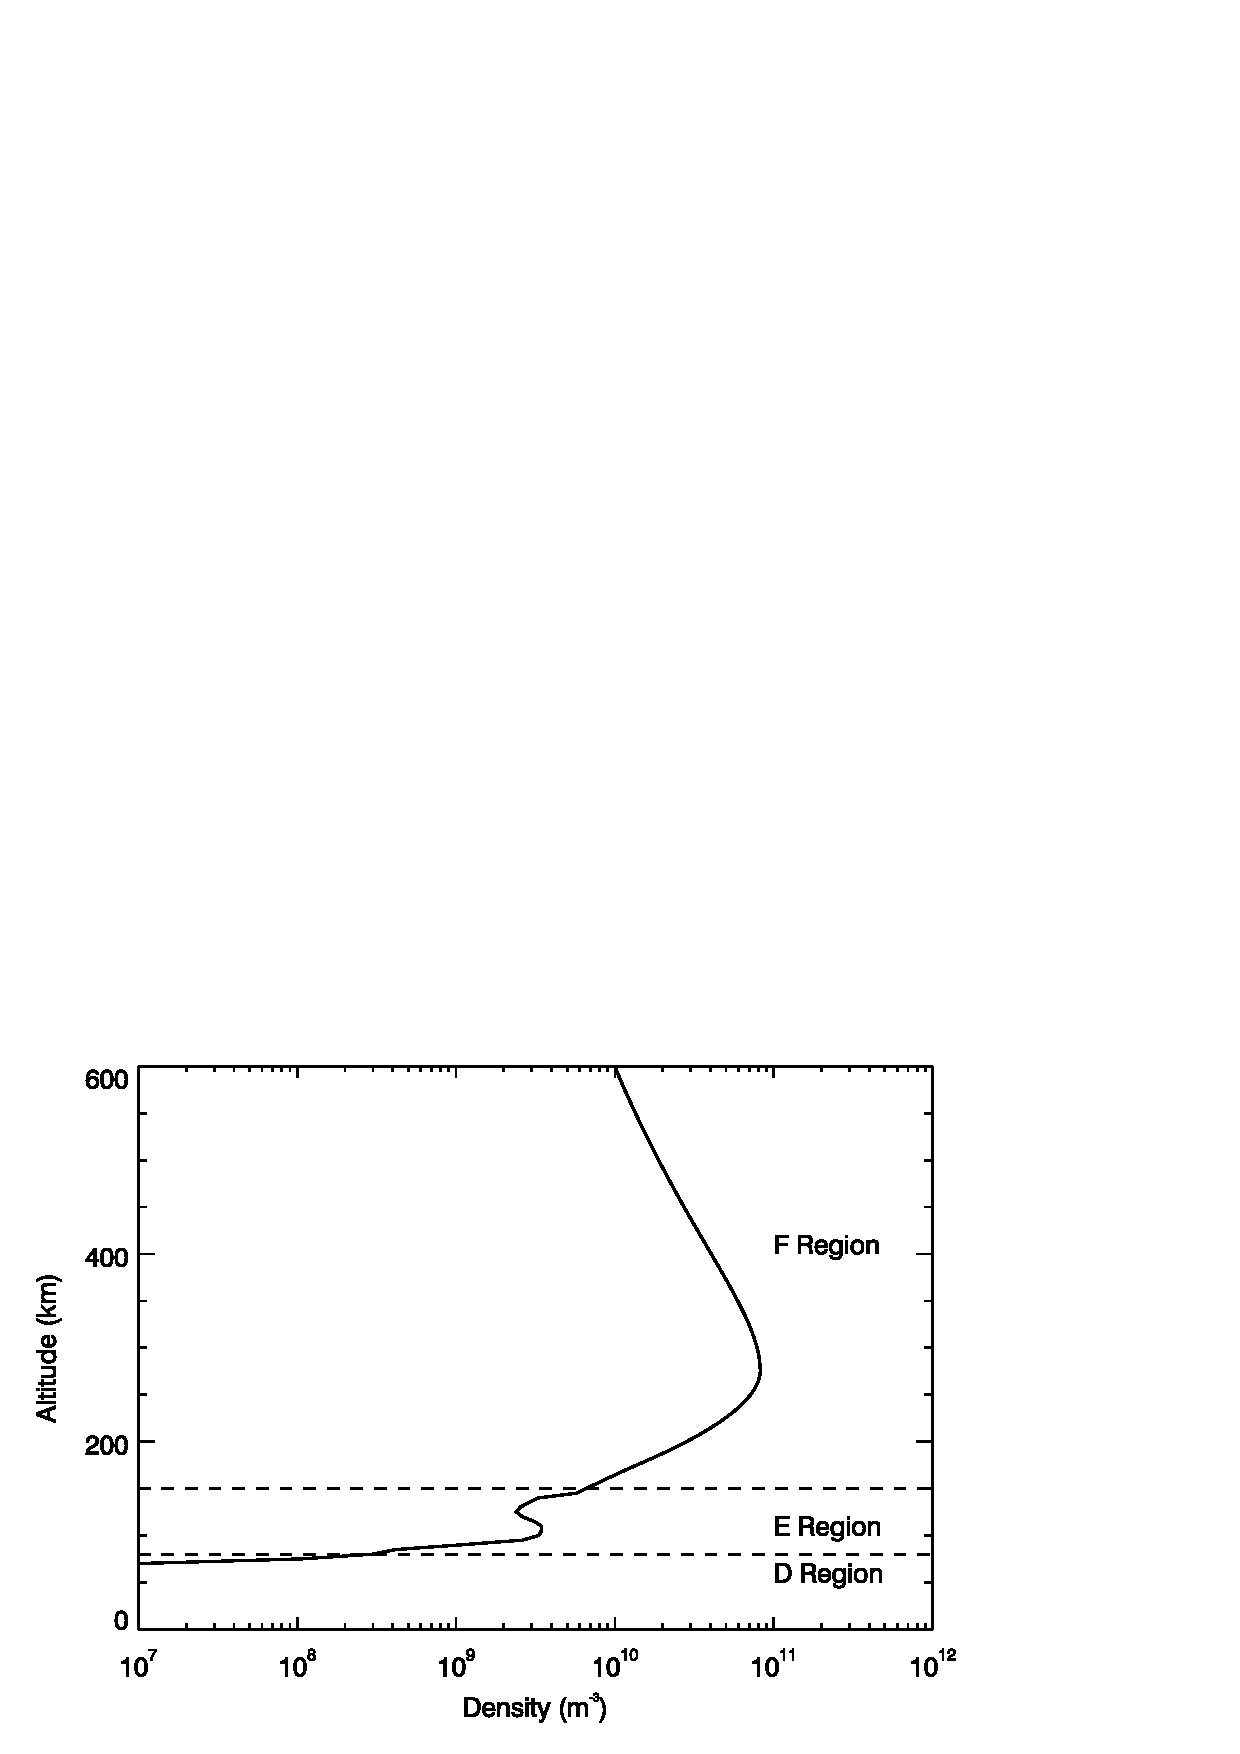
\includegraphics[width=\textwidth]{densprofile.pdf}
	\caption{Altitude profile of electron density throughout the ionosphere found from the IRI model.  Typical ranges of the \(D\), \(E\), and \(F\) regions are identified.}
	\label{fig:densprofile}
\end{figure}

Above 50 km, the primary neutral particles are atomic oxygen, O, molecular oxygen, O\(_2\), and molecular nitrogen, N\(_2\).  Common ions at these altitudes are therefore mostly composed of oxygen and nitrogen, O\(^+\), NO\(^+\), O\(_2^+\), N\(_2^+\), but hydrogen, H\(^+\), can contribute as well, particularly at higher altitudes \citep{Kelley2009}.  In the ionosphere, neutral densties are typically several orders of magnitude higher than ion densities, however even a small number of charged particles changes the behavior of the region dramatically.  Because there are so many different ion species, plasma density is usually discussed simply in terms of electron density.  Plasmas are assumed to be quasineutral, meaning that electron and ion densities are approximately the same so the plasma does not have an overall charge.  The electron density is equal to the sum of densities of all the ions in the plasma, or \(n = n_e = \sum n_i\).

\subsection{Ionospheric Regions}
\label{sec:ionosphere_regions}
The ionosphere is typically divided into three regions, Figure \ref{fig:densprofile}.  The D region is located between 80 and 90 km in altitude and typically only exists in the daytime when the ionosphere is sunlit.  The E region typically exists between 90 and 130 km with a density peak between 105 and 110 km, depending on factors such as time of day and season.  Above 130 km is considered to be the F region, which has a density peak around 250 km, Figure \ref{fig:densprofile} \citet{Luhmann1995}.  The F region can actually have two peaks under some daytime conditions, notated as the F1 peak and the F2 peak.  The peak heights and densities of each of these regions is highly variable both diurnally and seasonally.  In Figure \ref{fig:densprofile}, the daytime profile is shown with the solid line next to a nighttime profile with a dashed line.  Note that night electron densities are lower at all altitudes due to the lack of photoionization during nighttimes.  In addition, the F-region peak moves to higher altitudes at night.  The focus of this thesis will be the F region.

Because the concentrations of ions and neutral particles changes with altitude, each of these regions have distinct plasma physical properties that make them unique.  The main issue is whether the the large-scale motion of a particle is controlled more by the magnetic field (the particle is magnetized) or by collisions with other particles (the particle is collisional).  This can be determined by comparing the collision frequency, \(\nu_\alpha\), to the gyrofrequency, \(\Omega_\alpha\), of a particular species, where \(\alpha\) corresponds to either electrons, \(e\), or ions, \(i\).  If \(\Omega_\alpha \gg \nu_\alpha\), the particle completes many gyrations between each collision, so its motion is determined mostly by the magnetic field and it is magnetized.  If \(\nu_\alpha \gg \Omega_\alpha\), the particle collides with other particles much more often than it complete a gyration, so it is considered collisional.  The gyrofrequency is dependent on the mass and charge of the particle and the strength of the magnetic field, \(\Omega_\alpha = q_\alpha B/m_\alpha\), so is roughly constant through the ionosphere because the magnetic field strength does not change much throughout these altitudes.  The collision frequency depends on the density of a species relative to the density of all other species in the plasma and can be calculated from a series of standard expressions \citep{Schunk1980,Schunk2009}.  In the E region, \(\Omega_e \gg \nu_e\), so electrons are magnetized.  However, the motion on ions is dominated by collisions between ions and neutrals (\(\nu_i > \Omega_i\)), so ions in the \(E\) region are considered collisional.  In the \(F\) region where the neutral density is much lower, both ions and electrons are magnetized, \(\Omega_\alpha \gg \nu_\alpha\).  These differences in how charged particles move impact the conductivity and plasma waves development, which is further discussed in Section \ref{sec:lit_theory}.

\subsection{Plasma Structuring in the Polar Ionosphere}
\label{sec:polar_structure}

This thesis is concerned with the polar ionosphere, which is a particularly interesting and dynamic region due to the presence of open field lines to the solar wind.  The main focus of this work will be plasma density perturbations, often called irregularities.  Density irregularities in the polar cap can occur on scales ranging from thousands of kilometers to less than a centimeter \citep{Tsunoda1988}, and a summary of some of these irregularities is presented in Figure \ref{fig:polarirreg}.  Large-scale plasma irregularities are typically considered to be any density structure on the scale of greater than 30 km \citep{Kelley2009}.  Some common examples are polar patches, polar holes, and sun-aligned arcs.  Polar patches are large density enhancements (usually at least twice the background plasma density) that travel across the polar cap with the background convection, Figure \ref{fig:polarirreg} \citep{Weber1984,Valladares1994}.  Polar holes are plasma density depletions that typically occur in the \(F\) region slightly poleward of the auroral oval \citep{Benson2001}.  Sun-aligned arcs are large density forms that stretch across the polar cap along the sun-earth line.  They are very narrow and often characterized by large and complex velocity shears on either side of the arc \citep{Valladares1991}.  Large scale plasma structures and the density gradients that surround them often serve as a platform for smaller-scale structures to form as well.  Polar patches, for instance, are known to form large finger-like structures along their trailing edges, Figure \ref{fig:polarirreg} \citep{Gondarenko2004b,Hosokawa2016}.

\begin{figure}
	\includegraphics[width=0.8\textwidth]{irregularity.pdf}
	\caption{Schematic of different scale size plasma density irregularities that occur in the polar cap.  Polar patches, orange, move with the background ionospheric convection, indicated by green contours.  Field-aligned irregularities, FAIs, are density perturbations that form along the magnetic field lines, pink lines.}
	\label{fig:polarirreg}
\end{figure}

Intermediate-scale plasma irregularities are those ranges from 100 m -- 30 km \citep{Kelley2009}.  These are also referred to as scintillation-causing structures and are responsible for many of the negative space weather effects that are observed on Earth.  One important example of a space weather effect is when the ionosphere changes the phase and amplitude of the original signal, called radio scintillation, which affects the ability of satellites to communicate with ground receivers.  This can cause communication blackouts or introduce large errors into GPS/GNSS (Global Positioning System/Global Navigation Satellite System) calculations, affecting navigation.  Because communication and navigation technology is implemented in both every day civilian life as well as government and military operations, the effects of this kind of signal scintillation can be far reaching.

Small-scale structuring is generally considered to be all irregularities less than 100 m \citep{Kelley2009}.  Although small-scale irregularities are not responsible for scintillation that directly impact GPS/GNSS performance, they can be the easiest to study because of large data sets collected from high frequency ionospheric radars globally for several decades (discussed further in Section \ref{sec:superdarn}).  Because electrons move far more easily along magnetic field lines than across them, density perturbations tend to be aligned with the magnetic field and are often known as field-aligned irregularities (FAI), Figure \ref{fig:polarirreg}.  The irregularity classifications presented here are rough categories only and a high degree of coupling between different scales occurs, which makes plasma structures of all scales (large, intermediate, and small) important for plasma structuring processes.  For instance, large-scale structures such as polar patches may very well have internal intermediate- and/or small-scale structuring.  A turbulent cascade is often assumed to connect these different scales, but because various instruments or techniques usually only observe structuring on a particular scale, it is difficult to find direct evidence of this or how exactly it occurs \citep{Kinter1985,Tsunoda1985}.  A description of some of the particular instruments and models that are used in this thesis follows.

\section{Observational Techniques and Models}

\subsection{Coherent Scatter Radars}
\label{sec:csr}
In this thesis, we make extensive use of Coherent Scatter Radars (CSR), which have been used to study the ionosphere for the last half century.  The radar transmits a radio wave, which can scatter off plasma structures in the ionosphere, and then be detected by the recieving antennas.  The time difference between when the signal was transmitted and when it was detected and the power and phase of the returned signal can then be used to determine characteristics of plasma irregularities.

There are three measurements typically made by CSR systems: backscatter power, line-of-sight (LoS) velocity, and spectral width.  Backscatter power is the power of the returned signal that the radar's recievers detect.  Typically, a threshold is selected for the minimum power acceptable for a return to be considered an actual signal instead of background noise.  LoS velocity is the component of the total plasma drift velocity that is measured along the transmitted signal direction.  Because radars measure velocity through the doppler shift of backscatter, only the component of the velocity vector can be measured.  Spectral width represents the width of the doppler power spectrum and can determine characteristics of irregularities \citep{Greenwald1985}.

CSR systems can operate by transmitting pulses instead of continuously.  This allows the distance between the radar and the target to be found (based on the time difference between when the pulse is transmitted and received).  The size of the range gate is determined by the length of a radar pulse, Equation \ref{eqn:range_gate}.\
\begin{equation}
	\label{eqn:range_gate}
	\Delta r = \frac{c\Delta t}{2}
\end{equation}.
Here, \(\Delta r\) is the size of a range gate, \(\Delta t\) is the pulse length, and \(c\) is the speed of light.  Longer pulses result in larger range gates, resulting in poorer spatial resolution.

When the radar transmits continuously, backscatter will be received, but because it is impossible to know when that signal was transmitted, the difference in time between transmission and receiving cannot be used to calculate how far away the backscatter volume is.  Conversly, if the radar only transmits a pulse of a certain length of a certain length and then ``listens'' for its return, the time between transmission and return is known and the distance the pulse traveled can be calculated and therefore the location of the backscattering volume \citep{Farley1972,Greenwald1983}.  However, using this simple single-pulse method another pulse cannot be transmitted until the first pulse returns, limiting the temporal resolution that can be achieved.  This can be improved by using a multipulse scheme, which will be discussed below \citep{Farley1972,Greenwald1983,Greenwald1985}.

A short time between pulse returns is necessary to allow Doppler velocities to be calculated, particularly at long ranges.  The maximum Doppler shifted frequency that can be observed by a radar is the Nyquist frequency, \(f_n\), which is equivilent to half the sampling frequency, \(f_s\), Equation \ref{eqn:nyquist}
\begin{equation}	
	\label{eqn:nyquist}
	f_n = \frac{f_s}{2}
\end{equation}.
Radars operating in single-pulse mode must have a very low sampling frequency, as described above, particularly at long ranges where the pulse must travel a long distance.  This severely limits the Doppler shift that can be measured, which places an upper limit on the LoS Doppler velocity that can be calculated with this technique.  For an ionospheric radar observing a structure 2000 km away, it would take about 13 ms for a signal traveling at the speed of light to travel to the the structure and back to the radar, wich corresponds to a sampling frequency of \(f_s = 75\) Hz.  The Nyquist frequency is then \(f_n = 37.5\) Hz, which corresponds to a maximum measurable Doppler velocity of \(\sim550\) m/s.  Flows in the ionosphere have been known to exceed 1000--2000 m/s, so single pulse sampling is insufficient for these purposes.

Instead of waiting for each individual signal to be recieved before transmitting the next, ionospheric radars typically employ a multipulse mode. In a multipulse mode, the radar transmits a series of pules with different time intervals or lags between them.  This can introduce complications when backscatter from different pulses at different ranges is received by the radar at the same time, referred to as cross-range interference, but these effects can be mitigated using correlation techniques \citep{Farley1972}.  The smallest lag between two pulses is known as the multi-pulse increment, \(\tau\).  All other lags are integer multiples of \(\tau\), which allows the calculation of the corresponding lags of the complex autocorrelation function (ACF).  The ACF is used to find the spectral characteristics of the backscatter, from which the LoS velocity, spectral width, and backscatter power can be obtained.  Overall, multi-pulse techniques are generally considered far more appropriate for ionospheric studies than single pulse techniques \citep{Farley1972,Greenwald1983,Greenwald1985,Barthes1998,Ponomarenko2006}.

The first observations of the ionosphere by CSRs were made in the 1930s \citep{Eckersley1937,Harang1938}.  Over the next several decades, numerous used ground-based radars to advance our understanding of the ionosphere and radio aurora \citep{Hultqvist1964,Leadabrand1965,LangeHesse1967,Unwin1972,Sahr1996}.  In the 1970s and 1980s, the Scandanavian Twin Auroral Radar Experiment (STARE) produced the first continuous large data-set, similar to how modern CSR systems are run.  STARE consisted of two very high frequency (VHF) radars with overlapping FoVs that were designed to measure FAIs in the \(E\) region of the ionosphere \citep{Greenwald1997}.  The advantage of two radars with overlaping FoVs was the ability to observe the same structures from two different directions.  Because each radar can only measure the LoS velocity of a structure, two simultanious observations from different directions allows two different velocity vecotor compontents to be found, and hense the total velocity vector can be calculated.  This technique is still commonly used with CSR system.

\subsubsection{Super Dual Auroral Radar Network (SuperDARN)}
\label{sec:superdarn}
The primary instruments used within this body of work are radars within the Super Dual Auroral Radar Network (SuperDARN), a global network of high frequncy (HF) CSRs that was designed to measure small-scale plasma structures in the ionosphere and map the global plasma convection.  The network currently consists of about 35 operational radars between the northern and southern hemispheres distributed at mid-, high-, and polar latitudes, Figure \ref{fig:superdarnmap}.  After the STARE experiment \citep{Greenwald1978}, the first HF ionospheric radar was built in Goose Bay, Canada in 1983, which would become the first of the SuperDARN radars \citep{Greenwald1985}.  

\begin{figure}
	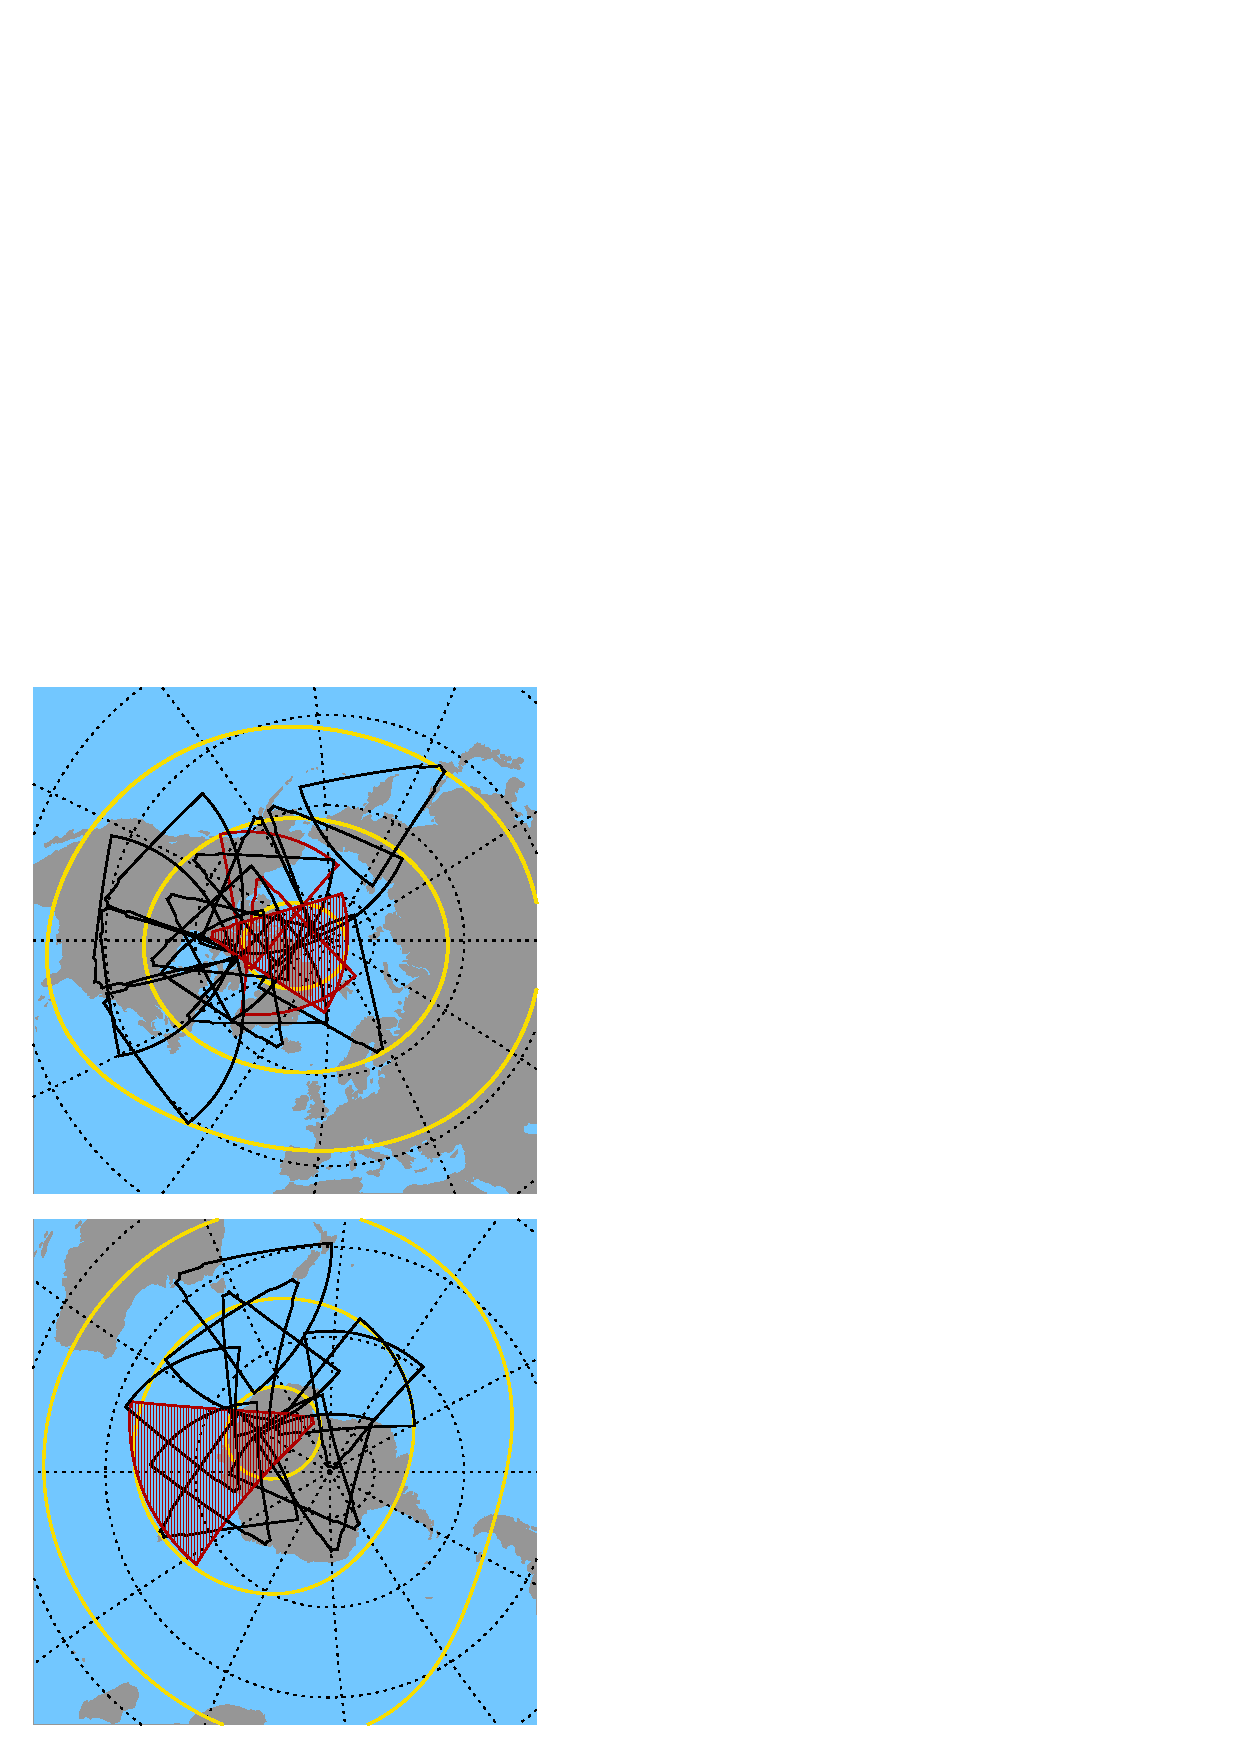
\includegraphics[width=\textwidth,angle=180]{SuperDARNmap.pdf}
	\caption{FoVs of all operational SuperDARN radars in both the northern (left) and southern (right) hemispheres.  Polar latitude radars are shown with the red outlines.  The radars at Rankin Inlet (northern hemisphere) and McMurdo Station (southern hemisphere) are shaded in red because these two instruments are particularly important in the following studies.  Lines of constant magnetic latitude are shown in yellow at \(\Lambda = 40\deg, 60\deg, 80\deg\) in the northern hemisphere and at \(\Lambda = -40\deg,-60\deg,-80\deg\) in the southern hemisphere.}
	\label{fig:superdarnmap}
\end{figure}

It is necessary to use HF radars to study ionsospheric structures in the polar cap because the magnetic field is close to vertical and in order for the radar beam to meet the perpendicularity condition to observe FAIs, the beam must be refracted through a dense ionosphere.  VHF radar beams are not refracted enough in the polar cap and the beam will pass through the ionosphere without FAIs producing backscatter.  SuperDARN radars operate nominally between 8--20 MHz, which, according to the Bragg scatter equation for backscatter, corresponds to observing decameter-scale plasma waves.  Each radar consists of 16 independent antennas that transmit a radio wave and receive backscatter from the ionosphere.  Beams are electronically steerable and most radars have between 16 and 24 beams in normal operation mode, each beam being \(3.25\deg\) in azimuth.  Each beam consists of 75--100 range gates, which are generally either 15 km or 45 km in length \citep{Chisham2007}.  SuperDARN radars were originally designed to used a 7 pulse ACF \citep{Farley1972,Greenwald1983,Greenwald1985}, however since 2011, most radars have begun using an 8 pulse sequence.   The multi-pulse increment, \(\tau\), is 2400 \(\mu\)s, which corresponds to a Nyquist frequency of about 200 Hz, small enough to measure plasma drift velocities up to 3000 m/s.  The spectral characteristics of backscatter are derived from the ACF using the FITACF algorithm \citep{Ponomarenko2006}.

One of the original purposes of SuperDARN was to produce maps of the plasma convection patterns in the polar caps using 2D velocity vectors.  Originally this was accomplished by considering two radars with overlapping FoVs.  If both recieved backscatter from the same scattering volume, two LoS velocities could be found for that scattering volume, which could be combined to find a 2D velocity vector \citep{Ruohoniemi1989}.  The modern method for creating convection maps involves taking all data recorded by all radars in a particular hemisphere and finding the best fit to a 2D ionospheric electrostatic potential using Legendre functions \citep{Ruohoniemi1998}.  For convection maps, only data from the \(F\) region is considered.  If there is not enough velocity data to confine the fit sufficiently, the measured data points are supplemented with a statistical model based on solar wind IMF conditions \citep{Ruohoniemi1995,Ruohoniemi2005}.

Because convection maps require data covering as wide a range of magnetic local time sectors as possible, SuperDARN radars are continuously operational, usually in a common mode.  This creates a vast database of high-quality measurements of small-scale FAIs, which is very useful for other studies on irregularity occurrence and plasma structuring.  In the studies presented here, data was primarily used from the SuperDARN radars located at Rankin Inlet, Canada (RKN) and McMurdo Station, Antarctica (MCM).  These two radars have been shaded in Figure \ref{fig:superdarnmap}.  MCM is the only polar radar in the southern hemisphere.  Although the FoVs of other radars cover parts of the polar cap, they only to at either E region ranges or the furthest of the F region ranges, for which there is rarely much backscatter.  There are currently three polar radars in the northern polar cap, but the FoV of RKN overlaps the Resolute Bay Incoherent Scatter Radar FoV (discussed in Section \ref{sec:isr}, which makes it particularly useful for multi-instrument studies of the ionosphere.

\subsection{Incoherent Scatter Radar}
\label{sec:isr}
Similar to CSRs, incoherent scatter radars (ISRs) are ground based radars that are used to probe the ionosphere.  However, they use a fundamentally different technique to observe structuring, which allows them to measure bulk plasma parameters in contrast to small-scale irregularity characteristics.  While CSRs receive backscatter from relatively large, ``coherent'' density structures in the ionosphere, ISRs operate by radar scattering from waves due to the random thermal motion of electrons in the plasma.  The radar receivers then measure a spectrum of frequencies with different power \citep{Gordon1958}.

The scattering cross section for a volume of N electrons in the ionosphere is given by \(\sigma_n = N \sigma_e\) for radio waves with a wavelength small compared to the Debye length of the plasma, where \(\sigma_e\) is the scattering cross section of a single electron \citep{Gordon1958,Fejer1960}.  The relationship to the plasma Debye length is important because at scale sizes smaller than the Debye length, the plasma is not capable of organized motion, so the motion of the elections is only due to their own thermal energy and not larger scale plasma waves.  The signal returned from this kind of scatter was postulated to have a very low power and a very broad spectral width, however after the first ISR was built, the spectrum was found to be much narrower than previously expected \citep{Evans1969}.  This can be attributed to the effect that the much slower ions have on free electrons in the plasma through ion acoustic waves \citep{Bowles1958}.  The practical results of this is that ISRs can use radio waves of a much longer wavelength than originally anticipated, on the order of \(\sim\)1 m.

Analysis of the returned power spectrum reveals the electron density, electron and ion temperatures, and LoS ion velocity \citep{Evans1969,Rishbeth1985,Nicolls2007a}.  Using a model of chemical composition at different altitudes, the average ion mass can also be found.  In addition, 3D convection velocities and electric field vectors can be derived from LoS ion velocity measurements in some of the more modern ISRs by assuming both \(\vec{E}\) and \(\vec{V}_E\) are constant across the radar's FoV \citep{Heinselman2008}.  More recently, a new algorithm has been developed that used the Lagrange method of undetermined multipliers to generate 3D convection velocity and electric field vectors without making this limiting assumption \citep{Nicolls2014}.  Each instrument must be calibrated with known electron density measurements to account for noise and system constants \citep{Nicolls2007a}.  This is done using the plasma frequency measured from either the plasma line of the ISR spectra during summer daytime period or ionosonde measurements for all other times \citep{Bahcivan2010,Themens2014}.

\begin{figure}
	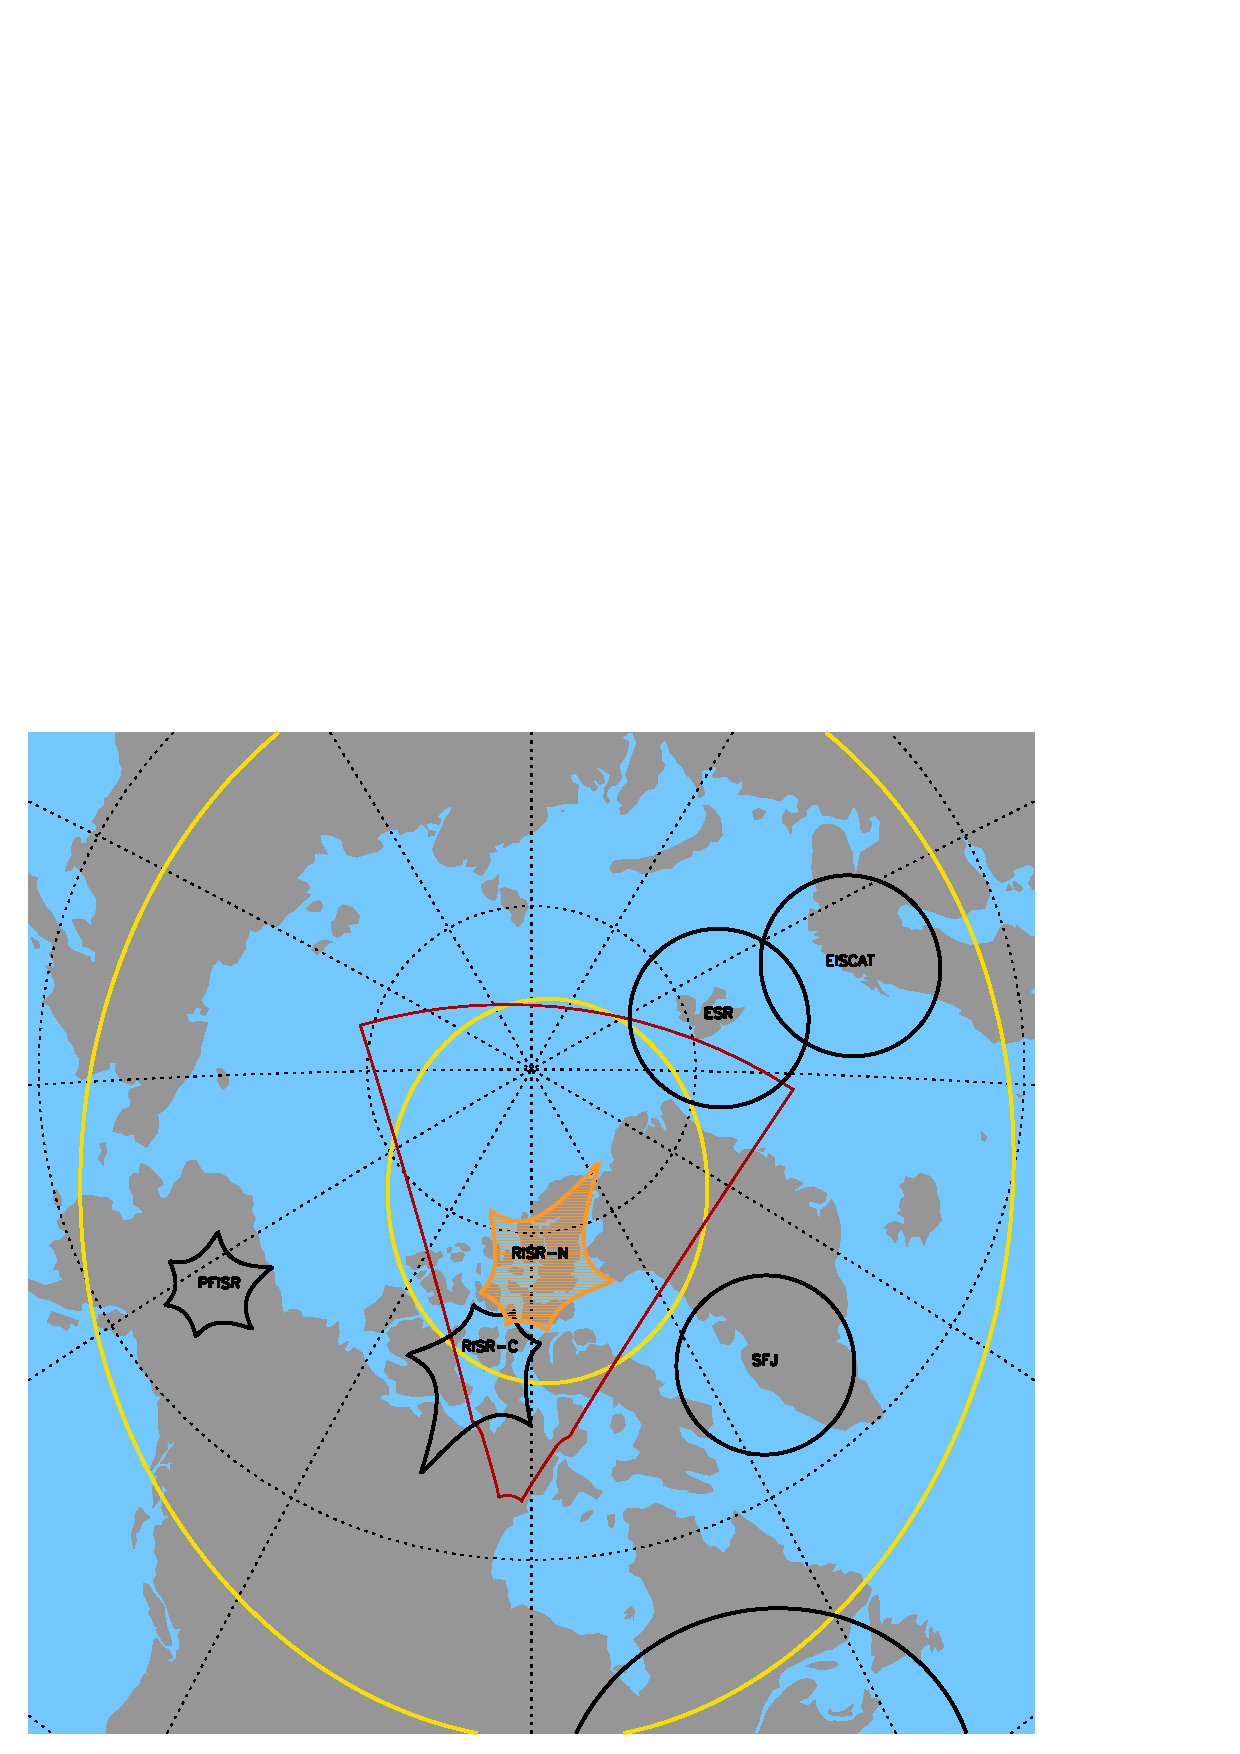
\includegraphics[width=\textwidth]{ISRmap.pdf}
	\caption{FoVs of all ISRs in the northern polar region.  The individual radars shown are identified by their commonly used acronyms: Poker Flat (PFISR), Resolute Bay North (RISR-N), Resolute Bay Canada (RISR-C), Sondrostrom (SFJ).  RISR-N, which is primarially used throughout this thesis, is shown in orange.  The FoV of the RKN SuperDARN radar is shown by the red outline.  Lines of constant MLAT are shown at \(\Lambda=80\deg,60\deg\) in yellow.}
	\label{fig:isrmap}
\end{figure}

The first ISR was built in Arecibo, Puerto Rico in the 1950s \citep{Gordon1958}.  Since then, at least 8 other ISRs have been deployed around the world at equitoral, mid-, and high-latitudes.  A map of the ISR systems currently operational in the northern polar cap is shown in Figure \ref{fig:isrmap}.  The most recent advancement has been the development of Advanced Modular Incoherent Scatter Radars (AMISR), of which there are currently three in use, one at the Poker Flat Rocket Range (PFISR), just north of Fairbanks, Alaska and two in Resolute Bay, Canada (RISR-N and RISR-C).  The advantage of these new systems is that they are electronical steerable, unlike older ISRs which consisted of a large dish that had to be physically moved to change the beam direction.  This allows beams to be transmitted in many different directions at a very high time cadence, giving the radar the capability to make measurements in multiple directions almost simultaneously \citep{Nicolls2007a,Nicolls2007b,Bahcivan2010}.  This is very important for creating 2D maps of ionospheric conditions and tracking how they change in time \citep{Semeter2009,Dahlgren2012a,Dahlgren2012b}.

AMISR systems typically have two types of pulses, a long pulse (LP) with 72 km range gates for \(F\)-region studies and an alternating code pulse (AC) with 4.5 km range gates gates for \(E\)-region studies.  The exact number and configuration of beams depends on the radar mode used and can be changed easily due to the system's electronic steering.  In the common WorldDay mode, there are typically 11 beams and data is collected at \(\sim\)1 min intervals, although this can change slightly between different renditions of the WorldDay mode.  WorldDay mode creates the characteristic star shaped FoV seen in Figure \ref{fig:isrmap}

One of the most important advantages of ISR systems over CSRs is the ability to directly measure electron density in the ionosphere.  However, because ISRs are much scarcer and are only typically run on in WorldDay mode a few days out of every month, data are not as widely available.  In addition, ISRs do not actually observe small-scale coherent plasma structures like the SuperDARN HF network does.  However, they can directly measure large-scale structures and image density variations on scales larger that 100 km (limited by the number of beams and range gate size).  For these region, it is often useful use a combination of CSR and ISR measurements in ionospheric plasma structuring studies, when possible.  The primary ISR used in the present volume of work is the north face of the AMISR system at Resolute Bay, Canada, RISR-N, shown in orange in Figure \ref{fig:isrmap}.  The FoV of RISR-N overlaps that of the RKN SuperDARN radar, red outline in Figure \ref{fig:isrmap}, making it ideal for these types of comparison studies, Chapters \ref{sec:paper1} and \ref{sec:paper3}.

\subsection{IRI Model}
\label{sec:iri}
In addition to radars, models can be a useful tool for understanding the background conditions in the ionosphere, particular in regions where there is poor instrumental coverage.  The International Reference Ionosphere (IRI) is an empirical model of the Earth's ionosphere.  It was originally created in 1969 as a joint effort between the Committee on Space Research (COSPAR) and the International Union of Radio Science (URSI) and has been periodically updated since then \citep{Rawer1975,Rawer1978,Rawer1981,Bilitza1985,Bilitza1986,Bilitza1990,Bilitza1997,Bilitza2001,Bilitza2008}.  The current version is IRI-2012 \citep{Bilitza2014}, which is used throughout the work done here.

The IRI model produces outputs of electron density, temperatures of electrons, ions, and neutrals, ion composition (O\(^+\), H\(^+\), He\(^+\), O\(_2^+\), NO\(^+\), N\(^+\)), and total electron content (TEC).  The model requires the input of a location (latitude, longitude, and altitude) and time (year, date, and time).  Additionally, the model gives the option to choose between two F peak models and three bottomside thickness models.  There are a variety of other optional input parameters such as sunspot number, ionospheric index, and F10.7 radio flux which can help make the output parameters more accurate for a particular situation.  Additionally, the model is capable of producing profiles of any of the output parameters in either space or time.  This is particularly significant for height profiles, and allows the peak heights and densities of the \(E\) and \(F\) region to be calculated.

Although the IRI model is very useful for providing background plasma density conditions where no instruments are available to make measurements, it is important to bear in mind that it is a model and therefor only represents the average conditions.  Although it is fairly accurate at mid-latitudes \citep{Coisson2006,Bilitza2012}, it does not necessarily represent variations within the polar cap well \citep{Themens2014,Makarevich2015}.  In particular, the height of the F-region peak tends to be underestimated in daytime and the bottomside thickness does not show realistic seasonal and diurnal variation \citep{Themens2014}.  

Despite this, the IRI model is still a very important tool for establishing a density profile at any time in any location in the ionosphere.  And example of an altitude profile of plasma density provided by the IRI model is shown in Figure \ref{fig:densprofile}.  The displayed profiles shows how the electron density changes with altitude at local noon (day) and midnight (night) on January 1, 2007 at \(75\deg\) N, \(0\deg\) E, geographic.

One of the most important uses of the IRI model has been its integration into ray tracing simulations.  Throughout this work, it is valuable to determine the degree to which HF radar beams refract through a dense ionosphere.  This can be done through standard raytracing tools based on numerical solutions to the Hamiltonian raypath equations, as shown in Chapter \ref{sec:paper1} \citep{Haselgrove1963,Jones1975}, however these tools require a 2D density profile along the path that the radar beam travels.  It is possible to assume a Gaussian distribution or Chapman layer as a simple model of the F-region peak, but it is much more instructive to use output from the IRI model, as is done in this work, as it is sensitive to changes in latitude as well as seasonal and diurnal variations.

\section{A Brief Review of Plasma Structuring Theory and Observations in the Polar Cap}
Much work has been done over the past several decades to study the complicated picture of plasma structuring in the polar cap, including theoretical analysis of plasma dispersion relations, simulations of plasma dynamics, and observations of plasma structuring using a variety of instruments.  Here, a survey will be given of some of these advancements and the current state of understanding plasma structring on a range of scales.

\subsection{Polar Patch Formation}
\label{sec:lit_patches}
Large-scale structuring in the polar cap can take a variety of forms, Section \ref{sec:polar_structure}, but here we will focus on large regions of enhanced plasma density known as polar patches  \citep[e.g.][]{Weber1984,Weber1986,Buchau1983,Buchau1985}.  One of the primary interests of this thesis is the relationships between irregularities of different scales and small-scale structuring has long been observed around polar patches \citep{Weber1984,Milan2002b,Moen2012}.  Although small-scale structures have also been observed around sun-aligned arcs \citep[e.g.][]{Koustov2012}, these structures also tend to be more complicated and often are surrounded by intense shears and electric fields \citep{Safargaleev2000,Aikio2002,Kozlovsky2007}.  Additionally, polar patches occur relatively frequently, providing a good opportunity to study irregularity coupling at different scales \citep{Rodger1996}.  In theory, many of the results presented in this work pertaining to the strong gradients on the edges of patches could also easily be applied to the edges of polar holes, but to date, far less attention has been paid to polar holes in the literature, making it challenging to accurately put observations in context \citep{Makarevich2015}.

The first observations of polar patches were made in the 1960s by \citet{Hill1963}.  They can range in size from 100 km up to 1500 km in diameter and can have peak densities as much as eight times that of the background ionospheric plasma \citep{Weber1986,Hosokawa2014}.  Polar patches are know to emerge on the dayside and then propagate with the background plasma convection across the polar cap to the nightside, where they either disintegrate or recombine with enhanced-density plasma in the auroral oval \citep{Weber1985,Weber1986}.

There have been at least 6 mechanisms proposed for how polar patches form on the dayside \citep{Crowley1996,Carlson2012}:
\begin{enumerate}
	\item Discrete changes in solar wind parameters, usch as IMF, density, speed, and pressure \citep{Sojka1994}
	\item Average flow patterns varying in time \citep{Anderson1988}
	\item Transient magnetopause reconnection \citep{Lockwood1992b}
	\item Plasma production by cusp particle precipitation \citep{Rodger1994,Millward1999}
	\item Plasma flow jet channels that cut continuous streaches of plasma into segments 	\citep{Valladares1998}
	\item Alfven wave coupling \citep{Prikryl1999}
\end{enumerate}.
Although particle precipitation has been shown to create enhanced plasma density in the cusp region \citep{Rodger1994}, it is unreasonable for this mechanism to account for the largest density enhancements observed in polar patches.  These high densities must originate from the reservoir of solar illuminated plasma on the dayside.  Additionally, a mechanism is still required to separate patches from the cusp region.  High speed flow channels can ``cut'' segments off of a tongue of high-density plasma that has been pulled into the polar cap by convection \citep{Valladares1994,Valladares1998}.  Models have also shown that changing large scale convection patterns quickly in time does produce density structures similar to patches \citep{Anderson1988}.  However, the mechanism that seems to be dominant for the majority of polar patches observed is transient magnetic reconnection \citep{Carlson2012}.

In order to discuss patch formation by transient magnetic reconnection, it is important to first understand the steady-state ionospheric convection patterns in the polar cap and how they relate to the magnetosphere \citep{Cowley1980}.  Figure \ref{fig:magnetosphere} is a schematic of how the IMF, magnetosphere, and ionospheric polar cap are all interconnected.  In general, magnetic field lines in the magnetosphere can either be closed (grey lines in Figure \ref{fig:magnetosphere}), meaning they connect only the north and south pole of the Earth, or open (light blue lines in Figure \ref{fig:magnetosphere}), when one of the ends of the field lines originates from the sun such that the field line is connected directly to the IMF.  IMF lines that are not connected to the Earth are shown in dark blue in figure \ref{fig:magnetosphere}.  The polar cap boundary is generally defined as the border between open and closed magnetic field lines, shown by the green line in Figure \ref{fig:magnetosphere}.

By Faraday's Law, the total electromotive force, \(\xi\) around the polar cap boundary is equal to the rate of change of magnetic flux, \(\Phi_B\) within the polar cap, Equation \ref{eqn:pc_imf} \citep{Lockwood1992a}.  In steady-state solutions, \(d\Phi_B/dt = 0\), so \(\xi=0\) by definition, however the polar cap is known to be a highly dynamic system, so changes in magnetic flux are expected.
\begin{equation}
	\label{eqn:pc_imf}
	-\xi = \frac{d\Phi_B}{dt} = B\frac{dA_{pc}}{dt}
\end{equation}
In the polar cap at ionospheric altitudes, the magnetic field strength is relatively constant at around \(5\times 10^-5\) T, so any changes in magnetic flux must be due to changes in the polar cap area, \(A_{pc}\) due to the polar cap boundary expanding or contracting \citep{Lockwood1992a}.  The polar cap boundary changes in response to magnetic reconnection between the magnetosphere and the IMF  on both the day and night sides changing the amount of open magnetic flux.


\begin{figure}
	\includegraphics[width=0.75\textwidth,angle=270]{magnetosphere.pdf}
	\caption{Diagram of the interactions between the IMF, magnetosphere, and polar cap ionosphere.  Closed field lines in the Earth's magnetosphere are shown in grey while open field lines are light blue.  The polar cap open-closed boundary is in green.  Magnetic field lines that are part of the IMF are shown in dark blue.  Magnetic reconnection occurs along the X-line (red) on the dayside of the magnetopause (dashed line).  The X-line can be mapped back along magnetic field lines (orange) to the ionosphere, where their projection is the merging gap (pink dotted line).  During reconnection events, the open-closed boundary expands equatorwards as more open field lines are formed and there is plasma flow across the merging gap.}
	\label{fig:magnetosphere}
\end{figure}

Magnetic reconnection between the IMF and the Earth's magnetosphere occurs along the X-line on the dayside magnetopause (red line in Figure \ref{fig:magnetosphere}).  The X-line in the magnetopause can be mapped along the magnetic field lines (orange) to the ionosphere, where it is referred to as the merging gap (pink dotted line in figure \ref{fig:magnetosphere}) and lies along the steady state polar cap boundary.  

During reconnection events, the polar cap boundary moves equatorward as the open magnetic flux into the polar cap increases, Figure \ref{fig:magnetosphere} \citep{Cowley1991,Lockwood1992a}.  In addition, the potential along the X-line also gets mapped to the merging gap, assuming there is minimal drop in potential along the magnetic field lines \citep{Lockwood1992b}.  The combination of these two effects results in flux being transferred across the boundary at a rate equal to the applied voltage  along the X-line and hence plasma flow across the merging gap \citep{Lockwood1992b}, which will be examined further in Figure \ref{fig:patch_formation}.  

Figure \ref{fig:patch_formation} is a schematic of polar patches being formed through transient magnetopause reconnection.  In all panels, the dayside is the top of the figure and the green line shows the open-closed polar cap boundary, similar to Figure \ref{fig:magnetosphere}.  Plasma flow contours are shown in black and the light orange region represents high density from the dayside reservoir.  The reconnection burst starts at Figure \ref{fig:patch_formation}a and the increasing amount of open magnetic flux moves the dayside open-closed boundary equatorwards, as described above \citep{Cowley1991}.

As reconnection continues in Figure \ref{fig:patch_formation}b, the open-closed boundary continues to expand equatorwards as more open flux is produced, which excites a convection pattern in the polar cap \citep{Cowley1991}.  Simultaneously, this convection starts to transport dense dayside plasma polewards \citep{Lockwood1992b}.  As more open flux is produced, Figure \ref{fig:patch_formation}c, the strength of the plasma flow increases and a large blob of dense, dayside plasma is pulled into the polar cap \citep{Lockwood1992b}.

At Figure \ref{fig:patch_formation}d, the burst of reconnection stops and the open-closed boundary begins to relax polewards \citep{Cowley1991}.  As it moves, it pulls the blob of dense plasma within the polar cap with it, separating it from the reservoir on the dayside \citep{Lockwood1992b}.  Before the convection flow stops completely, Figure \ref{fig:patch_formation}e, the blob of dense plasma ``pinches off'' from the dayside plasma to become an independant patch \citep{Lockwood1992b}.  The exact mechanism by which this happens is not well understood, but it is thought to be related to small variations in the IMF By component shifting the convection pattern slightly \citep{Cowley1980,Lockwood1992b}.  By Figure \ref{fig:patch_formation}f, the open-closed boundary has returned completely to its original position and there is a newly formed patch within in the polar cap.  The process can now repeat to form another patch within the polar cap.

A series of reconnection bursts can create a line of patches all propagating across the polar cap.  Reconnection bursts typically last about 2 minutes with anywhere between 7 and 25 minutes beween bursts \citep{Foster1984,Etemadi1988,Lockwood1992b}.  However, observations have shown convection flow to be close to continuous for much longer periods.  This can be explained by each reconnection burst exciting flow for a much longer interval than the time between bursts.  In this way, a reconnection burst can excite plasma flow before the convection from the previous burst has stopped, and a series of overlapping reconnection events like this can create continuous plasma flow through the polar cap \citep{Cowley1991}. 

\begin{figure}
	\includegraphics[width=0.75\textwidth,angle=270]{patch_formation.pdf}
	\caption{Polar patch formation through transient magnetopause reconnection.  The open-closed boundary is the green line.  Black contours represent plasma flow.  Dense daytime plasma is shown by the orange regions.  The burst of reconnection is occurring in Figures \ref{fig:patch_formation}a--\ref{fig:patch_formation}c but stops in Figures \ref{fig:patch_formation}d--\ref{fig:patch_formation}f.}
	\label{fig:patch_formation}
\end{figure}

\subsection{Theory of Plasma Instabilities}
\label{sec:lit_instabilities}
Plasma structuring, especially at smaller scales, is often discussed in terms of the growth or damping of plasma waves, or instabilities.  As discussed previously in Section \ref{sec:ionosphere_regions}, the plasma characteristics change with altitude in the ionosphere, which causes a variety of different instability mechanisms to be operational depending on the region considered.  The Farley-Buneman instability (FBI), or the modified two-stream instability tends to be a major factor in the \(E\) region where ion inertial effects are strong \citep{Farley1963,Buneman1963}.  Also operational in the \(E\) region but more dominant at higher altitudes is the gradient-drift instability (GDI) \citep{Simon1963,Hoh1963,Linson1970}.  If a wave has a component along the magnetic filed line, the current-conductive instability (CCI) can be operational even if GDI is not \citep{Hoh1960,Ossakow1979,Chaturvedi1981}.  Additionally instability mechanisms emerge if shears are considered, when \(\nabla E \neq 0\), such as the Kelvin-Helmholtz instability (KHI) \citep{Kintner1977,DAngelo1965}.

In the polar F-region ionosphere, GDI is typically considered the dominant structuring process \citep{Weber1984,Cerisier1985,Basu1988,Tsunoda1988}.  GDI is operational when high-density purturbations in the plasma move to regions of lower background density and low-density purturbations in the plasma move to regions of higher background density, such that the wave amplitude grows relative to background conditions.  As plasma drifts and carries irregularities with it, electrons and ions have slightly different drifts and create a perturbed electric field.  This perturbed electric field combined with the background magnetic field causes the density perturbations to \(\vec{E}\times\vec{B}\) drift.  If the drift causes high and low density perturbations to move as desribed above, the instability is operational and the perturbations grow.  If instead high density perturbations drift into regions of higher background density and low density perturbations drift into regions of lower background density, the wave is damped.

Some of the first 1D investigations of the linear GDI growth rate found that it can be described by a simple expression involving the plasma drift speed, \(V_E = |\vec{E}\times\vec{B}|/B^2\), and the gradient scale length, \(L^{-1} = |(\partial n/\partial x)/n|\), Equation \ref{eqn:gdi_old} \citep{Simon1963,Hoh1963,Linson1970}
\begin{equation}
	\label{eqn:gdi_old}
	\gamma = \frac{V_E}{L}
\end{equation}.
This expression is technically only valid if the density gradient, \(\nabla n\), is in the same direction as the plasma drift velocity, \(\vec{V}_E\), and the wave is propagating perpendicular to both.  A more general expression that is used less often, Equation \ref{eqn:gdi_80s}, does consider an arbitrary wavevector, \(\vec{k}\), but still assumes density gradients parallel to the plasma drift \citep{Tsunoda1988}
\begin{equation}
	\label{eqn:gdi_80s}
	\gamma = \frac{k_y}{k}\frac{\vec{k}\cdot\vec{V}_E}{kL}
\end{equation}.
An even more general consideration involves arbitrary gradient and plasma drift directions \citep{Keskinen1982a,Makarevich2014c}.  In this more general case, the directional dependence of GDI has been shown to be significant, such that the growth rate can actually change signs (determining whether wave growth or damping occurs) with different wavevector directions, so it is important to consider this factor \citep{Makarevich2014c}.  In addition, these expressions have historically only applicable in a particular altitudinal regime, usually the F region.

Recently, a new expression has been introduced that considers any arbitrary wavevector, density gradient, and altitude within the ionosphere, which allows three electrostatic instabilities, FBI, GDI, and CCI, to be considered with a single dispersion relation \citep{Makarevich2016a}.
\begin{equation}
	\label{eqn:gdi_Mak16}
	(H_i-H_e)\omega = (H_i\vec{V}_{e0}-H_e\vec{V}_{i0})\cdot\vec{k}+(C_i-C_e)H_eH_i
\end{equation}
As before, \(\vec{k}\) is the wavevector, \(\omega\) is the wave frequency, and \(\vec{V}_{\alpha 0}\) is the background velocity of species \(\alpha\).  The other quantities in equation \ref{eqn:gdi_Mak16} are not standard and described below.
\begin{equation}
	H_\alpha = S_\alpha F_\alpha + D_\alpha^{-1} F_\parallel \quad\quad\quad 
	C_\alpha = \frac{T_\alpha}{m_\alpha \Omega_\alpha}
\end{equation}
\begin{equation}
	F_\alpha = i k_\perp^2 D_\alpha + \vec{G}\cdot\vec{k}_\perp D_\alpha + \vec{G}\cdot\vec{k}\times\uvec{b} \quad\quad\quad
	F_\parallel = i k_\parallel^2 + \vec{G}\cdot\vec{k}_\parallel
\end{equation}
\begin{equation}
	S_\alpha = \frac{1}{1+D_\alpha^2} \quad\quad\quad
	D_\alpha = -\frac{i}{\Omega_\alpha}(\omega-\vec{k}\cdot{V}_{\alpha 0})+r_\alpha
\end{equation}
The quantity \(r_\alpha\) is the ratio of the collision frequency to the gyrofrequency of a particular species, given by \(r_\alpha = \nu_\alpha/\Omega_\alpha\).  

By taking certain limiting cases, expressions for the instability growth rate in different region can be derived from Equation \ref{eqn:gdi_Mak16}.  These expressions are sumarized in Table \ref{tab:gdi_exps}.  In addition to the quantities previously described in relation to Equation \ref{eqn:gdi_Mak16}, the following are useful for the expressions in Table \ref{tab:gdi_exps}.
\begin{equation}
\begin{split}
	b = -\frac{\vec{G}\cdot\vec{k}\times\uvec{b}}{k_\perp^2} \quad\quad\quad
	y = \frac{k_\parallel}{k_\perp} \\
	R = \frac{\sigma_H}{\sigma_P} = \frac{D_i+D_e}{1+\Psi} \quad\quad
	\psi = -r_ir_e \quad\quad
	\hat{\psi} = \psi\left(1+\frac{k_\parallel^2}{r_e^2 k_\perp^2}\right) \\
	\vec{V}_d = \vec{V}_{e0}-\vec{V}_{i0} = (r_i-r_e)\left[s_es_i(1+\psi)\left(R\vec{V}_E-\frac{\vec{E}}{B}\right)\right]
\end{split}
\end{equation}

For the purposes of this thesis, the cold plasma limit expression in Table \ref{tab:gdi_exps} is most recent and can be rewritten using the definition of \(b\), Equation \ref{eqn:gdi} \citep{Makarevich2014c,Makarevich2016a}.
\begin{equation}
	\label{eqn:gdi}
	\gamma = \frac{1}{1+\psi}\left(\uvec{k}\cdot\uvec{b}\times\vec{G}\right)\uvec{k}\cdot\left(\frac{\vec{E}}{B}-R\vec{V}_E\right)
\end{equation}
Equation \ref{eqn:gdi} is applicable throughout the \(E\) and lower \(F\) regions.  

%It is useful to express Equation \ref{eqn:gdi_Mak16} in the following equivalent form by defining additional terms.
%\begin{equation}
%	\label{eqn:gdi_Mak16_alt}
%	\left(D_i-D_e\right)\omega = \vec{V}_d\cdot\vec{k}\left(\frac{Z_2}{Z_1}\right) + \left(D_i\vec{V}_{i0}-D_e\vec{V}_{e0}\right)\cdot\vec{k}+(C_i-C_e)k_{\perp}^2\left(\frac{Z_3}{Z_1}\right)
%\end{equation}
%In the \(F\) region where background plasma motion is dominated by electric fields perpendicular to the magnetic field, the differential plasma velocity, \(\vec{V}_d\), can be described as 
%\begin{equation}
%	\label{eqn:gdi_Mak16_Vd}
%	\vec{V}_d = \vec{V}_{e0}-\vec{V}_{i0} = (r_i-r_e)\left[s_es_i(1+\psi)\left(R\vec{V}_E-\frac{\vec{E}}{B}\right)\right]
%\end{equation}
%where, \(s_\alpha = (1+r_\alpha^2)^{-1}\).  Additionally,
%\begin{equation}
%\label{eqn:gdi_Mak16_Z}
%\begin{split}
%	Z_1 = i(1+Y)+a+Rb+ycK \quad\quad\quad 
%	Z_2 = R(i+a)-b \quad\quad\quad\quad\quad\quad\\
%	Z_3 = -\frac{\Psi(i+a)^2}{1+\Psi}-Rb(i+a)+\frac{b^2}{1+\Psi}-iy(y-ic)\left[\left(K+1-\Psi^{-1}\right)(i+a)+Rb\left(1-\Psi^{-1}\right)\right]\\+Ky^2(y-ic)^2
%\end{split}
%\end{equation}
%and
%\begin{equation}
%\begin{split}
%	a& = \frac{\vec{G}\cdot\vec{k}_\perp}{k_\perp^2} \quad\quad\quad
%	b = -\frac{\vec{G}\cdot\vec{k}\times\uvec{b}}{k_\perp^2} \quad\quad\quad
%	c = \frac{\vec{G}\cdot\vec{k}_\parallel}{k_\perp k_\parallel} \\
%	\Psi = -D_iD_e& \quad\quad
%	R = \frac{D_i+D_e}{1+\Psi} \quad\quad
%	y = \frac{k_\parallel}{k_\perp} \quad\quad
%	K = \left(1+\frac{1}{\Psi}\right)\left(1+R^2\right) \quad\quad
%	Y = Ky^2
%\end{split}
%\end{equation}.

%By considering certain limiting cases, an expression that is more relevant to the polar F region specifically can be resolved from Equation \ref{eqn:gdi_Mak16_alt}.  First, assume a cold plasma such that the temperature of both ions and electrons is negligible.  In this case, \(T_\alpha = 0\), so \(C_\alpha = 0\).  Secondly assume all irregularities are perfectly aligned with the magnetic field such that \(k_\parallel = 0\).  This means that \(\vec{k}_\perp = \vec{k}\), \(y=0\), and \(Y=0\).  Finally, consider only low frequencies (\(\omega \ll \Omega_\alpha\)) and long wavelengths (\(\vec{k}\cdot\vec{V}_{\alpha 0} \gg \nu_\alpha\)).  If \(D_\alpha\) is expressed as shown below, it can bee seen that these limits result in the first two terms being negligible such that \(D_\alpha \approx r_\alpha\).
%\begin{equation}
%	D_\alpha = -i\frac{\omega}{\Omega_\alpha} + i\frac{\vec{k}\cdot\vec{V}_{\alpha 0}}{\Omega_\alpha} + \frac{\nu_\alpha}{\Omega_\alpha} \approx \frac{\nu_\alpha}{\Omega_\alpha} = r_\alpha
%\end{equation}
%Equation \ref{eqn:gdi_Mak16_alt} can then be expressed as follows.
%\begin{equation}
%	\label{eqn:gdi_Mak16_Freg}
%	(r_i-r_e)\omega = \vec{V}_d\cdot\vec{k}\left(\frac{Z_2}{Z_1}\right)+(r_i\vec{V}_{i0}-r_e\vec{V}_{e0})
%\end{equation}
%The growth rate, \(\gamma\), is contained within the dispersion relation as \(\omega = \omega_r+i\gamma\), so the imaginary part of Equation \ref{eqn:gdi_Mak16_Freg} must be considered separately.
%\begin{equation}
%	\label{eqn:gdi_Mak16_gam}
%	(r_i-r_e)\gamma = \vec{V}_d\cdot\vec{k}\;\text{Im}\left\{\frac{Z_2}{Z_1}\right\}
%\end{equation}
%The differential plasma drift has been defined previously in Equation \ref{eqn:gdi_Mak16_Vd} but the imaginary component of \(Z_2/Z_1\) must still be identified.  Using the definitions of \(Z_1\) and \(Z_2\) provided in Equation \ref{eqn:gdi_Mak16_Z} and the simplifying assumptions discussed above for the F region,
%\begin{equation}
%	\frac{Z_2}{Z_1} = \frac{R(i+a)-b}{i+a+Rb}
%\end{equation}.
%Multiplying both the numerator and denominator by \(-i+a+Rb\) removes the imaginary component from the denominator.  Additionally the local approximation \(G \ll k_\perp\) is taken, which results in \(a\), \(b\), and \(c\) being small so that any second order terms in these quantities can be neglected.
%\begin{equation}
%	\frac{Z_2}{Z_1} = R+ib(1+R^2)
%\end{equation}
%Using the above result and Equation \ref{eqn:gdi_Mak16_Vd}, Equation \ref{eqn:gdi_Mak16_gam} becomes
%\begin{equation}
%	(r_i-r_e)\gamma = (r_i-r_e)s_es_i\left(1+\psi\right)\left(R\vec{V}_E-\frac{E}{B}\right)\cdot\vec{k}b\left(1+R^2\right)
%\end{equation}
%Recognizing that \(s_es_i\left(1+R^2\right) = (1+\psi)^{-2}\) and \(b = \vec{G}\cdot\vec{k}\times\uvec{b}/k^2 = -\vec{k}\cdot\uvec{b}\times\vec{G}/k^2\) by vector identities, a final expression for the GDI growth rate in the F region can be found, which agrees well with the results of \citet{Makarevich2014c}
%\begin{equation}
%	\label{eqn:gdi}
%	\gamma = \frac{1}{1+\psi}\left(\uvec{k}\cdot\uvec{b}\times\vec{G}\right)\uvec{k}\cdot\left(\frac{\vec{E}}{B}-R\vec{V}_E\right)
%\end{equation}.
%Equation \ref{eqn:gdi} will be critical to the analysis done both in Chapter \ref{sec:paper2} and Chapter \ref{sec:paper3} in this thesis.

\begin{table}
\begin{tabular}{l l}
Limiting Case & Growth Rate, \(\gamma\) \\
\hline
GDI/FBI in \(E\) Region & \(\gamma = \frac{1}{1+\hat{\psi}}\left[\frac{\hat{\psi}}{\nu_i}\left(\left(\frac{\vec{V}_d\cdot \vec{k}}{1+\hat{\psi}}\right)^2-C_s^2 k_\perp^2\right)+\frac{br_i\vec{V}_d\cdot \vec{k}}{1+\hat{\psi}}\right]\) \\
GDI/CCI in \(F\) Region & \(\gamma = -\frac{b}{\psi+y^2}\left[\frac{\psi\vec{k}\cdot\vec{E}_{0\perp}+E_{0\parallel}k_\parallel}{B}\right]+C\left[r_ek_\perp^2-\frac{k_\parallel^2}{r_i}\left(1+\frac{r_i^2}{\psi+y^2}\right)\right]\) \\
Cold Plasma in \(F\) Region & \(\gamma = \frac{b}{1+\psi}\left(R\vec{V}_E-\frac{\vec{E}_{0\perp}}{B}\right)\cdot\vec{k}\) \\
\end{tabular}
\caption{Irregularity growth rates in the ionosphere for three different limiting cases \citep{Makarevich2016a}.}
\label{tab:gdi_exps}
\end{table}

Although linear GDI theory as described predicts clear dependence on wave vector direction \citep{Makarevich2014c}, this theory is only really valid in the long-wavelength limit, \(\vec{k}\cdot\vec{V}_E \ll \nu_\alpha\).  In the \(F\) region, the ion-neutral collision frequency, \(\nu_i\), is about 10 Hz and if the drift speed, \(V_E\), is about 1000 m/s, fluid theory only applies for wavelengths greater than 100 m, larger than the decameter-scale waves that are detected by SuperDARN.  This raises the important question of whether or not the same anisotropy that is predicted by linear GDI theory at larger scales can be expected in small-scale irregularities where nonlinear processes may be important.  This issue has mostly been studied through numerical simulations due to the challenges associated with measuring a high-resolution 2D spectrum experimentally.

The first simulations of GDI were done in the 1970s and successfully reproduced structures developing on the trailing edge of large density gradients \citep{Zabusky1973,Doles1976,Scannapieco1976,Ossakow1975,Ossakow1977}.  Later, 2D simulations were expanded to include magnetosphere-ionosphere coupling, but it was found that this only had a substantial effect for very large-scale structures \citep{Keskinen1990}.  3D simulations were introduced of GDI surrounding a large plasma density enhancement \citep{Guzdar1998} and were later improved by including plasma dynamics parallel to the magnetic field and inertial effects so that secondary KHI and tertiary shear-driven instability processes could be modeled \citep{Gondarenko1999}.  These simulations consistently showed asymmetry between the leading and trailing edge of large-scale density structures and fluctuations in plasma density that were as much as 10--20\% of the background plasma \citep{Gondarenko2004a,Gondarenko2004b}.  Plasma structuring can occur on the leading edge of large-scale density enhancements if the convection velocity changed rapidly such that the trailing edge becomes the leading edge and vice versa, or if there are large velocity shears initially present \citep{Gondarenko2004a,Gondarenko2004b}.

For the most part, the results of nonlinear numerical simulations very closely match expectations from linear GDI theory.  The spatial power spectra are anisotropic with most of the power concentrated in the direction where linear GDI growth is most favorable \citep{Keskinen1981,Keskinen1982,Gondarenko2001,Gondarenko2004b}.  However, very strong shears or increasing the impact of ion-inertial factors can cause isotropy \citep{Gondarenko2001,Gondarenko2006}.  The power spectra derived from these simulations are similar to those from experimental observations \citep{Baker1978,Kelley1979}, however it is computationally challenging to run simulations down to decameter scales and observations are generally limited to rocket and satellite techniques, which can only be used to calculate power spectra in one dimension \citep{Villain1986,Moen2012}.

%/  Additionally, 2D power spectrum could be calculated and initially considered plasma waves along a large density structure but were later expanded to include magnetosphere-ionosphere coupling \citep{Keskinen1981,Keskinen1982,Keskinen1990}.  

%\citet{Keskinen1982} found plasma waves on the trailing edge of at large density enhancement are unstable.  \citet{Keskinen1990} expanded these results by considering coupling between the magnetosphere and ionosphere, but found that this coupling only has a substantial effect for very large-scale structuring.  In addition, this simulation predicted instability evolution that was far faster than what observations had shown.  3D simulations of GDI surrounding a plasma density enhancement were introduced in \citet{Guzdar1998}.  \citet{Gondarenko1999} improved this 3D simulation further by including plasma dynamics parallel to the magnetic field and inertial effects.  These factors are necessary for the simulation to model secondary KHI and tertiary shear-driven instability processes.  These simulations provided insight in how exactly GDI structuring develops.  

%Both the density and velocity spectra were found to be anisotropic, however increasing the impact of ion-inertial factors in simulations caused both spectra to become more isotropic \citep{Gondarenko2001}.  

%Fluctuations in density were found that were as much at 10--20\% of the background plasma density \citep{Gondarenko2004a}.  Although asymmetry between structuring on the leading and trailing edges of a large-scale density structure was observed in all simulations, rapidly changing convection velocity could complicate this \citep{Gondarenko2004b}.  For instance, if a large scale structure was drifting one direction and convection patters change suddenly so that it is now drifting in the opposite direction, the leading edge becomes the trailing edge and vice versa and both edges may exhibit some structuring.  Additionally, both edges may become structured if large velocity shears are initially present surrounding the density structure \citep{Gondarenko2006}.  Large shears additionally cause KHI to be operational as a primary structuring mechanism, but over time GDI will still be the dominant structuring process.


\subsection{Observations of Polar Cap Structuring}
\label{sec:lit_observations}
Polar patches were first observed in the 1960s \citep{Hill1963}, but much of the work of characterizing them using optical and radio techniques was not accomplished until two decades later \citep{Weber1981,Weber1984,Weber1986,Buchau1983,Buchau1985}.  Polar patches are density enhancements of as much as \(10^6\) cm\(^{-3}\) that occur primarially in the polar \(F\) region \citep{Buchau1983}.  There were initially catagorized as extending 800--1000 km horizontally \citep{Weber1984}, but more recent studies have identified patches as large as 1500 km \citep{Hosokawa2014}.  Patches tend to drift antisunwards at speeds of 500--1000 m/s, following background convection \citep{Buchau1983,Weber1984}.

%\citet{Coley1998} examined the occurrence of polar patches in both the northern and southern hemispheres with DE-2 and found that 

Polar patch occurrence varies both diurnally and seasonally, with a diurnal peak at magnetic noon and a seasonal peak during equinox months \citep{Rodger1996}.  Additionally, there is a bias towards patches occurring when there is a negative IMF \(B_z\) component \citep{Buchau1983,Rodger1996}.  The frequency of patch occurrence is greatest when the cusp is slightly dayward of the terminator.  This creates the situation of an unsunlit polar cap, so background plasma density is low and blobs of enhanced density are easily visible \citep{Coley1998}.  In addition, the cusp then provides a gateway of highly ionized sunlit plasma into the dark polar cap.  Patches convect from the dayside through the cusp/throat region towards the polar cap \citep{Kelly1984,Foster1984,Foster1985,Foster1993,Sojka1982,delaBeaujardiere1985}. 

%Several studies had previously reported density enhanced patches convecting from the dayside through the cusp/throat region toward the polar cap \citep{Kelly1984,Foster1984,Foster1985,Foster1993}.  This also agrees with observations made by \citet{Sojka1982,delaBeaujardiere1985}  

%\citet{Rodger1996} also considered occurrence of patches but with a HF radar in Halley, Antarctica.  The diurnal variation in patch occurrence was found to peak at magnetic noon and the seasonal variation in equinox months.  The only correlation between hourly averaged solar wind parameters that was found was a bias towards patches occurring with a negative IMF \(B_z\) component.  

Over time, the trailing edge of a patch became steeper than the leading edge and irregularities developed on the trailing edge.

\citet{Weber1981} identified sun-aligned arcs that extend  along the sun-earth line through large parts of the polar cap using all-sky imaging photometers (ASIP).  These arcs are over 1000 km long and \(\sim100\) km wide and are produced by soft electron precipitation.  

Additionally, \citet{Buchau1983} found that polar patches were more likely to be observed for southward IMF \(B_z\) while sun-aligned arcs were more common for northwards \(B_z\).  

%\citet{Buchau1983} used a combinations of Digisonde and ASIP measurements to identify large luminous patches in the polar cap in addition to sun-aligned arcs.  These patches could have densities up to \(10^6\) cm\(^{-3}\) and tended to drift antisunward.  

%\citet{Weber1984} found patches of enhanced ionization between 800--1000 km during moderately disturbed geomagnetic conditions, again using a combination of ASIP images, ionosonde measurements, and data from Dynamic Explorer 2 (DE-2).  These findings confirmed that density enhancements tended to drift antisunward at speeds of 500-1000 m/s and patches were not colocated with enhanced particle within the polar cap, indicating that this is not the source of the density enhancement.  Over time, the trailing edge of a patch became steeper than the leading edge and irregularities developed on the trailing edge.  

Patches are not colocated with enhanced particle precipitation within the polar cap, indicating that this is not the source of the density enhancement \citep{Weber1984}.  Conversely, \citet{Buchau1985} found that plasma densities within patches were comparable with those measured at dayside sub-auroral latitudes, suggesting that dayside solar-illuminated plasma is the source of dense plasma that form polar patches.

The theoretical mechanism for patch formation via transient magnetic reconnection has been described previously, Section \ref{sec:patch_formation}.  A variety of experimental evidence has been presented to support this mechanism \citep{Cowley1998,Carlson2002}.  Experiments run in the 1980s using the European Incoherent Scatter Scientific Association (EISCAT) Troms\o, Norway ISR showed that plasma flow occurred near noon shortly after southward IMF \(B_z\) arrives at the magnetopause \citep{Etemadi1988,Todd1988}.  These plasma flows are pulsed in the region of the polar cap boundary \citep{Lockwood1993a,Lockwood1993b}, as predicted by \citet{Cowley1991}.  Observations made by an ASIP in Svalbard in 1984 are fully consistent with patch formation through transient magnetopause reconnection \citep{Carlson1996,Carlson2002}.  \citet{Carlson2004} identified five signatures of transient magnetic reconnection and then examined a patch formation event for these signatures using the EISCAT Svalbard Radar.  All five signatures were observed as expected, strengthening the idea that transient magnetopause reconnection is responsible for patch formation.  Furthermore, \citet{Carlson2006} identified and tracked a series of patches directly from the subauroral plasma reservoir and show that the boundary moves equatorward before relaxing poleward, one of the main predictions of the transient magnetopause reconnection mechanism \citep{Lockwood1992b}.  A review of historical observations of polar patches has been provided by \citet{Crowley1996}.



Recent advancements have improved the ability to image density structures in the ionosphere, particularly using multi-instrument approaches.  \citet{Semeter2009} introduced a method by which the density pattern in a particular volume could be imaged in three dimensions using AMISR systems.  This technique was later used by \citet{Dahlgren2012a,Dahlgren2012b} to image a polar patch.  \citet{Dahlgren2012b} additionally used ASIPs and SuperDARN radars to investigate the polar patch and found that backscatter tended to be observed more on the trailing edge of the patch.  This agrees well with many studies that have examined the asymmetry of small-scale plasma structuring surrounding plasma patches.  

Over time, the trailing edge of a patch became steeper than the leading edge and irregularities developed on the trailing edge \citep{Weber1984}.  Backscatter power from HF radars tends to be greater on the trailing edges of both moving high-density polar structures \citep{Milan2002b} and sun-aligned arcs identified from ASIP data \citep{Koustov2012}, which is generally attributed to GDI being unstable on the trailing edge but stable on the leading edge of such large, moving density structures.  Studies of patches using all-sky airglow imagers (ASI) found that the density gradient on the leading edge of polar patches tends to be 2--3 times steeper than that on the trailing edge \citep{Hosokawa2016}.  Additionally, large finger-like structures on the trailing edge of patches have been identified that were 10s--100s of kilometers in size and agree with predictions made by GDI simulations \citep{Gondarenko2004b}.  \citet{Moen2012} made direct measurements of plasma density structuring using the ICI-2 sounding rocket.  This study provided evidence that decameter scale plasma structuring (the same as observed by HF radars) had spawned from kilometer scale density gradients (that observed by ASIP and ASI methods) and structuring was greatest where GDI was operational.

Small-scale plasma irregularities are typically studied with HF coherent scatter radars in the polar cap, Section \ref{sec:csr}.  The factors that affect irregularity observation can roughly be divided into two groups, irregularity production and radar propagation.  Irregularity production factors are related to the existance of plasma irregularities in the ionosphere while radar propagation factors are related to the abililty to observe irregularities with a ground based radar, Section \ref{sec:superdarn}.  Within the polar caps, plasma irregularity production is much higher than at lower altitudes such that when background plasma conditions are favorable for radar propagation, FAIs are observed nearly continuously \citep{Bristow2011}.  However, there are still definite diurnal, seasonal, and solar cycle trends \citep{Kane2012}.  There is an increase in echo occurrence at solar maximum, particularly in the midnight sector \citep{Milan1997,Koustov2004}.  Seasonally, high latitude radars observe a peak in echo occurrence durring equinox months \citep{Koustov2004}.  Additionally, backscatter tends to occure at closer ranges in summer at midnight, but moves further away from the radar in other seasons at midday \citep{Milan1997}.  In general, echo occurrence in high durring the day and low at night, but nighttime occurrence is directly proportional to the \(F\) peak density and daytime occurrence can be significantly reduced by a dense and conductive \(E\) layer. \citep{Koustov2004,Kane2012,Vickrey1982}.  In the daytime, solar illumination causes the electron density of the \(E\) region to increase dramatically, making it highly conductive.  This conductive layer can provide a conduit by which the potential differences associated with FAIs in the \(F\) region can be shorted out, effectively reducing \(F\)-region plasma irregularities \citep{Vickrey1982}.  Both irreguarity production and radar propagation factors probably contribute to these regular variations of echo occurrence, because while a dense, daytime ionosphere creates favorable radar propigation conditions, it can also contribute to \(E\)-region shorting or smoothing of gradients which surpress irregularity production \citep{Koustov2004}.  

Irregularity production is impacted primarially by the presence of strong density gradients and electric fields in the ionosphere \citep{Koustov2004}.  Properly oriented density gradients and electric fields are a nessesary condition for GDI to be operational, Section \ref{sec:lit_instbilities}, so the stronger these are, the more likely the irregularity production rate is high.  Both backscatter power and occurrence increase with increasing electric field strength \citep{Ballatore2001,Danskin2002,Makarevich2014b}.  Similarly, backscatter occurrence increases when the IMF \(B_z\) component is strongly negative, implying a strong merging electric field.

The primary radar propogation factor to consider is the background plasma density and how much the radar beam is refracted.  If the background density is too low, the beam is under refracted and is never perpendicular to the magnetic field, however if the density is too high, the beam is over refracted, such that observation of small-scale FAIs is most favorable if the background density is between \(1\times 10^{11}\) m\(^{-3}\) and \(4\times 10^{11}\) m\(^{-3}\) \citep{Danskin2002,Makarevich2014b}.  If the \(D\) region is too dense, this can also in theory attenuate the signal and reduce the rate of returned backscatter, although observations have shown this is not a major factor in echo occurrence \citep{Danskin2002}.  Finally, the radar equation predicts that the returned backscatter should be proportional to the perturbation density, \(\delta n\), squared, or, equivilently, the product of the background density and the fractional density, \(\delta n/n\), squared, Equation \ref{eqn:fractional_density}
\begin{equation}
	\label{eqn:fractional_density}
	P \propto \delta n^2 \propto \left(\frac{\delta n}{n}\right)^2 n^2
\end{equation}.
There is no general agreement of what controls the fractional density, however, if it is approximately constant, then radar backscatter power could be directly proportional to \(n^2\).


\section{Motivation and Objectives}

The plasma in the polar cap ionosphere is highly structured in a non-trivial manner \citep{Tsunoda1988,Carlson2012}.  In addition to being of purely scientific interest, this structuring creates complications when receiving radio signals through the ionosphere.  Because the structuring is highly irregular and varies on many spatial and temporal scales, unpredictable wave refraction, phase shifts, and amplitude attenuation can occur, making signals difficult to detect.  This introduces problems in any system that involves ground-to-satellite, satellite-to-ground, or over-the-horizon communication, such as navigation or communication.  Because of the increasing interconnectedness of modern society, any interruptions or errors in these systems can have broad impacts on infrastructure, including commercial and defense interests, as well as everyday life.

The ionosphere is an important part of the highly coupled Sun-Earth environment.  The polar cap ionosphere essentially serves as the boundary conditions for waves propagating through the magnetosphere.  In addition, understanding plasma structuring on a range of scales is important for correctly interpreting backscatter from ionospheric radars.  In particular, one of the main purposes of SuperDARN is to create large scale convection maps of both polar caps.  These convection maps have been used to give context of both magnetosphere and thermosphere behavior and are widely used in space physics research.  To map convection accurately, it is extremely important to understand when backscatter is observed and when it is absent, and why this is so.  Understanding plasma instability and wave growth mechanisms is very important for answering these kinds of questions.  Models and simulations of structuring in the polar caps incorporate structuring mechanisms so it is helpful if these are better understood, both the operation of a particular mechanism as well as how different mechanism are interconnected and which ones may be dominant under particular conditions.

The aim of this work is to investigate small-scale plasma irregularity production in the \(F\)-region polar cap.  In particular, factors such as direct and indirect global solar control and GDI directional dependance will be considered.  The majority of observational data has been found from ground based ionospheric radars, both CSR systems (Section \ref{sec:csr}) and ISR systems (Section \ref{sec:isr}), with particular emphasis on radars within the SuperDARN network, Section \ref{sec:superdarn}.  However, these datasets have also been supplemented with information from models as well as satellite data when necessary.  Results are investigated in the context of a linear fluid theory analysis of ionospheric plasma.

The first objective of is to evaluate the extent of solar control over irregularity production in the polar \(F\) region.  The occurrence of radar backscatter will be compared with both solar illumination (considered direct solar control) and IMF factors (considered indirect solar control).  This gives a macrophysical view of where and when plasma irregularities are most likely to occur.

The second objective is to investigate asymmetry in the GDI growth rate surrounding large-scale density structures.  A model is used to identifying where plasma irregularities occur surrounding a polar patch and how they can be observed by a ground-based HF radar.  The model considers a large, elongated polar patch drifting in an arbitrary direction relative to a radar and assumes irregularity production is directly dependent to the linear GDI growth rate.  High linear growth rates predicted by the model are compared with classic observations of stronger backscatter power trailing drifting polar patches.

The third objective is to investigate directional dependancies of small-scale plasma irregularities.  Two dimensional measurements of density gradients and electric fields are made such that the directionally dependent GDI growth rate can be calculated, which is then compared with plasma irregularity power and occurrence in a particular location.  This gives insight into whether the production of small-scale irregularities is directionally dependent, similar to the linear GDI growth rate, or if the distribution is isotropic due to other nonlinear processes.

The outline of this thesis is as follows.  Chapter \ref{sec:introduction} has provided an overview of the polar ionosphere and both macro- and microphysical plasma structuring mechanisms.  Chapter \ref{sec:paper1} presents an experimental investigation of decameter-scale plasma irregularities in the polar F-region and their solar control, with a particular focus on statistical analysis of data collected with a recently-deployed SuperDARN radar in the southern polar cap.  The same results were also presented in a recent journal article \citep{Lamarche2015}.  Chapter \ref{sec:paper2} presents a modeling study of the linear GDI growth rate surrounding a large, elongated polar patch drifting in an arbitrary direction within the FoV of a SuperDARN radar uses the results to provide insight as to optimal conditions from radars to observe irregularities.  These results have also been recently published \citep{Lamarche2016}.  Chapter \ref{sec:paper3} presents an experimental investigation of the directional dependence of small-scale plasma structures by considering simultaneous measurements of electric field and density gradients from an AMISR  system and FAIs observed by SuperDARN.  Particular emphasis is placed on if small-scale structures are directionally dependent similar to the predictions of linear GDI theory.  The same results have been submitted for publication \citep{Lamarche2017}.  Chapter \ref{sec:conclusion} presents a summary of the most significant results of this body of work, their implications for interpretation of radar observations of plasma structures in the polar cap and suggestions for future research involving coherent and incoherent scatter radar facilities in the polar regiont.

\bibliographystyle{uafthesis}
\bibliography{references}



% Chapter 2: paper1

\chapter{Solar control of \(F\) region radar backscatter: Further insights from observations in the southern polar cap}

%\begin{abstract}

The role of solar wind and illumination in production of small-scale \(F\) region plasma irregularities is investigated using a 4-year data set collected by the Super Dual Auroral Radar Network (SuperDARN) facility at the McMurdo station, Antarctica (MCM). Statistical analysis of ionospheric echoes detected by MCM shows that radar backscatter from the polar \(F\) region occurs in wide and persistent bands in range that exhibit systematic changes with local time, season, and solar cycle. It is demonstrated that all variations considered together form a distinct pattern. A comparison with \(F\) region model densities and raytracing simulations shows that this pattern is largely controlled by the \(F\) region solar-produced ionization during the day. During the night, however, MCM observations reveal a significant additional source of plasma density in the polar cap as compared with the model. An example of conjugate radar observations is presented that supports the idea of polar patches being this additional source of ionization on the nightside. Echo occurrence exhibits a clear peak near the solar terminator, which suggests that small-scale irregularities form in turbulent cascade from large scales. Further, echo occurrence is enhanced for particular IMF orientations during the night. Observations indicate that solar illumination control of irregularity production is strong and not restricted to the nightside. Indirect solar wind control is also exerted by the IMF-dependent convection pattern, since the gradient-drift instability favors certain orientations between the plasma density gradients and convection velocity.

%\end{abstract}

\section{Introduction}
\label{sec:p1intro}

Plasma density waves or irregularities are commonly observed in both the \(E\) and \(F\) regions of the ionosphere and with scales ranging from a few centimeters to several kilometers. Several methods have been used to study ionospheric structures, including in situ rocket and satellite measurements as well as remote sensing using radio and optical techniques \citep{Fejer1980}.  In this study, we focus on small-scale irregularities (\(\sim\)10 m) in the \(F\) region that are thought to be primarily due to the gradient-drift instability (GDI) \citep{Tsunoda1988}.


Production of these irregularities is reasonably well understood on a microphysical level, with GDI promoting irregularity growth for certain orientations of the density gradient vector relative to the convection electric field \citep{Keskinen1982a,Keskinen1982b,Makarevich2014c}. The role of global factors, on the other hand, such as geomagnetic activity or solar wind conditions is much less investigated. In particular, the extent of the solar control is largely unknown, both in terms of its direct effects due to varying ionization and  indirect effects due to varying interplanetary magnetic field (IMF) as explained below. This is particularly important to processes occurring in the polar cap where some of the strongest differences in solar illumination conditions occur and where geomagnetic field lines are directly connected to the IMF.



One fundamental question under investigation in whether solar illumination suppresses or enhances irregularity production. In the auroral zone, evidence has been presented that solar illumination reduces the rate at which irregularities are observed by coherent radars in the Super Dual Auroral Radar Network (SuperDARN) \citep{Ruohoniemi1997,Koustov2004}.  This is thought to be due to the background electron density increasing and smoothing the density gradients required to drive GDI \citep{Ruohoniemi1997,Koustov2004}. Preliminary studies in the polar ionosphere, however, indicated that echo occurrence is much reduced during nighttime \citep{Bristow2011}, implying that either daytime echo occurrence is enhanced or nighttime occurrence is suppressed. This needs to be further investigated to determine why and how irregularity production in the polar region may differ from that in the auroral region.

Observations of decameter-scale irregularities with SuperDARN have an advantage of significant datasets accumulated under a wide variety of observational conditions. SuperDARN utilizes radio refraction in the High-Frequency (HF) band to observe \(F\) region echoes or backscatter from decameter-scale irregularities when radar beam achieves orthogonality with local magnetic field (orthogonality condition). Because of importance of propagation conditions for HF radar observations, the echo occurrence rates observed by SuperDARN are taken as a lower limit of the irregularity occurrence rates \citep{Chisham2007}.


Several recent SuperDARN studies have found clear seasonal and diurnal trends in the \(F\) region echo occurrence that formed a distinct pattern which appeared to be qualitatively similar to that of the solar zenith angle (SZA) variations \citep{Kane2012,Ghezelbash2014a,Ghezelbash2014b}. However, it has been challenging to determine how occurrence explicitly depends on SZA for all seasonal and time sectors. The nighttime occurrence, taken separately, was demonstrated to be closely related to SZA-controlled \(F\) region density  variations \citep{Kane2012}, but no similarly clear relationship has been demonstrated for datasets including daytime points.  One possible reason is the competing effects of the electric filed, particularly in the noon sector near the cusp region \citep{Ghezelbash2014a,Ghezelbash2014b}.

One difficulty is the need to consider propagation effects of plasma density. These arise because of \(F\)-region density controlling the amount of refraction and either underrefraction or overrefraction reducing echo occurrence when orthogonality condition is not met \citep{Milan1997,Danskin2002}. This is also related to how echo occurrence is generally considered a lower limit on irregularities, as described above. There is some ambiguity about whether changing irregularity production or detection by the radar is most responsible for any observed trends.

The production/detection ambiguity issue can be addressed by considering how both occurrence and distance from the radar (slant range) change in responses to various factors \citep{Kane2012,Ghezelbash2014b}. This is because range variations are expected to be almost entirely due to propagation effects and the differences in responses are therefore mostly likely due to changing production. In order to claim production as the dominant source of occurrence variability, occurrence analysis must explicitly consider echo location. In the current study this approach is employed to develop a comprehensive model of occurrence location, quantify echo location trends, and explicitly consider these trends when developing occurrence estimates. This is in contrast with previous studies that considered echoes detected in the entire (or fixed part) of the radar's field-of-view (FoV) \citep[e.g.][]{Kumar2011,Kane2012}.

In addition to direct effects of solar illumination, there is also interest in the indirect ways in which the Sun may control irregularity production in the ionosphere. It has been shown that negative IMF Bz generally leads to higher echo occurrence in the auroral \(F\) region \citep{Ballatore2001}. An even stronger IMF control has been demonstrated for the auroral \(E\) region irregularities \citep{Makarevich2012}. Some dependence on substorm phase (and hence indirectly on IMF) is also expected and has been observed \citep{Wild2008}. One way in which the IMF and echo occurrence variations may be related is through the IMF-controlled convection pattern \citep{Ruohoniemi1996,Pettigrew2010}. Convection changes lead to different orientations between convection velocity and density gradient vectors, which may, in turn, change GDI contribution to structuring processes \citep{Makarevich2014c}. The feasibility of this scenario is largely unknown and the extent of IMF control of polar cap echo occurrence is yet to be evaluated.

The overall aim of this study is to evaluate the extent of solar control on the production of \(F\)-region density irregularities in the polar cap ionosphere. Specifically, the objectives are to (1) quantify variations in \(F\) region backscatter location for different time sectors, seasons, and solar cycle phases, (2) analyze direct effects of solar illumination in irregularity production utilizing a comprehensive model of echo location, and (3)  establish the relationship between echo occurrence and IMF in the polar cap \(F\) region.


\section{Experiment Configuration and Data Processing}
\label{sec:p1experiment}

The primary instrument used in this study is the SuperDARN McMurdo radar located at McMurdo Station, Antarctica (77.88\(\deg\) S, 166.73\(\deg\) E, geographic) \citep[Figure 1]{Bristow2011}. Using a standard SuperDARN 3-letter radar code, this radar is referred to as MCM. SuperDARN is an array of coherent HF radars used to study processes in the Earth's ionosphere and magnetosphere. Radars are located at middle and high latitudes in both the Northern and Southern Hemispheres. Radars measure a 17-lag auto-correlation function (ACF) from which estimates of the Doppler velocity, power, and spectral width of ionospheric echoes in 75--100 range bins for each of the 16--24 radar beams are obtained. Each radar beam spans \(\sim3.25\deg\) horizontally and \(\sim30\deg\) vertically, with the entire FoV of \(\sim52\deg\)--\(78\deg\) in azimuth. Range bins typically start at 180 km and have a length of 15 km or 45 km and a radar scans through all beams in 60 s or 120 s depending on the mode of operation. Other details on operations and technical characteristics of SuperDARN radars are given by \citet{Chisham2007}.

The magnetic latitude (MLAT) of MCM is 80.0\(\deg\) S, based on the altitude-adjusted corrected geomagnetic (AACGM) coordinate system with 2010 coefficients (see recent paper by \citet{Shepherd2014}). The MCM FoV covers the southern polar cap and beam 14 of MCM is most conjugate with beam 1 of the SuperDARN Rankin Inlet (RKN) radar that overlooks the northern polar cap. The current study focuses on MCM observations, but in order to facilitate future comparisons with conjugate observations, the data from beam 14 of MCM are considered. MCM has been in routine operations since February 2010 and the current study has considered the data from the first 4 years of operations 2010--2013.

Standard SuperDARN criteria were used to eliminate ground scatter (\(\left| V-\Delta V \right| <30\) m/s and \(\left| W-\Delta W \right| <35\) m/s), where \(V\) is the Doppler velocity, \(W\) is the spectral width, and \(\Delta V\) and \(\Delta W\) represent uncertainties in these quantities. In addition, measurements with signal-to-noise ratio \(<\) 3 dB or \(W>\) 500 m/s were eliminated to reduce contribution from interference and other spurious echoes. In addition to standard operation modes, each SuperDARN radar has a set time periods where the radar is run in special modes. In order to have as continuous of a dataset as possible for the statistical analysis, data were used both from the standard modes and from special modes when possible. Modes where the beam 14 was over-sampled (beam camping modes) or not sampled at all were not used.

In this study, we also employed the IMF measurements taken from the high-resolution OMNI database using spacecraft-specific dataset for the WIND satellite. This was the OMNI dataset that had the largest number of valid measurements throughout the period of interest 2010--2013. All data in the OMNI database are time shifted from the spacecraft location to Earth's bow shock nose (BSN). The data were further shifted by 9--12 min to account for propagation from the BSN to the high-latitude ionosphere using a method described by \citet{Khan1999} that was also employed by \citet{Makarevich2012}. The IMF By and Bz components were averaged over 10-min intervals. Any periods with IMF information missing were excluded from the analysis.  In addition, the Polar Cap South (PCS) index data derived from magnetometer measurements at Vostock Antarctic station have been used \citep{Troshichev1988}.  The PC index is a standard index used to quantify responses of various polar cap phenomena to geomagnetic disturbance \citep[e.g.][]{Fiori2009}.

The model electron densities were also used in the current study. The electron densities were found from the International Reference Ionosphere (IRI) 2012 model \citep{Bilitza2014}. The IRI model is an empirical model of the ionosphere based on time of day, date, geographic location, altitude, and solar conditions, with the \(E\) region and \(F\) region peak electron densities (\(N_m E\) and \(N_m F_2\)) being of particular interest for this study.  The IRI model uses the International Union of Radio Science (URSI) or Consultative Committee on International Radio (CCIR) coefficient maps of the critical frequencies ot produce \(N_m E\) and \(N_m F_2\), with both the URSI and CCIR options implemented in the current study.  In addition, IRI 2012 has three options for the bottomside thickness parameter B0, with all three options used in the current study.



\section{Observations}
\label{sec:p1observations}

In order to examine diurnal, seasonal, and solar cycle trends in echo occurrence, the monthly average occurrence was found for each universal time (UT) 2-min interval and for each 45-km range bin. Figures \ref{fig:month_avg_occ}a--\ref{fig:month_avg_occ}d show monthly average occurrence expressed in percentage for four selected months in year 2010 versus UT and slant range. The four months presented were chosen to be representative of different seasons. Figures \ref{fig:month_avg_occ}e--\ref{fig:month_avg_occ}h on the right similarly shows the monthly average peak \(F\)-region electron density \(N_mF_2\) obtained from the IRI model using its default option of the URSI coefficient maps and the bottomside thickness B0 from \citet{Altadill2009}.  For the other five IRI options, the plasma density profiles were also calculated and used in ray tracing calculations, as discussed below.  The \(N_mF_2\) values for these other five options are not presented here.  As compared with the IRI 2012 default option, the average percent difference for the three CCIR options were 15\%--22\% in March, June, and September and \(\sim9\)\% in December.  For the three URSI options, they were 3\%--9\% in March, June, and September and \(\sim2\)\% in December.  Finally, the cosine white contours in both Figures \ref{fig:month_avg_occ}a--\ref{fig:month_avg_occ}d and \ref{fig:month_avg_occ}e--\ref{fig:month_avg_occ}h show the approximate range position of the \(F\)-region echo band for each month determined as described below.
	
\begin{figure}
	\centering
	\includegraphics[height=\textwidth,angle=90]{p1f1.pdf}
	\caption[Monthly average echo occurrence and electron density]{Monthly average plots of (a--d) echo occurrence and (e--h) peak electron density for 2010.  Four months are selected (one for each season) to show seasonal variations. In Figures \ref{fig:month_avg_occ}a--\ref{fig:month_avg_occ}d,  the pink line shows the 25\% occurrence contour that is used to define the echo band region. Black dots are the midpoints between the upper and lower portion of this contour.  A cosine function (white line) is fit to these points and used to model the echo band. The dashed white lines are the upper and lower bounds of the model band. The top right corner of each panel shows the parameters that characterize the band for that month: \(A\) is amplitude of cosine function, \(B\) is time shift, \(C\) is range shift from 0, and BW is the band width.  In Figures \ref{fig:month_avg_occ}e--\ref{fig:month_avg_occ}h the same echo location model is also given (white lines) along with expected echo locations based on ray tracing simulations (solid lines).  The red (grey) lines refer to three URSI (CCIR) options (see text for details).}
	\label{fig:month_avg_occ}
\end{figure}

Figures \ref{fig:month_avg_occ}a--\ref{fig:month_avg_occ}d show a distinct \(F\)-region band of high occurrence in every month at ranges 500--1500 km. Some \(E\)-region echoes are also observed at shorter ranges 180--300 km in June at 01--06 UT and in December at 17--24 UT.  In addition, Figures \ref{fig:month_avg_occ}a, \ref{fig:month_avg_occ}c, and \ref{fig:month_avg_occ}d show some echoes with low-occurrence near 04 UT.  These observations refer to the region just equatorward of the polar cap near the noon sector (looking through the polar cap) and thus may represent a radar signature of the dayside cusp \citep{Yeoman2002}.  In the following analysis, we focus on the maid \(F\)-region band between 500 km and 1500 km which refers to observations in the polar cap.

The \(F\)-region band range position and peak occurrence within the band was changing most clearly throughout the day in March and September, i.e. diurnal variation in both parameters is observed clearly in spring and fall months. To highlight the high echo occurrence band, a contour of 25\% occurrence is plotted in each Figure \ref{fig:month_avg_occ}a--\ref{fig:month_avg_occ}d by the pink line.  The midpoints were also found between the top and bottom parts of the pink 25\% occurrence contour.  These are plotted by the small black dots and referred to below as the band position \(r(t)\), where range \(r\) is in kilometers and time \(t\) is in hours.

Both the 25\% occurrence contours and the band position \(r(t)\) exhibited a clear cosine-like variation with a 24-h period in March and September 2010.  Very similar variations were observed in other years and other near-equinoctial months.  Further, similar variations were also observed for many individual days.  IN summer months, the variation was largely flat, Figure \ref{fig:month_avg_occ}d, which can be also represented by a cosine variation shifted from zero with a small amplitude.  To further characterize this diurnal variation, a cosine function of the form
\begin{equation}\label{eqn:band}
R\left(t\right) = A \cos\left[2\pi\left(t-B\right)/24\right] + C
\end{equation}
was fitted to the band position values \(r(t)\). Here \(R(t)\) is the fitted range of the center of the band in kilometers, and  \(A\), \(B\), and \(C\) are fit coefficients with units of kilometers, hours, and kilometers, respectively. The white solid line in Figures \ref{fig:month_avg_occ}a--\ref{fig:month_avg_occ}h shows the resulting fit \(R\left(t\right)\). The white dashed lines represent the upper and lower limits of the band.  They were calculated by first finding the average distance \(\sigma\) between points in the 25\% occurrence contour and the fitted cosine at the same time of day. The original cosine fit was then shifted up or down by this amount as \(R\left(t\right) \pm \sigma\) to give the upper and lower limits of the band.  The bandwidth (BW) could then be defined as \(2\sigma\).  The fit parameters and band width are given in the top right corner of Figures \ref{fig:month_avg_occ}a--\ref{fig:month_avg_occ}d. For the rest of this study, ``echoes within the band'' refer to data points that fall between the upper and lower white dashed lines. From Figures \ref{fig:month_avg_occ}a--\ref{fig:month_avg_occ}d, both the center position and upper/lower bounds for the band shown by the white lines capture the band and its diurnal variation in range very well for all months. Therefore, these estimates are used below to quantify the echo band behavior, particularly in context of expected electron densities.

MCM is oriented in such a way that it samples daytime (nighttime) ionosphere in roughly the first (second) half of the day in UT. The electron density profiles change significantly between the nighttime and daytime periods, with one important consequence being higher peak densities \(N_mF_2\) during the day.  This is illustrated in Figure \ref{fig:month_avg_occ}e--\ref{fig:month_avg_occ}h that clearly shows higher daytime \(N_mF_2\) values that reach a peak near 05 UT at farther ranges and lower nighttime \(N_mF_2\) values that reach a minimum near 17 UT.  The other important effect is an increase in the peak height \(h_mF_2\) during the night (not presented here).

The \(F\)-region echo band was also closer to the radar in the daytime and farther away at night. This feature is most clear for the March and September data sets. It is much less clear in June, although one can still see a portion of the cosine-like variation at 02--10 UT in June in the pink contour. In this month, the white contours are mostly extrapolation outside of this interval, but they fit into the overall diurnal/seasonal pattern well (see also next analysis).  In December, the band is flat and diurnal variation is not evident.

In terms of diurnal variation of echo occurrence, there was a minimum occurrence at nighttime and a maximum in daytime hours. The minimum was much deeper and more extended in June so that essentially no echoes were observed at 12--24 UT. At this time, the expected location of echoes based on the cosine-fit model (white lines) is farther away from MCM than in any month and any UT interval within uncertainty, but no echoes are observed either at these ranges or any other ranges. This is in contrast with March and September, where occurrence is reduced at nighttime but not to zero. Overall, Figure \ref{fig:month_avg_occ} shows that range position of the band is largely controlled by the density conditions, while the echo occurrence variation is perhaps more complicated.

The final observation about Figure \ref{fig:month_avg_occ} concerns the results of raytracing simulations that were conducted for each hour of day 15 in each of the four months shown in Figure \ref{fig:month_avg_occ} using a version of standard ray tracing tools based on numerical solutions of the Hamiltonian raypath equations \citep{Haselgrove1963,Jones1975} that allow the consideration of arbitrary density distributions. In these simulations, IRI densities in a 2-D simulation domain aligned with beam 14 of MCM were used.  That is, plasma densities employed were varying both horizontally and vertically.  The grid bins in the horizontal and vertical directions were 5 km and 1 km, respectively, which is well below the radar cell size of 45 km.  Rays separated by \(1\deg\) in elevation were found under the assumption of ordinary mode propagation.  Locations were founds where the ray was nearly perpendicular (within \(1\deg\)) to the local magnetic field based on the International Geomagnetic Reference Field 12 model \citep{Thebault2015}.

The range locations where orthogonality condition was expected are plotted in Figures \ref{fig:month_avg_occ}e--\ref{fig:month_avg_occ}h by six lines corresponding to six different options of the IRI model described above.  The red (grey) kines refer to three URSI (CCIR) options.  These lines are seen between the solid and bottom dashed white lines, indicating a reasonable agreement between the expected and observed backscatter locations.  The important exception is seen, however, for nighttime periods (low-density periods).  During these periods, no orthogonality was expected based on IRI densities, but significant (albeit reduced) amount of backscatter was observed in March and September.  This implies a significant source of nighttime plasma density that is unaccounted for by the IRI model.  IRI is known to underestimate \(N_mF_2\) during equinoctial nighttime periods in the northern polar cap \citep{Themens2014}, and our observations suggest that a similar underestimation also occurs in the southern polar cap.  The UT extent of the period with no expected orthogonality is reduced in the CCIR option, which suggests a better ionospheric representation in this option.  This result is also consistent with that reported by \citet{Themens2014}.

The same analysis was performed for the entire period of interest 2010--2013 and the band characteristics are presented in Figure \ref{fig:year_line}. It shows the band position amplitude \(A\), Figure \ref{fig:year_line}a, time shift \(B\), Figure \ref{fig:year_line}b, range position \(C\), Figure \ref{fig:year_line}c, and width (BW), Figure \ref{fig:year_line}d, plotted versus month.  Each year is shown as a line in a different color as indicated in the top-right corner of Figure \ref{fig:year_line}a.  All four parameters peak in austral winter and decrease in summer months. Solar cycle variation is evident in the band position amplitude, Figure \ref{fig:year_line}a, and the average band position, Figure \ref{fig:year_line}c. In general, both parameters were larger in years closer to solar minimum (year 2010) and decreased moving towards solar maximum (2013).  In both cases, the variation existed primarily in the winter months (around June). In contrast, the seasonal variation was also evident in the band time shift, Figure \ref{fig:year_line}b, and the band width, Figure \ref{fig:year_line}d, but no clear solar cycle trend was present. In fact, the band time shift was quite consistent between different years, except for winter months. This parameter was typically around 15 hrs. This is when a maximum of \(R\left(t\right)\) was observed in UT, i.e. when band position was located furthest away from the radar.

\begin{figure}
	\centering
	\includegraphics[height=\textwidth,angle=90]{p1f2.pdf}
	\caption[Trends in high-occurrence band]{The variations in the echo band (a) amplitude of the fitted cosine function \(A\), (b) time shift or time of day of the peak \(B\), (c) average position of the band or the vertical shift of the cosine function from zero \(C\), and (d) width (BW). Different lines are for different years with the legend given in Figure \ref{fig:year_line}a.  The fit errors are given by the vertical bars.}
	\label{fig:year_line}
\end{figure}

In the previous analysis, the focus was on band characteristics related to range and their variations. The next presentation examines the diurnal/seasonal/solar cycle pattern as a whole for both band range position and one other important characteristic, the echo occurrence within the band. For each month, the band position \(R\left(t\right)\) and the average occurrence between \(R\left(t\right)\pm \sigma\) were found similar to those presented in Figure \ref{fig:month_avg_occ}. A horizontal slice of each panel of Figure \ref{fig:year_color} represents the time series for one month. The band position \(r\left(t\right)\) is shown in Figures \ref{fig:year_color}a--\ref{fig:year_color}d as a color contour plot representing the time series for all months of the year simultaneously; different rows refer to  different years. Similarly, the average echo occurrence is shown in Figures \ref{fig:year_color}e--\ref{fig:year_color}h.  Figures \ref{fig:year_color}a--\ref{fig:year_color}d also present the fitted band position R(t) as line contours using the same colour scheme.

The white gaps appear in Figures \ref{fig:year_color}a--\ref{fig:year_color}d during the periods with no estimates for \(r(t)\).  For the fitted band position \(R(t)\), these gaps are filled except for January 2010 when no MCM data were available.  Outside the gaps, the \(R(t)\) contours match well the underlying color pattern.  INside the gaps, they represent extrapolation of the same pattern. This information is alos useful ot analyze, particularly considering that the fitted errors for the months that contibute the most to the gaps were less tan 20\%, Figures \ref{fig:month_avg_occ}b and \ref{fig:year_line}.
	
\begin{figure}
	\centering
	\includegraphics[height=\textwidth,angle=90]{p1f3.pdf}
	\caption[Solar cycle trends of high-occurrence band]{Contour plots of the (a--d) echo band position \(r(t)\) and (e)--(h) occurrence versus UT and season. Each row shows the data for a different year as given in the top right corner.  The unfilled color contours in Figures \ref{fig:year_color}a--\ref{fig:year_color}d show the fitted band position \(R(t)\) using the same color scheme.}
	\label{fig:year_color}
\end{figure}

In Figures \ref{fig:year_color}a--\ref{fig:year_color}d, the band position \(r\left(t\right)\) is larger near the edges of the gap.  The fitted band position \(R(t)\) also shows a peak near the center of the gap (winter nighttime periods).  The peak values for both \(r(t)\) and \(R(t)\) became lower between 2010 and 2013.  This indicates that the high-occurrence band moved closer to the radar for years further away from the solar minimum.  The minima in \(r(t)\) and \(R\left(t\right)\) were observed during the daytime and near equinoxes. This feature was most clear in 2010 when these minima were observed near 03 UT in March and September; these were also the two months presented in Figures \ref{fig:month_avg_occ}a and \ref{fig:month_avg_occ}c. The echo occurrence pattern, Figures \ref{fig:year_color}e--\ref{fig:year_color}h, is less clear in terms of its maxima and their relationship with range minima. Typically, one equinoctial maximum was more pronounced as in 2011--2013, with no clear preference towards either March of September. In 2010, the two maxima are most similar (yellow contours), but the UT peak was shifted away from that of the range minimum (by about 5 hours). Overall, however, the range and occurrence patterns appear to be inverse of each other: larger range means smaller occurrence and vice versa.

The diurnal, seasonal, and solar-cycle variations in echo occurrence observed in Figures \ref{fig:month_avg_occ}--\ref{fig:year_color} can be explained by looking at the solar zenith angle (SZA) and ionospheric density conditions. SZA indicates how sunlit the ionosphere is and the associated degree of ionization, i.e. the \(E\)- and \(F\)-region electron densities, as explained in Section \ref{sec:p1intro}. The model \(N_mE\) and \(N_mF_2\) values have been employed for this analysis, Section \ref{sec:p1experiment}. To keep model run times at a manageable level, here we consider 10-min cadence data including the average echo occurrence within the band (in Figures \ref{fig:month_avg_occ}--\ref{fig:year_color}, the 2-min data were considered).



Figures \ref{fig:scatter}a and \ref{fig:scatter}b present the results of this analysis for year 2010 in the form of scatter plots of band position versus (Figure \ref{fig:scatter}a) SZA and (Figure \ref{fig:scatter}b) model \(N_mF_2\), while Figures \ref{fig:scatter}c and \ref{fig:scatter}d are scatter plots of echo occurrence versus (Figure \ref{fig:scatter}c) SZA and (Figure \ref{fig:scatter}d) model \(N_mF_2\). In all four panels, the model \(N_mE\) is shown by the color of the points, with the color bar given to the right. The points in Figures \ref{fig:scatter}a and \ref{fig:scatter}b show some clustering in the form of closed loops (some of them appear just as horizontal lines). This is simply a consequence of the periodic nature of the cosine fit; each loop refers to the data for one month. The summer months exhibit little-to-no variation; these appear as horizontal loops-lines.

\begin{figure}
	\centering
	\includegraphics[width=\textwidth]{p1f4.pdf}
	\caption[Band position and occurrence versus SZA and \(N_mF_2\)]{The echo band range versus the (a) solar zenith angle (SZA) and (b) model peak F2 electron density (\(N_mF_2\)). Each point is color-coded in model \(E\) region density. Figures \ref{fig:scatter}c and \ref{fig:scatter}d show the same as Figures \ref{fig:scatter}a and \ref{fig:scatter}b but for the  echo occurrence within the band.}
	\label{fig:scatter}
\end{figure}

Figure \ref{fig:scatter}a shows a group of blue points referring to nighttime observations (\(\text{SZA}>90\deg\)) that slope upwards from a band position range of \(\sim\)800 km to \(\sim\)2000 km with a SZA increasing. This indicates that the band moved into further ranges as radar sampled sectors farther away from sunset. The color of the points indicates that \(E\)-region electron density was typically lower at these times as well, as expected. In Figure \ref{fig:scatter}b, the same trend is seen as blue points starting at intermediate \(N_mF_2\) values of \(\sim1.5 \times 10^5\) cm\(^{-3}\) and low ranges near 800 km, but increasing to ranges of \(\sim\)2000 km as \(N_mF_2\) decreased to low values of \(\sim0.5 \times 10^5\) cm\(^{-3}\). This indicates that both representations (using SZA or model \(N_mF_2\)) are approximately equivalent: the band was further from the radar at low \(N_mF_2\)/high SZA values. At high \(N_mF_2\)/high \(N_mE\)/low SZA values, i.e. during daytime conditions, the range did not change much. In summer months (horizontal loops mentioned above) in particular, this variation was virtually nonexistent. Overall, Figures \ref{fig:scatter}a and \ref{fig:scatter}b show a clearly-defined pattern of a decreasing band position with \(t\) moving away from sunset and SZA increasing from 90\(\deg\), \(N_mF_2\) decreasing, and \(N_mE\) also decreasing.

The echo occurrence within the band shows a different pattern, Figures \ref{fig:scatter}c and \ref{fig:scatter}d. Occurrence increases towards SZA \(\approx90\deg\) during daytime, but then starts to decrease away from this value (Figure \ref{fig:scatter}c). The $E$-region density, on the other hand, appears to decrease monotonically with a SZA increasing. It has a peak at \(10 \times 10^4\) cm\(^{-3}\) at the smallest possible values of SZA \(\sim50\deg\), while occurrence peaks around 90\(\deg\). This means that echoes are most likely to be observed close to the terminator. There appears to be a similar peak when occurrence is plotted against \(F\)-region electron density (Figure \ref{fig:scatter}d). The \(N_mF_2\) value corresponding to occurrence peak is between \(1.0\times 10^5\) and \(2.5\times 10^5\) cm\(^{-3}\) depending on the month.  At both lower and higher \(F\)-region densities, occurrence decreases. This indicates that there is a range \(F\)-region electron densities that favors the observation of echoes. In both Figures \ref{fig:scatter}c and \ref{fig:scatter}d, points where the \(E\)-region density is high (dark red points) have relatively low occurrence.  Based on Figure \ref{fig:scatter}c, these generally have the lowest occurrence of all daytime measurements.  Overall, Figures \ref{fig:scatter}c and \ref{fig:scatter}d show that echo occurrence peaks near the terminator where \(N_mF_2\) is moderate and decreases for SZA increasing and decreasing from 90\(\deg\).

The IMF variations have been previously shown to affect HF radar observations of the auroral ionosphere in both the \(F\) region \citep{Ballatore2001} and \(E\) region \citep{Makarevich2012}. The IMF variations are a consequence of solar activity and are not related to the time of day or season, so they must be studied independently. IMF activity is also related to solar cycle, but the correlation is on a time scale of about a decade. In the following analysis, we attempt to determine whether there is a direct relationship between IMF behavior and echo occurrence on the scale of a few hours. We compare the MCM echo occurrence variations with the simultaneous IMF observations using a method analogous to that employed by \citet{Makarevich2012} in their study of auroral \(E\)-region irregularities (see also our Section \ref{sec:p1experiment} for a brief description of IMF data analysis).  In addition, we evaluate a dependence on the PCS index using the same approach.

\begin{figure}
	\centering
	\includegraphics[width=\textwidth]{p1f5.pdf}
	\caption[Occurrence versus UT and IMF conditions]{The MCM echo occurrence versus UT color coded in the average (a) IMF By, (b) IMF Bz, and (c) PCS values.}
	\label{fig:ut_occ}
\end{figure}

The average occurrence within the band was found at 1-h UT bins using the entire 4 year data set.  The average IMF components and PCS values were also found.  The data were binned using 1-h UT and 2\% occurrence bins and smoothed using a \(3\times3\) window.  Figure \ref{fig:ut_occ} presents contour plots of echo occurrence  versus UT, with color representing average (a) IMF By, (b) IMF Bz, and (c) PCS index.  Figures \ref{fig:ut_occ}a and \ref{fig:ut_occ}b show almost no features in the first half of the day (0--12 UT; daytime observations).  The second half of the day (12--24 UT; nighttime observations) exhibits a definite color structure for both IMF components.  The echo occurrence was generally higher for more negative By ad Bz.  Moreover, in Figure \ref{fig:ut_occ}a, the bins with IMF By below \(-2\) nT (blue colors) ar elocated at progressively lower occurrence values.  This feature is less evident for IMF Bz, which indicates that IMF By component has a stronger association with the F-region echo occurrence than IMF Bz.  In Figure \ref{fig:ut_occ}c, the average PCS index is somewhat enhanced before 12 UT, a result consisten with previous statistical analysis of the PCS index \citep[e.g.][Figure 4]{Troshichev2007}.  There is no clear relationship between the echo occurrence and the PCS index except for the nighttime occurrence to be enhanced at large PCS values and the daytime occurrence to be either high or low at large PCS values.


\section{Discussion}
\label{sec:p1discussion}

In this study, a comprehensive data set collected by the SuperDARN McMurdo radar over 4 years has been employed to investigate formation of small-scale irregularities in the polar \(F\) region, with a particular focus on global factors. MCM routinely observes backscatter from ionospheric irregularities over extended time periods and large spatial areas within the southern polar cap (``persistent backscatter''), which allowed us to reliably quantify both backscatter location and occurrence characteristics and investigate their control by the solar wind and illumination. By considering both location and occurrence we achieved better understanding and differentiation between radio- and plasma-physical factors or, alternatively, between irregularity detection and production. Below we further discuss three groups of issues aligned with three objectives of this study.

\subsection{\(\mathbf{F}\) Region Echo Band: A Comprehensive Model and Density Implications}

Previous investigations of small-scale irregularity formation in the polar cap \(F\) region have primarily used SuperDARN coherent radars in both northern and southern polar caps \citep{Bristow2011,Ghezelbash2014b,Koustov2014}. These observations revealed unusually high echo occurrence rates of \(F\) region backscatter that can exceeded 80\% \citep{Bristow2011,Ghezelbash2014b}. These polar cap occurrence rates significantly exceed similarly-derived occurrence rates at auroral latitudes where the highest reported values were near 60\% under much stronger solar activity conditions \citep[e.g.][]{Koustov2004}.

One possible reason for this difference is more favorable propagation conditions in the polar cap with greater chances to reach orthogonality with magnetic field, which is a necessary condition for Bragg scatter to be received by coherent scatter radars. Whether any observed occurrence trend is due to changing propagation or production is difficult to resolve based on HF radar echo occurrence observations alone, as explained in Section \ref{sec:p1intro}. A reasonable assumption often utilized is that propagation will be mostly responsible for changing location of echo occurrence. Typically, the entire FoV (or its large portion) is considered in calculating occurrence rates and, assuming range variations stay within the FoV, occurrence variability will be mostly due to changing production \citep[e.g.][]{Kane2010}. A considerable improvement over this approach is to explicitly consider the trends in backscatter location as well \citep{Kane2012,Ghezelbash2014b}. This way, any variation in occurrence and location is most likely due to a production factor. The current study refines this approach by including the location information explicitly in the way occurrence estimates are obtained. Further, the information about variations in the typical ranges of backscatter is important by itself, particularly since it directly reflects variations in the \(F\)-region density. This provides a useful (albeit somewhat indirect) way to monitor and analyze plasma production and transport processes in a region where few opportunities for direct continuous measurements of plasma density currently exist.


The two important outcomes of the current study related to this indirect density analysis were (1) development of an empirical model to describe location of \(F\)-region backscatter and (2) analysis of characteristics derived from the model. The \(F\)-region backscatter was predominantly observed in the form of a band that was well described by a simple model, Equation (\ref{eqn:band}). The \(F\) region echo band exhibited systematic diurnal and seasonal variations, Figure \ref{fig:month_avg_occ}, which was reflected in systematic changes of the fitted band characteristics \(A\), \(B\), \(C\), and band width (BW), Figure \ref{fig:year_line}. These changes were quite consistent with those expected for plasma density. For example, the echo band was moving to further ranges during the night while density expected from IRI model was decreasing, Figures \ref{fig:month_avg_occ}e--\ref{fig:month_avg_occ}h. Similarly, the amplitude of range variations \(A\) and average position \(C\) of the echo band exhibited seasonal and solar cycle variations consistent with those expected for densities, Figures \ref{fig:year_line}a and \ref{fig:year_line}c.

Another novel aspect of the current study was a comprehensive set of ray tracing simulations that was conducted using IRI densities. In general, the diurnal and seasonal variations were very similar between simulations (red line in Figures \ref{fig:month_avg_occ}e--\ref{fig:month_avg_occ}h) and observations (white lines). One important exception was observed during the night near equinoxes. No orthogonality was predicted by model simulations, whereas a significant (albeit reduced) amount of backscatter was observed, Figures \ref{fig:month_avg_occ}a and \ref{fig:month_avg_occ}c. That is, an occurrence gap (i.e. no backscatter) similar to what was observed in austral winter (Figure \ref{fig:month_avg_occ}b) was expected but not observed.



This result is significant as it implies a considerable additional source of density as compared with IRI outputs. This density would provide additional refraction and bring backscatter to orthogonality at the ranges consistent with the occurrence model.  This prompts an important question about the origin of this source. An improved agreement between the observed and IRI modeled densities has been recently reported during periods of solar production-dominated dynamics for both URSI and CCIR options \citep{Themens2014}.  The increased errors during periods of little solar-driven production were attributed ot transport processes \citep{Themens2014}.  Following the same idea, a reasonable assumption is that additional density implied by our observations was transported from somewhere else.  Several phenomena may be responsible for this including polar patches \citep{Wever1984}, Sun-aligned arcs \citep{Valladares1994}, and storm-enhanced densities \citep{Foster1993}.  The polar patches in particular are known to travel long distances across the polar cap and even well into the nightside auroral zone \citep{Moen2007,Oksavik2010}.  Some support for the polar patches as a feasible source for the plasma density also comes from the density measurements presented below.

Direct density measurements at a comparable temporal resolution were not available near MCM during the period under investigation, but more insights can be obtained from observations in the conjugate northern polar cap. Figure \ref{fig:patchy_example} shows an example of conjugate measurements during two selected events that fall within the equinoctial period of Figure \ref{fig:month_avg_occ}a. Shown are IMF By and Bz components, Figure \ref{fig:patchy_example}a, MCM line-of-sight velocity in beam 14 versus UT and range, Figure \ref{fig:patchy_example}b, RKN velocity in nominally-conjugate beam 4, Figure \ref{fig:patchy_example}c, and northern face of the Resolute Bay incoherent scatter radar (RISR-N) measurements of electron density versus UT and altitude, Figure \ref{fig:patchy_example}d, on March 14, 2010. Figures \ref{fig:patchy_example}e--\ref{fig:patchy_example}h present the same information but for a second event on April 6, 2010.

\begin{figure}
	\centering
	\includegraphics[width=\textwidth]{p1f6.pdf}
	\caption[Cojugate patchy day example]{Conjugate measurements for two selected events on (a--d) March 14, 2010 and (e-h) April 6, 2010. Shown are the IMF By (blue) and Bz (red) components (Figures \ref{fig:patchy_example}a and \ref{fig:patchy_example}e), MCM line-of-sight velocity versus UT and slant range in beam 14 (Figures \ref{fig:patchy_example}b and \ref{fig:patchy_example}f), RKN velocity in beam 4 (Figure \ref{fig:patchy_example}c and \ref{fig:patchy_example}g), and RISR-N electron density versus UT and altitude (Figure \ref{fig:patchy_example}d and \ref{fig:patchy_example}h). The color bar is the same for Figures \ref{fig:patchy_example}b, \ref{fig:patchy_example}f, \ref{fig:patchy_example}c, and \ref{fig:patchy_example}g and is given to the right of Figure \ref{fig:patchy_example}f.}
	\label{fig:patchy_example}
\end{figure}

Figure \ref{fig:patchy_example}b shows an echo band that fits well with the average pattern of Figure \ref{fig:month_avg_occ}a (note more limited ranges for Figure \ref{fig:patchy_example}). This is a clear example of persistent backscatter at MCM where echoes are present throughout the entire day with only range changing in agreement with the model of Equation (\ref{eqn:band}). In contrast, Figure \ref{fig:patchy_example}f shows an example of ``patchy backscatter'' at MCM, particularly after 12 UT. The range variation is still roughly consistent with the model. 

The backscatter patches move away form MCM in Figure \ref{fig:patchy_example}b.  For example, the patch near 17 UT moved by \(\sim700\) km in \(\sim\)20-min, which translates into \(\sim600\) m/s velocity.  This is consistent with the Doppler velocity measured by MCM within the patch (dark blue colors).  Similar consistency between the patch drift and plasma convection velocities was observed by \citet{Bristow2011} using MCM observations and, more recently, by \citet{Makarevich2015} using direct observations of 2-D convection velocity and density enhancements by RISR-N in the northern polar cap.  This impolies that polar patches tend to move with the background convection, at least deep within the polar cap.

In Figure \ref{fig:patchy_example}c, the RKN backscatter pattern looks similar if one accounts for a \(\sim\)12-h  shift in UT between daytime and nighttime observations. Thus, nighttime echoes are observed by RKN near 08 UT during the first event (it is daytime at MCM) and they are more persistent. The daytime echoes are seen by RKN at closer ranges near 18 UT and they are also persistent, similar to MCM daytime echoes near 08 UT. During the second event, very few nighttime echoes are observed by RKN and those that are seen (near 02 UT) are quite patchy.

The key information about density is provided by RISR-N observations, Figures \ref{fig:patchy_example}d and \ref{fig:patchy_example}h. A diurnal variation is evident on both days, with a broad nighttime minimum centered near 06--08 UT and a maximum centered at 18--20 UT. Significant perturbations on a background of this diurnal variation are also evident, e.g. relatively large densities near 06 UT at 300 km in Figure \ref{fig:patchy_example}d. These perturbations agree quite well with RKN observations in that when densities are enhanced so is backscatter. For example, lower densities are seen near 09 UT and this corresponds to a gap in echoes at 1600 km. Nighttime perturbations are weaker during the second event and this is a probable cause for absence of echoes during the night. Nighttime perturbations are also quite patchy in appearance for both events. The magnitude of perturbations is also comparable with background daytime densities observed at later UT. The RISR-N observations are thus consistent with polar patches being additional source of nighttime densities.

The IMF information presented in Figures \ref{fig:patchy_example}a and \ref{fig:patchy_example}b also provides a clue into what conditions are associated with patchy backscatter. When IMF is relatively stable on a time scale of \(\sim\)20 min, as is the case in the first event, backscatter is persistent. When IMF exhibits strong perturbations in By with a period of \(\sim\)10 min, as is near 16 UT in the second event, nighttime backscatter is patchy. Daytime backscatter seen by RKN during the same interval does not seem to be affected, i.e. it is still persistent. Again, this is supportive of the polar patch scenario.  In this scenario, polar patches contribute to the nighttime densities and the present MCM observations in context of ray tracing simulations suggest that they do on a regular basis.



\subsection{\(\mathbf{F}\) Region Irregularities: Suppression and Enhancement by Sunlight}

The two ideas about the role of solar illumination refer to (1) backscatter suppression through smoothing of density gradients that are needed for GDI \citep{Ruohoniemi1997,Koustov2004} and (2) backscatter enhancement by more favorable propagation conditions \citep{Bristow2011,Koustov2014}. In this section it is argued that these two ideas are not necessarily mutually exclusive and that both processes probably occur even in the same latitudinal domain.

Figure \ref{fig:month_ut} summarized observations and model results related to this issue for year 2010. It presents MCM backscatter occurrence, Figure \ref{fig:month_ut}a, MCM backscatter range \(R(t)\), Figure \ref{fig:month_ut} b, model \(N_mF_2\), Figure \ref{fig:month_ut}c, and SZA, Figure \ref{fig:month_ut}. Figures \ref{fig:month_ut}a and \ref{fig:month_ut}b are the same as Figures \ref{fig:year_color}d and \ref{fig:year_color}h except that here 10-day (rather than monthly) occurrence averages are used and \(5\times5\) window smoothing applied for occurrence. Figures \ref{fig:month_ut}c and \ref{fig:month_ut}d are remarkably similar in their contour patterns; one panel is an inversion of the other one, as expected for model \(N_mF_2\) that is mostly SZA-controlled.  Figure \ref{fig:month_ut}b (range) is also very similar to both, although here minima (darkest blue) are somewhat shifted in season from SZA minima/\(N_mF_2\) maxima. This is not surprising since range variation represents changing propagation conditions and is mostly due to ionization locally-produced by the Sun.

The MCM occurrence shown in Figure \ref{fig:month_ut}a is also similar to other three panels for nighttime observations (deep occurrence minimum represented by blue colors in Figure \ref{fig:month_ut}a). However, there are both similarities and differences in daytime observations. Backscatter is enhanced in the dusk and dawn sectors (yellow and orange contours between 00 and 12 UT in Figure \ref{fig:month_ut}a). This is when density is also enhanced as compared to nighttime in Figure \ref{fig:month_ut}c due to some illumination at SZAs of 70\(\deg\)--90\(\deg\) in Figure \ref{fig:month_ut}d. However, backscatter suppression by sunlight is also evident as a secondary occurrence minimum at 02 UT in austral summer coincides with the main \(N_mF_2\) maximum/SZA minimum. Thus both effects/processes contribute to occurrence patterns.

\begin{figure}
	\centering
	\includegraphics[height=\textwidth,angle=90]{p1f7.pdf}
	\caption[Summary of annual and diurnal variations]{Contour plots of the (a) average occurrence within the band, (b) band range, (c) model peak F-region electron density (\(N_mF_2\)) and (d) solar zenith angle (SZA) versus UT and month in 2010. Color bars are given to the right. The white rectangle at the bottom of each panel is due to no data available in January 2010.}
	\label{fig:month_ut}
\end{figure}

A different view of occurrence dependencies on \(N_mF_2\), SZA, and \(N_mE\) was offered in Figure \ref{fig:scatter} in a more explicit form. The range and occurrence dependencies were found to be quite different, which, as discussed above, indicates that propagation effects are not dominant in occurrence variations. This is in contrast with the previous study by \citet{Kane2012} that conducted separate analyses for night- and daytime observations. The current approach resulted in a single and well-defined pattern that has a clear occurrence peak near a SZA of 90\(\deg\), i.e. near the solar terminator. This is also in contrast with previous studies where a qualitative agreement was observed between contours of constant occurrence and SZA \citep{Kane2012,Ghezelbash2014b}. Occurrence decreases on both sides of SZA of 90\(\deg\) but most likely for different reasons.

A decrease at smaller SZA is consistent with the idea of sunlight smoothing out gradients necessary for GDI to operate. An increase in \(N_mE\) resulting in the perturbation electric fields being shorted out by the conducting \(E\) layer may have also contributed. A decrease at larger SZA, on the other hand, is associated with a decreasing \(N_mF_2\), increasing range, and stronger underrefraction effects. Importantly, however, not all of this decrease is due to stronger underrefraction. This is because range was increasing, but still well within the radar's FoV, Figure \ref{fig:scatter}a. That is, at the ranges where echoes were expected based on range trends, echoes were present but reduced in occurrence, Figure \ref{fig:month_avg_occ}a and \ref{fig:month_avg_occ}c. Thus an alternative explanation must be sought for an occurrence decrease at large SZA. This could be due the scattering cross-section being effectively proportional to the square of background density, a plasma-physical effect described by \citet{Makarevich2014b}. In addition, the role of gradients near the solar terminator will also diminish.

A clear occurrence peak near the solar terminator is a strong indication of importance of large-scale gradients in production of small-scale irregularities. A traditional way of thinking about this disparity between scales is in terms of turbulent cascade from large-scale structures to smaller irregularities \citep{Tsunoda1988}. In this process, large-scale structures can become unstable due to GDI and other structuring mechanisms and act as seeds for smaller-scale structures. The current observations thus indicate that large-scale density gradients associated with the solar terminator can be a significant source of seeding structures.

\subsection{Irregularity Production in the IMF-Controlled Convection Environment}

The current study has also presented the first investigation of indirect solar effects due to IMF variations on irregularity production in the polar cap. It is well established that IMF variations directly control many high-latitude phenomena including auroral electrojets \citep[e.g.][]{McPherron1988}, plasma convection patterns \citep{Heelis1984,Ruohoniemi1996,Ridley1998,Pettigrew2010} and occurrence of optical auroras \citep{Ostgaard2004}. In contrast, only two studies have investigated IMF control of small-scale irregularity production and these focused on observations in the auroral \(F\) region \citep{Ballatore2001} and auroral \(E\) region \citep{Makarevich2012}.

This study found no clear evidence on such a control in the dayside polar cap, Figure \ref{fig:ut_occ}. On the nightside (12--24 UT), however, a clear pattern emerged where echo occurrence was enhanced for negative IMF By and Bz, Figure \ref{fig:ut_occ}. Interestingly, however, the IMF Bz pattern was somewhat different from that of IMF By, Figure \ref{fig:ut_occ}, and in fact less clearly defined. Nevertheless, occurrence was generally higher for more negative IMF Bz, Figure \ref{fig:ut_occ}c. This result is consistent with the study by \citet{Ballatore2001} that also found higher occurrence for negative IMF Bz in the auroral zone. The new and unexpected result of the current study was that IMF By effects were more clearly defined in the occurrence of backscatter from the polar cap. Another new result of the current study was that the occurrence dependence on IMF was changing in a systematic way with UT on the nightside, Figures \ref{fig:ut_occ}.

The echo occurrence dependence on IMF in general can be interpreted in context of IMF-controlled convection environment. High-latitude convection patterns are directly controlled by solar wind variations. Statistical convection patterns are derived from satellites and radars and are routinely parameterized by IMF By and Bz \citep{Haaland2007, Pettigrew2010}. One mechanism through which IMF-controlled variations in convection may be responsible for changes in occurrence of plasma irregularities involves changing orientations between plasma density gradients \(\vec{G}\) and convection velocity \(\vec{V}_E\) vectors. GDI can more easily excite waves when a component \(\vec{G}\cdot\vec{V}_E\) is more positive, with \(\vec{G}\parallel\vec{V}_E\) being most favorable orientation \citep{Keskinen1982a,Makarevich2014c}. IMF-controlled changes in \(\vec{V}_E\) can thus potentially lead to changes in \(\vec{G}\cdot\vec{V}_E\), which, in turn, will change GDI growth rate and occurrence of GDI-produced irregularities. This is a feasible basic scenario, although some questions still remain as to the extent of its contribution to the trends observed and reported here. For example, gradient scales must be relatively small for GDI to contribute to decameter-scale irregularity generation, with one widely-accepted possibility of large-scale gradient structures serving as seeds for small-scale structuring processes \citep{Tsunoda1988}. In this context, the presented results suggest that time scales at which convection changes are shorter than those associated with breakup of large-scale structures and changes in prevalent gradient orientations at both large and small spatial scales. This is consistent with the idea of very fast propagation of convection disturbances \citep{Ridley1998,Ruohoniemi2002,Fiori2012,Taguchi2015}.

One other mechanism through which IMF can exert influence over echo occurrence rates is through its indirect control of geomagnetic substorms.  It is well known that enhanced particle precipitation and convection electric fields during substorms can be a significant source for plasma structures in the auroral region \citep[e.g.][]{Tsunoda1988}.  At decameter scales, however, propagation conditions appear ot be a major limiting factor, with broad reductions in the echo occurrence rates observed in the nightside auroral zone \citep{Wild2008}.  On the other hand, this is not the case in the polar cap, where no noticeable change in the cho occurrence is observed \citep[Figures 1 and 2]{Wild2008}.  The absence of noticeable occurrence dependence on geomagnetic activity represented by PCS, Figure \ref{fig:ut_occ}c, is possibly related with that.  Thus, IMF effects are most likely to be observed in the echo occurrence through its control of the convection environment as described above.



\section{Summary and Conclusions}
\label{sec:p1conclusions}

Statistical analysis of backscatter from small-scale plasma irregularities observed by the SuperDARN McMurdo radar in the southern polar cap indicate that solar control of small-scale irregularity production in the polar cap is strong, multifaceted, and not restricted to the dayside. It exists in the form of (1) direct effects of local solar ionization that produce density gradients near the solar terminator and wipe out gradients on the dayside, (2) dayside ionization transported to the nightside as polar patches that routinely improve propagation conditions, and (3) solar wind variations that are responsible for changes in plasma convection and density gradient environment. Other important findings are as follows.

\begin{enumerate}
\item Backscatter location can be described reasonably well by using a simple model involving a cosine fit to diurnal variation in echo band position. The derived fit characteristics of the echo band display a clear pattern of diurnal, seasonal, and solar cycle changes that is very similar to those of the solar zenith angle and model peak \(F\) region density. The band range position is, therefore, strongly controlled by the local solar illumination conditions in the polar cap. On the nightside, however, a comparison between observations and model ray tracing simulations reveal a presence of significant additional source of ionization. Conjugate observations of backscatter and density indicate that polar patches transported from the dayside are a viable source for this ionization.
\item Backscatter occurrence statistic exhibits evidence of both suppression and enhancement by sunlight, with a clear occurrence peak observed near the solar terminator. Suppression occurs at the largest SZA values observed and is consistent with diminishing role of gradients in irregularity production and increasing role of conducting \(E\) layer. Enhancement by sunlight is mostly associated with more favorable propagation conditions at intermediate SZA values and large-scale gradients near the solar terminator possibly serving as seeds for further structuring processes.
\item Indirect control by the solar wind variations is limited to the nightside, with enhanced backscatter occurrence observed during intervals of negative IMF By and Bz. The IMF control of small-scale irregularity production can occur through IMF-controlled variations in the high-latitude convection pattern that, in turn, lead to changes in mutual orientations between convection and prevalent gradient vectors, with plasma structuring favoring certain orientations.
\end{enumerate}


%\acknowledgments This work was supported by NSF grants AGS-1248127 and AGS-1341902. SuperDARN data are freely available through the SuperDARN website at Virginia Polytechnic Institute and State University http://vt.superdarn.org/. Fortran source code for IRI 2007 is freely available for download from the Community Coordinated Modeling Center (CCMC) at http://ccmc.gsfc.nasa.gov/. OMNI data is available from NASA Goddard Space Flight Center Space Physics Data Facility at http://omniweb.gsfc.nasa.gov. The Resolute Bay incoherent scatter radar (North) is operated by SRI International on behalf of the US National Science Foundation under NSF Cooperative Agreement AGS-1133009. The data are accessible from the SRI International online database at http://amisr.sri.com/database/. The authors thank W. A. Bristow for useful suggestions and providing the original Fortran source code for raytracing simulations. The developed IDL raytracing code is available from the corresponding author.




%\newpage
\bibliographystyle{uafthesis}
\bibliography{references}












%\end{article}
%\end{document}

%3 points:

%Solar control of irregularity production is not restricted to dayside
%Production peak near solar terminator implies breakup of large-scale structures
%Importance of IMF-controlled convection orientations relative to gradients





% Chapter 3: paper2

\chapter[A Modeling Study of Asymmetries in Plasma Irregularity Characteristics Near Gradient Reversals]{A Modeling Study of Asymmetries in Plasma Irregularity Characteristics Near Gradient Reversals\footnote{Published as: {Lamarche}, L.~J., and R.~A. {Makarevich} (2016), A modeling study of asymmetries in plasma irregularity characteristics near gradient reversals, \textit{Ann. Geophysicae}, \textit{34}, 709--723, \doi{10.5194/angeo-34-709-2016}.}}

\label{sec:paper2}




\section*{Abstract}
Asymmetries in plasma density irregularity generation between the leading and trailing edges of the large-scale plasma density structures in the high-latitude ionosphere are investigated. A model is developed that evaluates the gradient-drift instability (GDI) growth rate differences across the gradient reversal that is applicable at all propagation directions and for the broad range of altitudes spanning the entire lower ionosphere. In particular, the model describes asymmetries that would be observed by an oblique scanning radar near density structures in the polar cap such as elongated polar patches. The dependencies on the relative orientations between the directions of the gradient reversal, plasma convection, and wave propagation are examined at different altitudinal regions. At all altitudes, the largest asymmetries are expected for observations along the gradient reversals, e.g. when an elongated structure is oriented along the radar boresite. The convection direction that results in the strongest asymmetries exhibits a strong dependence on the altitude, with the optimal convection being parallel to the gradient reversal in the \(E\) region, perpendicular to it in the \(F\) region, and at some angle between these extremes in the transitional region. Implications for observations of polar patches by oblique scanning radars within the Super Dual Auroral Radar Network are discussed. It is demonstrated that the wave propagation direction relative to the prevalent convection and gradient directions plays a critical role in controlling both the irregularity growth rate and its asymmetries near gradient reversals.



\section{Introduction}
\label{sec:p2intro}
Plasma density structures in the high-latitude ionosphere range in size from a few centimeters to hundreds of kilometers. In the ionospheric \(F\) region, they typically move with the large-scale plasma convection, i.e. their phase velocity is the \(\vec{E}\times\vec{B}\) drift velocity.  Observations of large-scale density structures in the polar cap ionosphere such as polar patches and sun-aligned arcs have shown some asymmetry in the small-scale irregularity characteristics between their leading and trailing edges \citep[e.g.][]{Weber1984}. In general, trailing edges exhibit stronger structuring, which is often interpreted in terms of more favorable conditions for the gradient-drift instability (GDI) along the trailing edge \citep{Weber1984,Milan2002a, Koustov2012,Moen2012}.


The GDI growth rate is generally dependent on the relative directions of the background density gradient vector \(\nabla n_0\) and the convection electric field \(\vec{E}\) or, equivalently, the convection velocity \(\vec{V}_E=\vec{E}\times\vec{B}/B^2\). It is widely accepted that the maximum GDI growth rate in the \(F\) region occurs when the density gradient \(\nabla n_0\) is parallel to the convection drift velocity \(\vec{V}_E\) \citep{Keskinen1982}, while in the \(E\) region the maximum occurs when \(\nabla n_0\parallel \vec{E}\). An analytic expression for the GDI growth rate in the \(F\) region has been derived in numerous studies, with most of these derivations considering a particular subset of mutual orientations between \(\nabla n_0\), \(\vec{V}_E\), and the wave vector \(\vec{k}\). This typically results in the upper limit of the GDI growth rate of \(\gamma=V_E/L\), where \(L\) is a characteristic gradient scale length defined through \(L^{-1}\equiv |\nabla n_0|/n_0\). More general vector configurations and growth rate expressions in the \(F\) region have also been considered \citep{Keskinen1982,Makarevich2014c}, but their implications for studying the asymmetries between leading and trailing edges of large-scale structures have not been investigated. Further, it has been demonstrated recently that the GDI growth rate patterns change dramatically between the \(E\) and \(F\) regions \citep{Makarevich2014c}. This means that one expects different signatures of small-scale irregularities and their asymmetries near large-scale structures at different altitudinal regions.


Oblique-sounding coherent radars within the Super Dual Auroral Radar Network (SuperDARN) routinely detect small-scale irregularities in a broad range of altitudes and directions \citep{Chisham2007}. Importantly, both \(E\) and \(F\) region irregularities are observed by the same radar \citep[e.g. recent papers by][]{Lamarche2015,Forsythe2015} and measurements of the background convection velocity \(\vec{V}_E\) are routinely derived from \(F\)-region observations. In addition to their ability to observe large-scale structures in context of background plasma convection, SuperDARN radars provided important observational evidence in support of the GDI mechanism being responsible for the irregularity formation and asymmetries near gradient reversals \citep{Milan2002a,Koustov2012}. Because these radars sample a particular range of the wave vector directions \(\vec{k}\), the issue of the growth rate dependence on \(\vec{k}\) is of critical importance. In particular, it is largely unknown if there are specific \(\vec{k}\) directions or, equivalently, specific radar orientations that are more favorable for observing large-scale ionospheric structures and asymmetries between their leading and trailing edges.



The aim of this study is to investigate the asymmetries between the GDI growth rates near gradient reversals that often occur in the vicinity of large-scale density structures. The specific objectives are to 
\begin{enumerate*}[label={(\arabic*)}]
	\item develop a quantitative approach for comparing the growth rates on either side of the structure,
	\item analyze how the growth rates and asymmetries change for different orientations of the background density gradient and convection velocity and determine if there is an optimal radar orientation for which the asymmetry is the strongest, and
	\item investigate how the growth rate and asymmetries change between the ionospheric \(E\) and \(F\) layers.
\end{enumerate*}


\section{Modeling of Growth Rates within Radar's Field-of-View}
\label{sec:model_fov}
In this study, we investigate behavior of the GDI growth rate within the field-of-view (FoV) of an oblique scanning radar with a particular focus on asymmetries between the leading and trailing edges of large-scale density structures in the ionosphere. Since growth rate exhibits a strong dependence on the altitude through its dependence on the ratio between the Hall to Pedersen conductivities \(R=\sigma_H/\sigma_P\) \citep{Makarevich2014c}, it is important to understand and model altitudinal dependencies of related parameters.

Figure \ref{fig:model_setup}a presents altitudinal dependencies of several parameters of interest. Shown are the ratios of collision frequencies and gyrofrequencies for electrons \(-r_e=\nu_e/|\Omega_e|\) (blue) and ions \(r_i=\nu_i/\Omega_i\) (green), the anisotropy parameter \(\psi=-r_i r_e\) (pink), and the conductivity ratio \(R=\sigma_H/\sigma_P = \left(r_i+r_e\right)/\left(1+\psi\right)\) (dashed black line on top of the green one). The above notations are the same as in the recent study by \citet{Makarevich2014c}, where the electrons gyrofrequency \(\Omega_e=-|e|B/m_e\) and the ratio \(r_e=\nu_e/\Omega_e\) are negative, while other quantities of interest are positive. The \(x\) axis in Figure \ref{fig:model_setup}a does not have any units since all presented parameters are dimensionless quantities.

The collision frequencies used to calculate these parameters were derived from atmospheric neutral densities found from the Mass Spectrometer - Incoherent Scatter Extended (MSISE) model.  Standard expressions for collision frequencies given by \citet{Schunk1978} were used. MSISE-90 is an empirical model of the densities and temperatures of neutral species in the Earth's atmosphere \citep{Hedin1991}.  For this study, the neutral densities were found for February 15, 2014 at 20 UT at McMurdo station, Antarctica (77.88\(\deg\)S, 166.73\(\deg\)\(E\), geographic), however the parameters considered are expected to be relatively stable so this selection does not constrain the results.   

\begin{figure}
	\centering
	\includegraphics[width=\textwidth,angle=180]{p2f1.pdf}
	\caption[Overview of altitudinal variations and model setup of MCM]{{\:}Overview of altitudinal variations and model setup of MCM\\ (a) Altitudinal variations of parameters of interest. Shown are the ratios of collision frequencies and gyrofrequencies for electrons \(-r_e=\nu_e/|\Omega_e|\) (blue) and ions \(r_i=\nu_i/\Omega_i\) (green), the anisotropy parameter \(\psi=-r_i r_e\) (pink), and the conductivity ratio \(R=\sigma_H/\sigma_P = \left(r_i+r_e\right)/\left(1+\psi\right)\) (dashed black line on top of the green one).  (b) Virtual height of radar scattering volume versus the slant range. The areas shaded with red, green, and blue color refer to the \(E\) region, transitional region, and \(F\) region, respectively. (c) Geometry of observations and the gradient-drift instability (GDI) growth rate pattern in the radar's field-of-view (FoV). The plasma density gradient reversal is shown by the the heavy white line. The gradient vectors \(\vec{G}=\nabla n_0/n_0\) point towards the reversal in all points within the FoV as shown by representative pink vectors. Also shown are the angle \(\theta\) between the gradient reversal and the horizontal axis (dashed black line),  the angle \(\phi\) between the convection velocity direction \(\vec{V}_E\) (red arrow) and the horizontal axis. The electric field \(\vec{E}\)  and the wave vector  \(\vec{k}\) are shown by the green and yellow arrows, respectively. The normalized GDI growth rate at every cell in the radar's FoV was calculated and the radar cells are colored accordingly, with the color bar shown in the bottom-right corner.  The \(E\) region, transitional region, and \(F\) region are outlined in red, green, and blue, respectively.}
	\label{fig:model_setup}
\end{figure}



We develop a model that is based on a typical observational geometry of individual SuperDARN radars. Each radar within SuperDARN scans through 16 look directions (radar beams) separated by 3.25\(\deg\) in azimuth and receives returns from 75--100 range gates separated by 45 km \citep{Chisham2007}. For an oblique-sounding radar like SuperDARN, different range gates refer to different altitudes, with a virtual height model normally used to characterize this altitudinal dependence of the radar scattering volume as a function of the slant range. Figure \ref{fig:model_setup}b shows the standard SuperDARN virtual height model \citep{Chisham2008}. The ranges where the beam is within the \(E\) region (red), \(F\) region (blue), and transitional region (green) are indicated. The virtual height model assumes a particular height depending on the slant range. The model is based on where the signal is typically coming from for any given range. In the standard model the virtual height is constant throughout the \(E\) and \(F\) regions, but changes rapidly in the transitional region between 600 km and 800 km as shown in Figure \ref{fig:model_setup}b. For individual observations in each beam, the height variations will be more gradual, but on average it is represented well by the model shown in Figure \ref{fig:model_setup}b. A revised virtual height model in which virtual height changes with slant range has also been developed \citep{Chisham2008}, but since in the current study we were interested in the differences between the \(E\) and \(F\) region behavior (rather than small differences within each region), a standard virtual height model has been used.


Figure \ref{fig:model_setup}c presents a typical observational geometry in the horizontal plane. Here we show a FoV of the radar at McMurdo Antarctic station with the geographic South Pole located to the left and down of panel (c) (in the center of concentric circles that show geographic parallels). The same model can be used for any SuperDARN radar in exactly the same way, with the only reason why McMurdo radar is presented here being that this radar often observes large-scale structures that are of interest to this study \citep{Bristow2011,Lamarche2015}. Other high-latitude radars in the network also observe these structures including the Hankasalmi \citep{Milan2002a} and Rankin Inlet \citep{Koustov2012} radars in the northern hemisphere and the present results can be also used to interpret these observations.


Figure \ref{fig:model_setup}c presents a fan plot of the McMurdo radar's FoV with a large-scale structure across the FoV (thick white line). It it assumed that the field of gradient vectors \(\vec{G}=\nabla n_0/n_0\) is uniform in magnitude, with directions always pointing towards the structure throughout the FoV. In other words, the direction of the density gradient reverses at this structure, which will be referred to as the gradient reversal for the remainder of this paper. An example of a structure near which such a reversal may occur is a sun-aligned arc. Three representative pairs of the gradient vector \(\vec{G}\) are shown with pink arrows.

In order to quantify effects due to different structure orientations and motion directions, two angles were used. The first angle describes the structure orientation relative to the radar. This is the angle \(\theta\) between the gradient reversal direction and the direction perpendicular to the boresite (FoV center direction); this perpendicular direction is shown by the dashed horizontal line in Figure \ref{fig:model_setup}c. The second angle \(\phi\) is the angle between the structure drift velocity (red vector in Figure \ref{fig:model_setup}c) and the dashed horizontal line. Since these structures tend to move with the background convection velocity \citep{Makarevich2015b}, this drift velocity is simply \(\vec{V}_E= \vec{E}\times\vec{B}/B^2\). The leading and trailing edges of the structure are determined by the direction of \(\vec{V}_E\).  The direction of the electric field \(\vec{E}\) (green vector) is also defined by \(\phi\) because \(\vec{E}\) is perpendicular to \(\vec{V}_E\). The magnetic field, \(\vec{B}\), is assumed to be straight out of the page, which is approximately consistent with the orientation of the Earth's magnetic field in the southern polar cap and so \(\vec{E}\) is simply rotated counterclockwise by 90\(\deg\) from \(\vec{V}_E\). The direction of the wave vector \(\vec{k}\) (yellow vector) is determined by the location of the point within the radar FoV, as \(\vec{k}\) will be opposite to the direction of the radar beam.

Finally, the GDI growth rates were found for each radar beam-range cell as follows. The location and height of the center of each radar cell was found with a standard positioning method utilizing virtual heights shown in Figure \ref{fig:model_setup}b. The height was used to find the value of the conductivity ratio \(R\) using information presented in Figure \ref{fig:model_setup}a.  Using these quantities, the GDI growth rate at any point within the radar FoV can be calculated \citep[eqn. 18]{Makarevich2014c} using
\begin{equation}
\label{eqn:Mak14gr}
\gamma = \frac{GV_E}{1+\psi}\left(\hat{\vec{k}}\cdot\hat{\vec{b}}\times\hat{\vec{g}}\right)\left(\hat{\vec{k}}\cdot\hat{\vec{e}}-R\hat{\vec{k}}\cdot\hat{\vec{e}}\times\hat{\vec{b}}\right) = \frac{GV_E}{1+\psi}\gamma^\prime.
\end{equation}
Here, \(\hat{\vec{k}}\), \(\hat{\vec{b}}\), \(\hat{\vec{g}}\), and \(\hat{\vec{e}}\) represent unit vectors in the direction of the wave vector \(\vec{k}\), magnetic field \(\vec{B}\), density gradient \(\vec{G}\), and electric field \(\vec{E}\), respectively.  The quantity \(GV_E\) will be the same for all vector orientations and heights. The anisotropy parameter \(\psi\) will change at different heights, but it is always small relative to 1, Figure \ref{fig:model_setup}a, so its effect is minimal.  Since this study focuses primarily on different relative orientations of the gradient and convection directions and altitude regimes, it is convenient to use a normalized growth rate \(\gamma^\prime\).  For the remainder of this paper, the GDI growth rate will refer to the normalized growth rate \(\gamma^\prime\) in arbitrary units, with the prime symbol omitted for brevity.



Each radar cell in Figure \ref{fig:model_setup}c is color-coded in the GDI growth rate at its center, with the color bar given in the bottom-right corner of Figure \ref{fig:model_setup}c.  On the left side of the radar FoV, the growth rate is positive on the leading edge of the gradient reversal and negative on the trailing edge, but both are very close to zero.  Conversely, the growth rate is negative on the leading edge and positive on the trailing edge on the right side of the FoV.  In addition, both the negative and positive values are much larger (\(\sim\mp0.5\)) than on the left side. For this presentation, a gradient field that is uniform in magnitude was assumed; this was done to illustrate the most salient features of the GDI growth rate pattern and in particular effects due to variations in direction and altitude. In practice, the gradient magnitude will also change depending on the distance from the structure, but the directional and altitudinal effects in asymmetries will be the same. This is further examined in Section \ref{sec:model_reversal} where a more realistic approach is employed. The important common features are that the GDI growth rate and its asymmetries are strongly dependent on the altitude and direction of observations.  The direction of observation is directly related to the wave propagation direction since for every beam the radar samples a narrow range of propagation directions.  The present study has considered a dependence on the observational direction, but an alternative presentation of the same effect is to consider a fixed scattering volume with variable propagation directions.  This alternate presentation has been shown in \citet{Makarevich2014c}, their figure 1 and figure 2.  These figures show the GDI growth rate in all wavevector directions for set gradient and drift velocity directions for the \(E\) and \(F\) regions, respectively.


Figure \ref{fig:model_setup}c presented the growth rate pattern for one particular orientation of the gradient reversal and plasma convection. Figure \ref{fig:fov_grs} presents the same analysis for four different orientations and locations of the gradient reversal. In all cases, the convection direction is assumed to be perpendicular to the gradient reversal direction (\(\phi-\theta=90\deg\)).  This is because large-scale structures, such as polar patches tend to drift perpendicular to their elongation direction \citep{Makarevitch2004c,Makarevich2015b}. This requirement was convenient for presenting different growth rate patterns, but will be relaxed later in this study.



Figure \ref{fig:fov_grs}a shows a gradient reversal through the center of the \(F\)-region portion of the FoV that is perpendicular to the boresite (\(\theta=0\deg\)).  The growth rate on both sides of the gradient reversal is small (close to zero), but it is slightly negative on the leading edge and slightly positive on the trailing edge. This difference is more evident near the edge beams of the FoV.  In the transitional region, the growth rate is again close to zero near the boresite, but increases to \(\sim0.7\) on either edge of the beam.  The \(E\) region shows a completely different pattern, where the growth rate is negative on the left side and smoothly transitions to positive on the right side.  In addition, the most extreme values for growth rate in the \(E\) region are above \(\pm1.0\), i.e. much higher than what is observed in the \(F\) region.

\begin{figure}
	\includegraphics[width=\textwidth]{p2f2.pdf}
	\caption[GDI growth rate within radar FoV]{{\:}GDI growth rate within radar FoV\\ The GDI growth rate within the radar's FoV for four cases of gradient reversal orientation and position (white line).  In all cases, the convection direction \(\vec{V}_E\) (red arrow) is perpendicular to the gradient reversal direction.  The orientation of the vectors \(\vec{G}\), \(\vec{V}_E\), \(\vec{E}\), and \(\vec{k}\) are shown in each panel, using the same colors as in Figure \ref{fig:model_setup}c.  The GDI growth rate at each radar cell is given by the cell color, with the color bar given in the bottom-left corner of panel (a). Panels (a) and (b) show a gradient reversal centered in the \(F\) region, while panels (c) and (d) show the reversal in the transitional region.  The angles \(\theta\) and \(\phi\) (as defined in Figure \ref{fig:model_setup}c) are also given in the bottom-right corner of each panel.}
	\label{fig:fov_grs}
\end{figure}

Figure \ref{fig:fov_grs}b shows an inclined gradient reversal through the FoV in the \(F\) region (\(\theta=40\deg\)). Again, the growth rate is negative on the leading edge and positive on the trailing edge, but the difference is much more dramatic.  The growth rate depends on \(\vec{k}\), so the magnitude of difference across the reversal again changes for different beams. This results in a much greater contrast in the growth rate in the right side of the FoV. The normalized growth rate is \(-0.7\) on the leading edge and \(+0.7\) on the trailing edge. This is in contrast with the difference on the FoV left side where the values are only \(\sim\mp0.1\).  The transitional region shows a similar pattern with lower positive values on the left side and growth rate above 1.0 on the right side.  The growth rate is above 1.0 throughout the \(E\) region as well.

Figure \ref{fig:fov_grs}c presents the same configuration as Figure \ref{fig:fov_grs}a, except that a gradient reversal is centered in the transitional region. Similar to Figure \ref{fig:fov_grs}a, the growth rate is close to zero on both sizes of the reversal in the center of the radar FoV.  However, there are more extreme values (\(\sim\mp0.5\)) near the edge beams.  Figure \ref{fig:fov_grs}d shows an inclined gradient reversal in the transitional region.  The growth rate difference across the gradient is again more extreme further away from the boresite. Overall, this analysis demonstrated that both the gradient reversal orientation and its position in the FoV are important in controlling the asymmetries between the leading and trailing edges.

\section{Modeling of Growth Rate Differences Across the Gradient Reversal}
\label{sec:model_reversal}
In order to quantify the above-noted differences in the growth rate for different orientations of the gradient reversal, the average change in the growth rate across the reversal \(\Delta\gamma_{avg}\) was found for any general configuration of the gradient reversal and the convection direction. The approach presented in Figures \ref{fig:model_setup}c and \ref{fig:fov_grs} was useful for presenting and emphasizing general spatial patterns in the growth rate. In this section, we employ two new methods that are more robust, independent of the way the the radar FoV is divided into beam-range cells, and more suitable for evaluating the growth rate differences in the vicinity of large-scale structures. These two new methods are described below.



\subsection{Numerical Method}
\label{sec:numerical}
In the first method, evenly spaced points were selected along the gradient reversal within the radar FoV. These points did not necessarily correspond to real range gates or beams used in the standard SuperDARN radar configuration.  A virtual radar beam was constructed that intersected each point.  From this, the virtual slant range and beam azimuth were found, which were used to find the wave vector \(\vec{k}\) and the height corresponding to that point.  The growth rates on opposite sides of the gradient reversal were found as follows.  For the leading edge, the gradient vector \(\vec{G}\) is set to be perpendicular to the gradient reversal and in a direction such that the component of \(\vec{V}_E\) along \(\vec{G}\) is negative, i.e. \(\vec{V}_E\cdot \vec{G}<0\). For the trailing edge, the opposite direction is selected such that \(\vec{V}_E\cdot \vec{G}>0\). These two cases can be thought of as the limiting cases when two points on either side of the reversal are both moved towards the reversal until they are both colocated on it.  The GDI growth rate for both cases can then be calculated using Eq. (\ref{eqn:Mak14gr}) as described above.  The difference in growth rate across the reversal, \(\Delta\gamma\), can then be found by subtracting the trailing edge case from the leading edge case.  The average difference in growth rate across the reversal for the entire FoV, \(\Delta\gamma_{avg}\), can be found by averaging \(\Delta\gamma\) of every point initially considered along the gradient reversal.



\subsection{Analytic Method}
\label{sec:analytic}

An alternative approach is to develop an analytic expression for \(\Delta\gamma_{avg}\) for any general direction of the gradient reversal \(\theta\) and convection \(\phi\) as described in Appendix \ref{sec:p2appendix}. The result is
\begin{equation}
\label{eqn:gr}
\Delta\gamma_{avg}=H(\theta,\phi)\left[\sin(\phi-\theta)-C\sin(\phi+\theta)+R\left(\cos(\phi-\theta)-C\cos(\phi+\theta)\right)\right], 
\end{equation}
with 
\begin{equation}
\label{eqn:Heaviside}
H(\theta,\phi)=\Theta(\phi-\theta+\pi)-\Theta(\theta-\phi-\pi)+2\Theta(\phi-\theta-\pi)-2\Theta(\phi-\theta),
\end{equation}
function \(\Theta\) being the Heaviside step function, and \(C=0.87\) for SuperDARN observations, Appendix \ref{sec:p2appendix}. This expression can be readily used to compute \(\Delta\gamma_{avg}\) for any given combination of \(\theta\) and \(\phi\). One limitation of this expression is, however, that it can only be applied when the conductivity ratio \(R\) is approximately constant, i.e. in the \(E\) region or in the \(F\) region, but not in the transitional region.



\subsection{General Vector Orientations}

The two methods for finding the average difference in the GDI growth rate across the gradient reversal can now be employed to characterize different orientations. In this section, we consider a more general case of different relative orientations of the gradient reversal and the convection direction, not necessarily restricted to the case of \(\theta- \phi= 90\deg\) that was considered in Section \ref{sec:model_fov}. In other words, we consider all possible differences \(\theta- \phi\).

Figure \ref{fig:set_angle} examines the growth rate difference across the gradient reversal for 4 selected angle differences \(\theta- \phi\) as indicated in the top-right corner of each panel. In each case, the average growth rate difference, notated simply by \(\Delta\gamma\) for the remainder of this paper, is calculated for different \(\theta\) values from \(0\deg\) to \(360\deg\). In each plot, the convection direction \(\phi\) changes with \(\theta\) so that their difference remains constant. The average growth rate difference is shown on the \(y\) axis in arbitrary units. The numerical method results, Section \ref{sec:numerical}, are shown for the averages (solid lines) and standard deviations (shaded regions). The blue and red curves correspond to the \(E\)- and \(F\)-region cases. The analytic method results, Section \ref{sec:analytic}, are also presented for the expected average differences (dashed lines). Because the growth rate difference is calculated by subtracting the trailing edge \(\gamma\) from the leading edge \(\gamma\), negative \(\Delta\gamma\) indicates larger instability growth on the trailing edge than the leading edge. In addition, large \(\Delta\gamma\) (either positive or negative) indicates a strong contrast between the two sides of the gradient reversal.

\begin{figure}
	\centering
	\includegraphics[width=\textwidth,angle=180]{p2f3.pdf}
	\caption[GDI growth rates for set angle between \(\vec{V}_E\) and \(\vec{G}\)]{{\:}GDI growth rates for set angle between \(\vec{V}_E\) and \(\vec{G}\)\\ The difference in the GDI growth rate across the gradient reversal for four selected angles between the reversal and convection direction.  The gradient reversal direction \(\theta\) is on the \(x\)-axis and the average growth rate difference across the reversal \(\Delta\gamma\) is on the \(y\)-axis for each panel.  The difference between \(\phi\) and \(\theta\) is given in the top-right corner of each plot. The difference in the average growth rate \(\Delta\gamma\) computed using a numerical approach (see text for details) is shown by the solid lines, with the shaded regions representing the standard deviation.  The dashed lines show the behavior of \(\Delta\gamma\) calculated using an analytic expression. The trends for both the \(E\)-region (red) and \(F\)-region (blue) cases are shown in each panel.}
	\label{fig:set_angle}
\end{figure}



Figure \ref{fig:set_angle}a shows  a case of \(\phi-\theta=0\deg\), i.e. the case when the convection direction is parallel to the gradient reversal. This corresponds to \(\vec{V}_E \perp \vec{G}\) or \(\vec{E} \parallel \vec{G}\) on the trailing edge, which is the condition for most favorable gradient orientation in the \(E\) region \citep{Makarevich2014c}. The growth rate difference in the \(E\) region (red) is negative at all gradient reversal directions \(\theta\) and it changes with \(\theta\) in a sinusoidal fashion. It has the lowest \(\Delta\gamma\) minimum values observed out of all 4 cases (\(\sim-10\) at \(90\deg\) and \(270\deg\)). The average growth rate difference for the \(F\) region (blue) also shows a periodic behavior with \(\theta\); it is positive for \(0\deg\)--\(90\deg\) and \(180\deg\)--\(270\deg\) and negative for all other angles. The amplitude of oscillations is much smaller than in the \(E\) region. The segments where \(\Delta\gamma>0\) correspond to the growth rate on the leading edge exceeding that on the trailing edge. However, \(\Delta\gamma\approx 1\) and \(\Delta\gamma\approx -1\) are the maximum and minimum values, respectively, so the contrast across the gradient reversal is relatively small regardless of whether the leading or trailing edge has the greater growth rate. The important conclusion from this analysis is that the contrast or the asymmetry magnitude depends strongly on the structure orientation angle \(\theta\), which confirms the previous results based on two angles \(\theta\) only, Figures \ref{fig:fov_grs}a and b.


Figures \ref{fig:set_angle}b and \ref{fig:set_angle}c present the same analysis, but with a set angle of \(30\deg\) and \(60\deg\), respectively, between the gradient reversal and the convection direction.  These show the gradual transition between the extreme cases of the convection direction parallel to the gradient reversal, Figure \ref{fig:set_angle}a, and the convection direction perpendicular to the reversal, Figure \ref{fig:set_angle}d.  The general \(E\)-region pattern starts to move towards more positive values and the \(F\)-region pattern moves towards more negative values.  The location of the peaks in growth rate difference changes as well. For the \(E\) region, the location of the lowest \(\Delta\gamma\) moves gradually from \(\theta\approx 90\deg, 270\deg\) when \(\phi-\theta=0\deg\) to \(\theta\approx 45\deg, 225\deg\) when \(\phi-\theta=90\deg\). Similarly, for the \(F\) region, the location of the lowest \(\Delta\gamma\) moves from \(\theta\approx 135\deg, 315\deg\) to \(\theta\approx 90\deg, 270\deg\) between these two situations.

Figure \ref{fig:set_angle}d shows the case when the convection direction is perpendicular to the gradient reversal, which corresponds to \(\vec{V}_E \parallel \vec{G}\).  From previous studies, this is the condition where the growth rate on the trailing edge is the greatest in the \(F\) region.  Similar to Figure \ref{fig:set_angle}a, the growth rate difference in Figure \ref{fig:set_angle}d for the \(F\) region (blue) is negative for all directions of the gradient reversal and has the lowest values observed for the \(F\) region (\(\sim-2\)) at \(90\deg\) and \(270\deg\). This corresponds to the largest contrast between the leading and trailing edge of the structure. Thus the largest difference is observed when the growth rate peaks. This only true however for the largest difference, i.e. at a particular $\theta$ value where this largest magnitude is found. For other \(\theta\) values, the difference may be larger or smaller than at other values of \(\phi-\theta\). The \(E\)-region (red) extreme values (maximum \(\Delta\gamma\approx 4\) and minimum \(\Delta\gamma\approx -6\)) have the lowest magnitude out of all 4 cases shown in panels (a)--(d).  This indicates that the contrast in the \(E\) region is the smallest for this particular orientation, although it is still much larger than that observed in the \(F\) region.

Throughout all 4 cases, there are several common features. The amplitude of variations of the growth rate difference in the \(F\) region is consistently much less than that in the \(E\) region.  Generally, there is very good agreement between the numerical method and the analytic method in both the \(E\) and \(F\) regions.  Typically, the results from the analytic method fall well within one standard deviation of the numerical method.  The exceptions to this occur when \(\theta\) is \(90\deg\) or \(270\deg\).  The discrepancy in the results in these locations is due to the fact that the two methods have some inherent differences. In these cases, the gradient reversal structure passes through the radar FoV along its boresite or central beam, so only points along that line (and that azimuth) are considered for the numerical approach, while the whole range of azimuths in the analytic approach is still integrated over. For most gradient reversal orientations, however, this difference is negligible.

The analysis presented in Figure \ref{fig:set_angle} can be extended to include any arbitrary orientation between the gradient reversal and convection direction by allowing \(\phi\) and \(\theta\) to vary independently.  Both the numerical method and the analytical method can be used to find the average difference in growth rate for any direction of the gradient reversal and plasma convection in the \(E\) and \(F\) regions.  Figure \ref{fig:any_angle} presents the results of this analysis in the form of contour plots of the growth rate difference \(\Delta\gamma\) versus angles \(\theta\) and \(\phi\). Figures \ref{fig:any_angle}a and \ref{fig:any_angle}b show the results of the analytic method in the \(E\) and \(F\) regions, respectively. The remaining 4 panels show the results from the numerical method in (c) the \(E\) region, (d) the \(F\) region, (e) transitional region, and (f) all regions combined. With exception of Figure \ref{fig:any_angle}e, different values of \(\Delta\gamma\) along the gradient reversal were included in the averaging only for the points with specified virtual heights, e.g. 115 km for Figure \ref{fig:any_angle}c. In Figure \ref{fig:any_angle}f, all points along the gradient reversal within the FoV were considered.

The discontinuities in \(\Delta\gamma\) that occur on diagonal lines \(\phi=\theta\), \(\phi=\theta+180\deg\), \(\phi=\theta-180\deg\) are due to the fact that the convection velocity vector crosses the gradient reversal at these points and the leading and trailing edges of the gradient reversal switch.  This feature is common in all panels in Figure \ref{fig:any_angle}. On these discontinuities, the \(\Delta\gamma\) values always switch their sign, but their magnitude is the same on both sides of the discontinuity. An alternative presentation would be to only show magnitude, but the current version also presents information about the sign and the sense of the change, which is also useful.

\begin{figure}
	\centering
	\includegraphics[width=\textwidth,angle=180]{p2f4.pdf}
	\caption[GDI growth rates for arbitrary angle between \(\vec{V}_E\) and \(\vec{G}\)]{{\:}GDI growth rates for arbitrary angle between \(\vec{V}_E\) and \(\vec{G}\)\\ Contour plots of the growth rate difference \(\Delta\gamma\)  versus the two angles of interest. The direction of the gradient reversal \(\theta\) is on the \(x\)-axis and the convection direction \(\phi\) is on the \(y\)-axis.  The color bar is given to the right. Panels (a) and (b) show the results using an analytic approach in the \(E\) and \(F\) regions, respectively.  Panels (c)--(f) show the results using a numerical approach in the \(E\), \(F\), transitional, and all regions, respectively. The dashed black and white line in panels (c) and (f) indicates the average value of the conductivity ratio \(R\) along the gradient reversal for different angles \(\theta\) in the transitional region and all regions, respectively. The scale for \(R\) is shown on the right of panels (c) and (f).}
	\label{fig:any_angle}
\end{figure}

Figure \ref{fig:any_angle}a shows the average growth rate difference across the gradient reversal found by the analytic method in the \(E\) region.  The same information but for 4 specific cases of \(\phi-\theta\) were shown in Figure \ref{fig:set_angle}.  Specifically, each dashed red line in Figure \ref{fig:set_angle} represents one diagonal cross section in Figure \ref{fig:any_angle}a. For example, the red dashed line in Figure \ref{fig:set_angle}a refers to the main diagonal line \(\phi=\theta\) and the red dashed line in Figure \ref{fig:set_angle}d refers to the line \(\phi=\theta+90\deg\). The peak magnitudes in \(\Delta\gamma\) occur at \(\theta=90\deg,270\deg\) and \(\phi=90\deg,270\deg\).  This agrees with what is shown in Figure \ref{fig:set_angle}a. Physically, this means that the largest contrast in growth rate across the gradient reversal occurs when the reversal is passing through the radar FoV along the boresite and convection is parallel or antiparallel to the reversal. The lowest magnitudes of \(\Delta\gamma\) occur approximately at the lines \(\theta=0\deg\), \(\theta=180\deg\), \(\phi=0\deg\), and \(\phi=180\deg\). At these locations the difference is close to zero (green color). This means that contrast in the growth rate is the least if either the gradient reversal or the convection direction is perpendicular to the boresite.

Figure \ref{fig:any_angle}b presents the same information but for the \(F\) region. This refers to the blue dashed lines in Figure \ref{fig:set_angle}.  In this case, the peak magnitudes in \(\Delta\gamma\) occur at \(\theta=90\deg,270\deg\) and \(\phi=0\deg,180\deg\).  This means that the greatest contrast in growth rate occurs when the gradient reversal is parallel to the boresite and the convection is perpendicular to it.  The smallest magnitudes of \(\Delta\gamma\) occur at the lines \(\theta=0\deg\), \(\theta=180\deg\), \(\phi=90\deg\), and \(\phi=270\deg\). This means that the least contrast across the reversal will occur when the gradient reversal is perpendicular to the boresite or when the convection direction is either parallel or antiparallel to the radar boresite.



Figure \ref{fig:any_angle}c and d present the growth rate difference in the \(E\) and \(F\) regions, respectively, found with the numerical method.  A comparison of Figures \ref{fig:any_angle}a and b with Figures \ref{fig:any_angle}c and d shows that the results of the analytic and numerical methods are very similar for both the \(E\) and \(F\) regions. The results for the numerical method (Figures \ref{fig:any_angle}c and d) are not as smooth as the analytic method results, but this is simply due to the discrete steps that are used in the numerical method. Comparison between the \(E\) and \(F\) region patterns, however, reveals a few interesting features. First, the location of the minima moves from \(\phi=90\deg,270\deg\) in the \(E\) region to \(\phi=0\deg,180\deg\) in the \(F\) region.  These results agree with what was observed in Figure \ref{fig:set_angle}.  In addition, there are large regions of strongly positive \(\Delta\gamma\) (dark red) in the \(E\) region (Figures \ref{fig:any_angle}a and \ref{fig:any_angle}c) that do not appear in the \(F\) region.  There are some areas of positive \(\Delta\gamma\) in the \(F\) region, but they are much more limited and have a maximum value of only \(\sim 1\).  This means that while there are significant areas where the growth rate on the leading edge is greater than that on the trailing edge in the \(E\) region, the growth rate on the trailing edge almost always exceeds the leading edge in the \(F\) region. This is an important generalization of the well-known result that growth rates are more positive on the trailing edge, where \(\vec{G}\cdot \vec{V}_E>0\).



Figures \ref{fig:any_angle}e shows results of the numerical analysis of the transitional region. This panel does not have a comparison with the analytic method because the analytic method requires a constant conductivity ratio \(R\) which changes rapidly from \(\sim\)5.08 in the \(E\) region to 0.001 in the \(F\) region, Figure \ref{fig:model_setup}a. To demonstrate this, the average \(R\) value along the gradient reversal is plotted using the black-white dashed line and the scale shown on the right. The ratio depends on the gradient reversal direction \(\theta\), but not on the convection direction \(\phi\).  As angle \(\theta\) changes, the gradient reversal passes through different portions of the FoV with different heights. Different altitudes correspond to hugely different values of \(R\), which causes the variation in the conductivity ratio shown in Figure \ref{fig:any_angle}e. On average, however, the conductivity ratio is somewhere in between its values in the \(E\) and \(F\) regions, so the pattern shown is between the \(E\) region pattern and \(F\) region pattern. The minimum is between \(\phi=90\deg\) (the \(E\) region value) and \(\phi=180\deg\) (the \(F\) region value) and has a value of \(\sim -3\). This will be further examined in Figure \ref{fig:transitional}.



Finally, Figure \ref{fig:any_angle}f presents the same analysis for all regions considered together, i.e. with averaging done over all points along the gradient reversal regardless of their virtual height. For most angles of the gradient reversal, only the \(F\) region will be sampled, Figure \ref{fig:model_setup}c. The gradient reversal will only pass through the transitional and \(E\) region if it is close to parallel with the boresite, i.e. when \(\theta\) is close to either \(90\deg\) or \(270\deg\).  This is why the majority of the pattern in Figure \ref{fig:any_angle}f resembles the \(F\) region patterns (Figure \ref{fig:any_angle}d), but changes sharply around \(\theta=90\deg\) and \(\theta=270\deg\) due to contributions from the \(E\) region pattern (Figure \ref{fig:any_angle}c).  This can also be seen in the conductivity ratio. For most angles, average \(R\) only has contribution from the \(F\) region, so it is at the \(F\)-region value (very close to zero on this scale).  However, close to \(\theta=90\deg\) and \(\theta=270\deg\) average \(R\) includes \(E\)-region values (\(\sim5\)), so it increases sharply.  This causes \(\Delta\gamma\) to be relatively low with values between \(-1.5\) and \(+1.5\) for most angles \(\theta\); it changes around \(\theta=90\deg\) and \(\theta=270\deg\) to have values less than \(-2\).  Overall, this analysis shows that both the peak asymmetry and where it is seen in \(\theta\) and \(\phi\) change significantly with altitude.




\subsection{Behavior in the Transitional Region}
Figure \ref{fig:transitional} shows a more detailed analysis of the transitional region.  The transitional region was divided into segments that were 2 km in slant range. In each of these segments, the analysis presented in Figure \ref{fig:any_angle} was performed and the average height and average conductivity ratio were found.  Figure \ref{fig:transitional}a shows the average conductivity ratio (black line) and height (orange line) from 550 km to 850 km in slant range.  The ranges where the beam is in the \(E\) (red), \(F\) (blue), and transitional (green) regions are shaded. Both the height and the conductivity ratio are constant in the \(E\) and \(F\) regions since virtual height is constant at these ranges in the standard virtual height model, Figure \ref{fig:model_setup}b. The height increases linearly in the transitional region, while the conductivity ratio decreases rapidly between 600 km and 616 km (shaded in yellow) at the lowest ranges within the transitional region. The \(R\) value continues to decrease throughout the transitional region, but above \(\sim620\) km in the slant range, it is so close to zero that further changes do not affect the results appreciably.  The region highlighted in yellow, where most of the change in \(R\) occurs, is examined more closely in Figures \ref{fig:transitional}b and \ref{fig:transitional}c.

\begin{figure}
	\centering
	\includegraphics[width=\textwidth,angle=180]{p2f5.pdf}
	\caption[GDI growth rate within transitional region]{{\:}GDI growth rate within transitional region\\ Analysis of the transitional region.  (a) The average conductivity ratio \(R\) (black line) and the radar virtual height (orange line) versus the slant range for the entire transitional region and parts of the \(E\) and \(F\) regions. The scales for the conductivity ratio and height are given on the left and right of panel (a), respectively.  The \(E\) (red), transitional (yellow and green) and \(F\) (blue) regions are highlighted.  The region highlighted with yellow is examined closer in panels (b) and (c).  Panel (b) is similar to panel (a), but focuses on slant ranges 600--616 km, where most of the change in the conductivity ratio occurs.  In addition to the \(R\) and height continuous variations, it also gives the average value of \(R\) for each 2-km virtual range gate. The same 2-km virtual gates are considered in panel (c) that shows a similar analysis to Figure \ref{fig:any_angle}. The top row shows the results of the numerical approach (N) and the bottom row shows the analytic approach results (A).}
	\label{fig:transitional}
\end{figure}



Figure \ref{fig:transitional}b has the same format as Figure \ref{fig:transitional}a, but it focuses on the 16-km-wide region in the slant range highlighted with yellow. In these 16 km, the conductivity ratio (black line) decreases by approximately one order of magnitude, from \(\sim\)5 to 0.5. The height (orange line) increases from \(\sim\)110 km to 130 km. These changes make a large difference in the patterns of difference of growth rate, as described below.



Each small panel in Figure \ref{fig:transitional}c has the same format as Figure \ref{fig:any_angle}a. The top row shows the numerical analysis and the bottom show the analytic analysis of each 2 km segment.  The value of \(R\) for the analytic method was taken from the average \(R\) for each 2 km segment, as shown in Figure \ref{fig:transitional}b. From 600--602 km, \(R\) is close to the \(E\) region value (\(\sim5.1\)), so the patterns for \(\Delta\gamma\) are close to those for the \(E\) region (Figures \ref{fig:any_angle}a and c).  However, by 614--616 km, the value of \(R\) has decreased substantially and the patterns resemble the \(F\)-region patterns (Figures \ref{fig:any_angle}b and d) much more closely.  From 600 km to 616 km, the location of lowest value of \(\Delta\gamma\) changes from \(\phi=90\deg,270\deg\) to \(\phi=0\deg,180\deg\).  This represents the change from where the lowest \(\Delta\gamma\) values are in the \(E\) region to their location in the \(F\) region. In addition, the lowest value of \(\Delta\gamma\) also increases from less than \(-8\) (\(E\) region) to \(\sim-3\) (\(F\) region).  The areas of highly positive \(\Delta\gamma\) that appeared in the \(E\) region (Figures \ref{fig:any_angle}a and c) are not evident above 606 km. This indicates that after this point, there is no longer a significant subset of orientations where the growth rate on the leading edge is larger than that on the trailing edge.



\section{Discussion}
\label{sec:p2discussion}
In this study, we have applied the GDI linear fluid theory to study the asymmetries in the GDI growth rate on either side of a large-scale density structure, particularly as applied to observations with oblique scanning radars such as SuperDARN.  The important new aspect of this study is explicit consideration of varying wave vector direction and altitude and their effects on asymmetries in the plasma structuring processes. We focus on the first-order effects due to the differences in the GDI growth rate that are often involved in interpreting asymmetries in intensity and occurrence characteristics of  small-scale plasma irregularities in the high-latitude ionosphere.  Below, we discuss the applicability of these results and their implication for interpretation of radar observations near gradient reversals.

The original expression used to define the GDI growth rate, Equation \ref{eqn:Mak14gr}, has been derived under the assumption of negligible inertial effects \citep{Makarevich2014c}, i.e. in the low-frequency and long-wavelength limit: \(\omega\ll \nu_{in}\), \(\lambda\gg 2\pi V_E \nu_{in}^{-1}\). The fluid theory itself also applies directly to long wavelengths, i.e scales much larger than the ion mean free path. The observations with which we compare our results refer to small-scale irregularities and, more specifically, decameter-scale waves in the \(E\) and \(F\) regions as well as in the transitional region, in the case of SuperDARN observations. In the \(E\) region up to 130 km in altitude, these conditions may be satisfied for decameter scales \citep[e.g.][]{Fejer1984}. In the \(F\) region, the long-wavelength case refers to significantly larger scales (\(\sim\) 1000 m) below which the fluid theory is not necessarily directly applicable. However, observational studies have found the behavior of decameter-scale irregularities in the \(F\) region to be consistent with many fluid theory predictions, including their propagation with the \(\vec{E}\times\vec{B}\) drift velocity and stronger waves on the trailing edge of gradient reversals. This leads to a common interpretation that decameter-scale waves observed by SuperDARN and  kilometer-scale waves in the \(F\) region described by a standard fluid approach are closely related, possibly by a turbulent cascade \citep[e.g.][]{Tsunoda1988}.  Within the above discussed limits of applicability of the basic equation (\ref{eqn:Mak14gr}) employed in the present modeling, GDI is operational throughout the wide range of ionospheric altitudes spanning both the \(E\) and \(F\) regions. This is because there is always a range of propagation and gradient directions for which growth rates are positive in both the \(E\) and \(F\) regions.




In this study we used the SuperDARN radar at McMurdo Station, Antarctica to model spatial variations of the GDI growth rate within this radar's field-of-view and the resulting asymmetries near gradient reversals. Despite this, the results should be also applicable to any of the high-latitude SuperDARN radars in either the northern or southern hemisphere which observe large-scale density structures with gradient reversals. To be more accurate, the parameters of the neutral density model would have to be changed to match a particular location, but these corrections would be very minor. More generally, these results should be the same for any oblique scanning coherent scatter radar at high latitudes.  In principle, this technique could also be applied to auroral and mid-latitude radars, but at these latitudes, the Earth's magnetic field is further away from the vertical, which affects the assumption that \(\vec{B}\) is perpendicular to the radar's FoV and all other vector quantities are within the same plane. In addition, extended gradient reversals are much rarer at mid- and auroral latitudes than in the polar cap, so this model may be less applicable for interpreting observations in these regions. 


Although this study is relevant to observations with obliquely scanning HF radars, care should be taken with how the results are used to interpret experimental data.  In this study, only the linear growth rate of GDI was considered. Even though radar backscatter power and occurrence trends are often interpreted using the GDI growth rates in the linear regime \citep[e.g.][]{Oksavik2012,Moen2012}, there are other factors that may affect echo power and occurrence.  In the polar cap, HF radars rely on beam refraction through a dense ionosphere to observe field-aligned irregularities \citep{Bristow2011,Koustov2014}.  In addition, high background electron density in both the \(E\) and \(F\) regions can smooth gradients required for GDI and limit instability growth \citep{Ruohoniemi1997,Koustov2004}.  Large conductivity in the \(E\) region can also short out \(F\) region irregularities \citep{Danskin2002,Kane2012,Lamarche2015}.  An enhanced D region may act to attenuate backscatter signals, although this effect is not always obvious \citep{Danskin2002}.  Nonlinear processes in the \(F\) region have been theoretically shown to alter the dependence on the propagation direction while still showing significant anisotropy similar to that predicted by the linear theory \citep{Keskinen1981b,Keskinen1982,Keskinen1983b}.  The situation in the \(E\) region appears to be somewhat different, with some echoes also exhibiting strong anisotropy \citep[e.g.][]{Ierkic1980,Makarevich2008} and other echoes showing isotropic power variation \citep{Ierkic1980,Koustov2001} presumably because of nonlinear processes.  The results of the present study are thus more likely to apply in the \(F\) region.


The present model used an idealized gradient reversal superimposed on the radar's FoV, meant to simulate an elongated structure with higher density than the background, such as elongated polar patches \citep{Hosokawa2014} or sun-aligned arcs \citep{Koustov2012}.  In reality, any structure like this will be spread spatially, and the pattern of GDI growth rate around it will be more complicated.  In addition, plasma flows around the gradient reversal may also be more complicated than the simple uniform flow considered here.  Sun-aligned arcs in particular are known to have complex shears in plasma flow locally across the density enhancement due to converging electric fields \citep[e.g.][]{Kozlovsky2007}, which would complicate growth rate calculations. However, the present model focused on the large-scale motion of density structures, which tends to be relatively consistent on time scales of at least half an hour, and may be still valid for an overall picture of where greater structuring is anticipated.


The results from Figure \ref{fig:any_angle} show that \(\Delta\gamma\) is almost always negative in the \(F\) region, which implies that the growth rate on the trailing edge of a large-scale density structure is almost always larger than that on the leading edge.  This agrees with previous observations of polar patches and sun-aligned arcs in the \(F\) region ionosphere that consistently show a greater irregularity intensity on the trailing edge than the leading edge of these structures \citep{Weber1984,Milan2002a,Koustov2012}.  Greater power from radar backscatter is indicative of more decameter-scale structuring, which agrees with a greater growth rate on the trailing edge.  Some studies have shown radar backscatter (and presumably plasma structuring) occurs within the entire volume of polar patches \citep{Hosokawa2009}.  The present model cannot replicate this result as it does not consider structures of arbitrary shapes.  The observed patches are often irregularly shaped, which could result in a limited number of places along their edges where the relative gradient/plasma drift orientation is such that no growth would occur \citep{Hosokawa2009}.  In this way, these observations are not necessarily inconsistent with the results presented here, but they cannot be represented by the model in its current form.

In the \(E\) region, large values of \(\Delta\gamma\) that are both positive and negative indicate that the growth rate can be high on both the leading and trailing edge.  Several previous studies have investigated large-scale density structures in the \(E\) region \citep{Milan1999b,Milan2001a,Milan2002a}, but none of these have focused on asymmetries in irregularity characteristics associated with gradient reversals so it is difficult to compare these modeling results with observations.  

\citet{Koustov2008} presented data in their figure 5 that showed smaller echo power on the leading edge of a sun-aligned arc in the \(F\) region, but strong backscatter power on both sides of the arc in the short range gates, corresponding to the \(E\)-region or transitional region.  The arc was approximately parallel to the radar boresite and moved towards the left of the radar FoV, corresponding to \(\Delta\gamma\approx 0\) in our model (\(\theta=90\deg,\phi\approx 180\deg\) in figure \ref{fig:any_angle}c).  Slight changes in the convection direction (\(\phi\)) could create both the condition where \(\Delta\gamma>0\) (greater growth on leading edge) or \(\Delta\gamma<0\) (greater growth on trailing edge).  Although this proposed mechanism seems reasonable, it is important to note that the sun-aligned arc examined in \citet{Koustov2008} has been mapped to an altitude of 250 km and there is no information about its vertical extent, so it is possible that the density enhancement does not reach the \(E\) region at all and the structuring is due to a different process.

An important new result of this study was that the difference in growth rate depends strongly on the orientation of the gradient reversal and convection direction in both the \(E\) and \(F\) regions. In general, the maximum \(\Delta\gamma\) occurred at \(\theta=90\deg,270\deg\) in both the \(E\) and \(F\) regions, regardless of \(\phi\).  This corresponds to the gradient reversal being aligned along the radar boresite with the gradient direction being perpendicular to the boresite. On one hand, this results is perhaps not surprising since this is the direction where the peak of the growth rate \(\gamma\) itself occurs \citep{Makarevich2014c}. On the other hand, we found that this is also the direction of the peak in the difference \(\Delta\gamma\) and in the average difference \(\Delta\gamma_{avg}\) and this latter result in particular does not immediately follows from the growth rate behavior itself.

In the \(F\) region, the peak in the \(\Delta\gamma_{avg}\) magnitude occurs when the convection direction is perpendicular to the radar boresite \(\phi=90\deg\). In the \(E\) region, the peak is when the convection direction is either parallel or antiparallel to the boresite \(\phi=0\deg, 180\deg\). This corresponds to the convection direction being parallel to the wave vector. In the transitional region, the ``optimal'' convection direction changes gradually from \(\phi=0\deg\) to \(\phi=90\deg\). This is a prediction that has not been tested experimentally. To test it, one would need to follow the track of a large elongated polar patch or sun-aligned arc.  Although polar patches can retain their form in the \(F\) region for several hours \citep{Hosokawa2014}, it is likely that the patch would move a significant lateral distance from the boresite.  The structure may have to be observed by multiple SuperDARN radars from different directions unless a highly elongated patch (\(>1500\) km) is observed, similar to that described in \citet{Hosokawa2014}. 

Another challenge in observing altitudinal transitions is associated with a requirements for a large density structure to have a significant vertical extent, at least from the lower \(F\) region through a significant portion of the transitional region. The vertical extent of these structures has not been investigated systematically, although several examples of density enhancements associated with these structures have been presented. Thus \citet{Schlatter2013} examined density enhancements due to high-energy auroral precipitation in the \(E\) and \(F\) region between \(\sim100\) km and \(\sim150\) km, see their Figure 1a. \citet{Jayachandran2012} estimated the maximum vertical thickness of sun-aligned arcs as \(\sim84\) km.  Sun-aligned arcs have been modeled to have regions of enhanced density at altitudes as low as 100 km and as high as 300 km \citep{Crain1994}.  This is somewhat  supported by observations that show high-density areas at a similar range of altitudes \citep{Valladares1991}. These previous investigations thus provide some support for the idea that it may be possible to find a single density structure with large enough vertical extent to cover the necessary range.  



\section{Conclusions}
\label{sec:p2conclusions}
A model of asymmetries in plasma wave generation due to sharp reversals in the plasma density gradient near elongated density structures in the high-latitude ionosphere revealed the following:
 
\begin{enumerate}
	\item Growth rate of plasma irregularities generated in the linear regime of the gradient-drift instability exhibits asymmetry between leading and trailing edges of convecting elongated density structures such as polar patches.  Both the GDI growth rate and its asymmetry expressed as the average difference between growth rates on the leading and trailing edges are strongly dependent on the wave propagation direction. Asymmetry is maximized for wave vectors parallel or antiparallel to the elongation direction of the gradient reversal at any altitude in the lower ionosphere.
	\item Asymmetry is also strongly dependent on the background convection direction relative to the gradient reversal, but this dependence changes with altitude. Maximum asymmetry occurs when the background convection is parallel to a gradient reversal in the \(E\) region, but perpendicular to a gradient reversal in the \(F\) region. There is a relatively smooth transition between configurations associated with maximum asymmetry in the \(E\) and \(F\) layers. In the \(E\) region, either the leading or trailing edge can have significant positive (or negative) growth rate, resulting in the asymmetry favoring either edge, depending on the structure orientation. This is in contrast with the \(F\) region, where growth rate on the trailing edge is almost always larger than the growth rate on the leading edge, but with a much lower absolute maximum than in the \(E\) region. This strong altitudinal dependence is due to the rapid decrease of the ratio of Hall and Pedersen conductivities at higher altitudes.
	\item An oblique scanning radar is optimally oriented to observe large-scale and elongated density structures in the high-latitude ionosphere when the radar's boresite is closest in direction to the structure elongation for any given altitude and convection direction since this configuration is associated with the largest contrast between leading and trailing edges. The convection direction that leads to the largest contrast depends on the altitude and for HF radars that predominantly receive backscatter from the \(F\) region the optimal convection direction is perpendicular to the boresite.
\end{enumerate}






\begin{subappendices}
\section{Analytic Expression for the GDI Growth Rate Difference}
\label{sec:p2appendix}


In this section, we derive an analytic expression for the average difference in the GDI growth rate across the gradient reversal passing through the radar's viewing area, Figure \ref{fig:model_setup}c. The starting point is Equation (\ref{eqn:Mak14gr}). Consider a single point that lies on the gradient reversal within the radar's FoV. In the geometry illustrated in Figure \ref{fig:model_setup}c, the relevant vectors at this point can be written as \(\vec{\hat k}=-\sin\alpha\vec{\hat{e}}_1-\cos\alpha\vec{\hat{e}}_2\), \(\vec{\hat e}=-\sin\phi\vec{\hat{e}}_1+\cos\phi\vec{\hat{e}}_2\), \(\hat{\vec{g}}=\pm[\sin\theta\vec{\hat{e}}_1-\cos\theta\vec{\hat{e}}_2]\), where angles \(\theta\) and \(\phi\) were previously defined in Section \ref{sec:model_fov}, angle \(\alpha\) is the angle between the wave vector and the boresite direction, and unit vectors \(\vec{\hat{e}}_1\)  and \(\vec{\hat{e}}_2\) are  perpendicular and parallel to the boresite, respectively.


Using these expressions, all the terms in Equation \ref{eqn:Mak14gr} can be expressed as functions of \(\alpha\), \(\theta\), and \(\phi\)
\begin{equation}
\gamma = \pm\sin(\alpha+\theta)[\cos(\alpha+\phi)-R\sin(\alpha+\phi)].
\end{equation}
This is the GDI growth rate at a given point for the two opposing gradient directions that will occur on either side of the gradient reversal.  If \(\phi<\theta-180\deg\) or \(\theta<\phi<\theta+180\deg\), the negative sign represents the leading edge and the positive sign represents the trailing edge, so the growth rate difference is negative.  If \(\phi<\theta\) or \(\theta+180\deg<\phi<\theta+360\deg\), the positive sign represents the leading edge and the negative sign the trailing edge, so the growth rate difference is positive.  The expression for growth rate difference is then given by 
\begin{equation}
\label{eqn:dg2}
\Delta\gamma =
\begin{cases}
2\sin(\alpha+\theta)[\cos(\alpha+\phi)-R\sin(\alpha+\phi)], &\quad \phi<\theta \text{ or } \theta+180\deg<\phi<\theta+360\deg,\\
-2\sin(\alpha+\theta)[\cos(\alpha+\phi)-R\sin(\alpha+\phi)], & \quad \phi<\theta-180\deg \text{ or } \theta<\phi<\theta+180\deg.
\end{cases}
\end{equation}
Equation \ref{eqn:dg2} can be expressed as one equation using the Heaviside step function $\Theta$.  First, let us define two functions of \(\theta\) and \(\phi\)
\begin{equation}
\label{eqn:H1}
H_1(\theta,\phi) \equiv \Theta((\theta-\pi)-\phi)+\Theta(\phi-\theta)-\Theta(\phi-(\theta+\pi)),
\end{equation}
\begin{equation}
\label{eqn:H2}
H_2(\theta,\phi) \equiv \Theta(\phi-(\theta-\pi))-\Theta(\phi-\theta)+\Theta(\phi-(\theta+\pi)).
\end{equation}
Equation \ref{eqn:H1} gives \(H_1(\theta,\phi)\), which returns 1 for \(\phi<\theta-180\deg\) and \(\theta<\phi<\theta+180\deg\), and 0 for all other values of \(\phi\).  Equation \ref{eqn:H2} gives \(H_2(\theta,\phi)\), which returns 1 for \(\phi<\theta\) and \(\theta+180\deg<\phi<\theta+360\deg\), and 0 for all other values of \(\phi\).  A single expression for $\Delta\gamma$ is constructed using these two function as
\begin{equation}
\Delta\gamma = 2 H_1(\theta,\phi)\sin(\alpha+\theta)[\cos(\alpha+\phi)-R\sin(\alpha+\phi)]-2 H_2(\theta,\phi)\sin(\alpha+\theta)[\cos(\alpha+\phi)-R\sin(\alpha+\phi)].
\end{equation}

This expression can be rewritten in a shorter form if we define \(\mathrm{H}(\theta,\phi)\equiv H_2(\theta,\phi) - H_1(\theta,\phi)\) 
\begin{equation}
\label{eqn:dg}
\Delta\gamma = -2H(\theta,\phi)\sin(\alpha+\theta)[\cos(\alpha+\phi)-R\sin(\alpha+\phi)].
\end{equation}
Equation \ref{eqn:dg} gives the difference in the GDI growth rate across the gradient reversal for any point along the reversal for any arbitrary orientation of the gradient reversal and convection direction. To find the average difference in growth rate, we integrate over \(\alpha\) across the radar FoV between \(-\alpha_0\) and \(+\alpha_0\) with respect to the boresite. In this integration, we assume that the conductivity ratio \(R\) is a constant for any combination of angles, which is a fair assumption for observations in the \(E\) region or in the \(F\) region. 
\begin{equation}
\label{eqn:dgavg}
\Delta\gamma_{\mathrm{avg}} = \frac{1}{2\alpha_0}\int_{-\alpha_0}^{\alpha_0}\Delta\gamma d\alpha = -\frac{H(\theta,\phi)}{\alpha_0}\int_{-\alpha_0}^{\alpha_0}\sin(\alpha+\theta)[\cos(\alpha+\phi)-R\sin(\alpha+\phi)]d\alpha
\end{equation}
The integral in equation \ref{eqn:dgavg} is easily evaluated and the final expression for the average difference in GDI growth rate across the gradient reversal becomes
\begin{equation}
\Delta\gamma_{\mathrm{avg}} = H(\theta,\phi)\left[\sin(\phi-\theta)-C\sin(\phi+\theta)+R\left(\cos(\phi-\theta)-C\cos(\phi+\theta)\right)\right], 
\end{equation}
where a new constant  has been defined: \(C\equiv\sin(2\alpha_0)/2\alpha_0\). For a typical SuperDARN radar, \(\alpha_0=26\deg\) and \(C\approx 0.87\).

\end{subappendices}


\section*{Acknowledgements}
This work was supported by NSF grants AGS-1248127 and PLR-1443504. The MSISE-90 model is available from the GSFC/SPDF OMNIWeb interface at \url{http://omniweb.gsfc.nasa.gov/}.



\bibliographystyle{uafthesis}
\bibliography{references}



%\chapter[Radar observations of density gradients, electric fields, and plasma irregularities near polar cap patches in the context of the gradient-drift instability]{Radar observations of density gradients, electric fields, and plasma irregularities near polar cap patches in the context of the gradient-drift instability\footnote{Submitted as: {Lamarche}, L.~J., and R.~A. {Makarevich} (2017), Radar observations of density gradients, electric fields, and plasma irregularities near polar cap patches in the context of the gradient-drift instability, \textit{J. Geophys. Res. Space Physics}.}}

\label{sec:paper3}



\section*{Abstract}
We present observations of plasma density gradients, electric fields, and small-scale plasma irregularities near a polar cap patch made by the Super Dual Auroral Radar Network radar at Rankin Inlet (RKN) and the northern face of Resolute Bay Incoherent Scatter Radar (RISN-N). RKN echo power and occurrence are analyzed in the context of gradient-drift instability (GDI) theory, with a particular focus on the previously uninvestigated 2D dependencies on wave propagation, electric field, and gradient vectors, with the latter two quantities evaluated directly from RISR-N measurements. It is shown that higher gradient and electric field components along the wavevector generally lead to the higher observed echo occurrence, which is consistent with the expected higher GDI growth rate, but the relationship with echo power is far less straight forward. The RKN echo power increases monotonically as the predicted linear growth rate approaches zero from negative values, but does not continue this trend into positive growth rate values, in contrast with GDI predictions. The observed greater consistency of echo occurrence with GDI predictions suggests that GDI operating in the linear regime can control basic plasma structuring, but measured echo strength may be affected by other processes and factors, such as multi-step or nonlinear processes or a shear-driven instability.


\section{Introduction}
\label{sec:p3intro}

Plasma irregularities in the ionosphere have been investigated for several decades using both in situ (sounding rockets and satellites) and remote (radars and optical instruments) techniques \citep[e.g. a comprehensive review by][]{Fejer1980}.  These observations revealed that ionospheric plasma is highly structured on scales ranging from a few centimeters to hundreds of kilometers.  The gradient-drift instability (GDI) has historically been considered one of the dominant drivers of this structuring at high latitudes \citep{Tsunoda1988}.  Many factors influence the strength of this instability, including plasma density, \(n\), density gradient, \(\nabla n\), electric field, \(\vec{E}\), and direction of the wavevector, \(\uvec{k}=\vec{k}/k\).  These factors can roughly be divided into two groups: density-related and electric-field-related which are further discussed below.

Plasma density can affect the observation of ionospheric structuring in a number of ways, including controlling both plasma physical factors, which regulate generation of plasma waves in the ionosphere, and propagation factors, which affects how well irregularities can be observed using radars \citep[e.g.][]{Danskin2002,Koustov2004,Lamarche2015}.  Enhanced echo power can be the result of both improved GDI conditions and a particular plasma density creating more favorable radar propagation conditions in the ionosphere  \citep[e.g.][]{Koustov2012}.  Enhanced background plasma density can smooth out existing gradients and reduce the effectiveness of GDI \citep{Ruohoniemi1997}.  However, enhanced plasma density can also increase radar backscatter in that the radar cross section is proportional to the amplitude of density perturbations squared, \(\delta n^2\), so if the fractional density \(\delta n/n\) is approximately constant, the cross section and backscatter power are effectively proportional to \(n^2\) \citep{Makarevich2014b}.  The direct effect of gradients in the plasma density has rarely been studied either in terms of the gradient magnitude \(\lvert\nabla n\rvert\), strength \(\lvert\nabla n\rvert/n\), or direction, in part because these are difficult to evaluate experimentally.

Observations of greater structuring on the trailing edge than the leading edge of polar cap patches provide one important example of how the direction of density gradients can be important for structuring \citep[e.g.][]{Weber1984,Milan2002b,Koustov2012,Moen2012}. Typically, this observation is interpreted in terms of GDI linear theory, according to which the growth rate is greatest when the gradient \(\nabla n\) is parallel to the drift velocity direction \(\vec{V}_E = \vec{E}\times\vec{B}/B^2\) and least when they are antiparallel.  Although previous studies have been successful in replicating this result in GDI models \citep{Gondarenko2004b,Gondarenko2006}, there have not been direct comparisons of the predicted and measured GDI growth rate dependencies on \(\nabla n\) and \(\vec{V}_E\) when both quantities are considered to be two-dimensional and independent.

Implicit in the above relationship  between gradient strength vector \(\vec{G} = \nabla n/n\) and the drift velocity \(\vec{V}_E\) (parallel or antiparallel) is an assumption about their typical mutual orientation as well as the associated assumption about directions of the peak growth rate in terms of both the wavevector and the gradient. This leads to significant simplifications in the GDI growth rate expression \citep{Linson1970,Tsunoda1988}. In context of large-scale density structures at high-latitudes drifting perpendicular to their direction of elongation \citep{Makarevitch2004c,Makarevich2015b} such as polar cap patches and sun-aligned arcs, \(\vec{G}\) and \(\vec{V}_E\) are parallel on the trailing edge and antiparallel on the leading edge. However, there can be large variations in this \citep{Makarevitch2004c} and, in general, the growth rate changes with the wavevector direction \citep{Keskinen1982a,Keskinen1983,Makarevich2014c}. More insight can therefore be gained by considering the directions of vector quantities instead of considering a vector configuration that results in the peak growth.

In this study, a general expression for the GDI growth rate is used that considers arbitrary directions of the density gradient \(\uvec{g}\), electric field \(\uvec{e}\), and wavevector \(\uvec{k}\), and is applicable throughout the\(F\) region \citep[Equation 23]{Makarevich2014c}.

\begin{equation}
  \label{eqn:p3gdi}
  \gamma = \frac{1}{B}\left(\uvec{k}\cdot\vec{E}\right)\left(\uvec{k}\cdot\uvec{b}\times\vec{G}\right) = GV_E\left(\uvec{k}\cdot\uvec{e}\right)\left(\uvec{k}\cdot\uvec{b}\times\uvec{g}\right)
\end{equation}

Equation (\ref{eqn:p3gdi}) describes the dependence on the magnitudes of the electric field $E$ or, equivalently, convection speed \(V_E=E/B\) and the density gradient strength \(G\). In addition, it describes a dependence on the purely directional factors \(\uvec{k}\cdot\uvec{e}\) and \(\uvec{k}\cdot\uvec{b}\times\uvec{g}\). Past experimental investigations focused on a very limited subset of these dependencies.

The 2D electric field \(\vec{E}\)  and plasma drift velocity \(\vec{V}_E\) can be found from incoherent scatter radar (ISR) measurements, using the standard ISR method utilizing line-of-sight ion velocity data \citep{Heinselman2008}.  Additionally, ISRs have been previously used to determine density patterns in the ionosphere \citep{Semeter2009,Dahlgren2012a,Dahlgren2012b}. \citet{Dahlgren2012b} qualitatively compared the location of irregularities detected by a coherent HF radar to high-density regions identified by an ISR.  The observations were described in the context of GDI predictions, but the growth rate has not been explicitly evaluated. The current study aims to fill this gap by calculating 2D density gradient fields based on ISR plasma density patterns. Previous studies that evaluated plasma density gradients have found them primarily from in situ measurements from sounding rockets \citep{Moen2012,Lynch2015}, but that method inherently only allows one component of the gradient to be resolved and only allows for measurements along the rocket's flight path.  The new method employed here allows a field of 2D gradient vectors to be calculated, which, together with the 2D electric fields also provided by ISR, allows for experimental investigations of plasma structuring in context of factors \(\uvec{k}\cdot\vec{E}\) and \(\uvec{k}\cdot\uvec{b}\times\vec{G}\) as well their directional equivalents \(\uvec{k}\cdot\uvec{e}\) and \(\uvec{k}\cdot\uvec{b}\times\uvec{g}\), Equation (\ref{eqn:p3gdi}).

In order to investigate the relationship between GDI growth rate and the degree of plasma structuring in the ionosphere, structuring must be quantified and measured.  Information on plasma structuring at small scales (\(\lambda \approx 10\) m) is widely available from the Super Dual Auroral Radar Network (SuperDARN), so this study will focus on small-scale irregularities.  Specifically, this study uses the SuperDARN radar at Rankin Inlet (RKN) to measure ionospheric echo strength and occurrence as an indication of the degree of plasma structuring in the ionosphere. The ISR at Resolute Bay, which will be used to determine electric fields and plasma density gradients, observes a portion of the RKN field-of-view (FoV) in the \(F\) region.  Although both echo occurrence and strength have been used as proxies for irregularity structuring \citep[e.g.][]{Milan2002b,Koustov2012}, any differences between these two indicators have not been analyzed, particularly in the context of the above-discussed factors that are expected to control the wave characteristics.

The aim of this study is to investigate the relationship between factors that control the directionally-dependent GDI growth rate and plasma structuring in the ionosphere by analyzing coincident measurements of echo occurrence, power, density gradients, and the electric field made by RKN and RISR-N.  The specific objectives are to 
\begin{enumerate*}[label={(\arabic*)}]
	\item evaluate how plasma density and density gradients affect the strength and occurrence of echoes measured by RKN,
	\item investigate the directional dependency of plasma structuring in the ionosphere in the context of predictions made by linear GDI theory, and
	\item determine if there is a difference between echo occurrence and power as observed by RKN and consider implications for plasma structuring.
\end{enumerate*}

	
\section{Experiment Configuration and Data Postprocessing}
\label{sec:experiment}
SuperDARN is a network of HF coherent radars that are designed to study plasma irregularities and large-scale plasma motion in the ionosphere \citep{Chisham2007}.  It consists of over 30 individual radars in both the northern and southern hemispheres at \mbox{mid-,} auroral, and polar latitudes.  Each radar has 16--24 beams, spanning \(\sim3.25\deg\) horizontally and \(\sim30\deg\) vertically, and 75--100 range bins, typically 45-km long.  A complete scan of all beams can occur in 60 s or 120 s, depending on the mode of operation.  Each radar measures Doppler velocity, signal-to-noise ratio (SNR) or power, and spectral width of ionospheric echoes using a 17-lag autocorrelation function.  A more detailed description of the SuperDARN network can be found in \citet{Chisham2007}.

In the current study, the ground scatter was eliminated using the standard criteria, \(|V-\Delta V| < 30\) m/s and \(|W-\Delta W| < 35\) m/s, where \(V\) is the Doppler velocity, \(W\) is spectral width, and \(\Delta V\) and \(\Delta W\) represent the uncertainty in these quantities, respectively.  To limit the contribution of interference and other spurious echoes, measurements were also eliminated if the SNR was less than 3 dB or the spectral width was greater than 500 m/s.  Further filtering of ground scatter was achieved by considering only echoes where the velocity measured by RKN was reasonably close to that measured by RISR-N, as described in Section \ref{sec:velocity}.

This study utilized the northern face of the Incoherent Scatter Radar (ISR) at Resolute Bay, Canada (RISR-N).  This is one of the Advanced Modular Incoherent Scatter Radar (AMISR) systems that consists of an electronically steerable phased array, allowing the radar to make measurements in different directions close to simultaneously by quickly cycling through all beam directions \citep{Bahcivan2010}.  Typically, AMISR systems have two types of pulses, a long pulse for \(F\)-region observations with 72-km range resolution and an alternating code pulse for \(E\)-region observations with 4.5-km range resolution.  The radar measures a power spectrum and the electron density, ion and electron temperatures, and ion drift velocity are found using a standard ISR technique \citep{Evans1969,Rishbeth1985,Nicolls2007a}.  Calibration accounts for the noise and system constants \citep{Nicolls2007a} and is done using either plasma line measurements (for summer daytime) or ionosonde measurements (for all other times) \citep{Bahcivan2010,Themens2014}.  3D convection velocity and electric field vectors in the $F$ region are also found by combining all ion drift components measured at a particular magnetic latitude (MLAT) and assuming that both \(\vec{E}\) and \(\vec{V}_E\) are constant in magnetic longitude (MLON) \citep{Heinselman2008}.

The common mode for RISR-N is the WorldDay mode, which is typically scheduled for 5--6 days per month.  The technical specification, such as number and orientation of beams, pulse sequences, and cadence, of the WorldDay mode changes slightly depending on the rendition of the mode that is currently being used.  For the event investigated in this study, RISR-N was run in WorldDay64m, in which 11 beams are used to collect data at approximately 70-s intervals.

Figure \ref{fig:radar_map} shows the FoV of both RKN, located at 62.82\(\deg\)N, 93.11\(\deg\)W, geographic (72.6\(\deg\)N, 26.4\(\deg\)W, geomagnetic), and RISR-N, located at 74.73\(\deg\)N, 94.91\(\deg\)W, geographic (82.8\(\deg\)N, 36.8\(\deg\)W geomagnetic).  Geomagnetic coordinates were determined using the Altitude Adjusted Corrected Geomagnetic Coordinates (AACGM) model \citep{Shepherd2014}.  The RKN footprint consists of individual radar cells, outlined in dashed lines.  Cells where SNR \(>\) 3 dB are color-coded in SNR measured at 18:16--18:17 UT on November 30, 2011. The locations of the 11 RISR-N beams at 300 km are shown by circles, with the color of each circle representing the electron density, \(n\), measured by RISR-N at 300 km during the post-integration interval closest to that of RKN.

\begin{figure}
	\includegraphics[width=\textwidth]{p3f1.pdf}
  \caption[RKN/RISR-N Experimental Setup]{Experimental setup showing the FoVs of RKN and RISR-N. Lines of constant magnetic latitude are shown at \(75\deg\)N, \(80\deg\)N, and \(85\deg\)N. The pink outline shows the footprint of the full FoV of RISR-N at 400 km.  Raw RISR-N electron density measurements (\(n\)) on November 30, 2011 at 18:16 UT at 300 km are shown with colored circles, with the color scale given in the top-right corner.  Filled contours show interpolated electron density at 300 km, using the same color scale.  The interpolated area has been restricted to the 10 southernmost beams. In addition, RKN cells are outlined.  Cells with a signal-to-noise ratio (SNR) greater than 3 dB are color coded in SNR, according to the left color bar in top-right corner. RKN beam 7, which lies along \(335\deg\)E MLON, is outlined in black.}
  \label{fig:radar_map}
\end{figure}

To calculate gradients, RISR-N density measurements at 300 km were first converted to a local Cartesian coordinate system and then interpolated to a grid with 10-km resolution in both the \(x\) and \(y\) directions.  The result of the interpolation is shown as filled contours in Figure \ref{fig:radar_map}, also colored in electron density according to the color bar in the top-right corner.  2D density gradient vectors were found by considering the average density change over two adjacent grid points in both the \(x\) and \(y\) directions.


To find coincident points between RKN and RISR-N data, simultaneous times were first found in both data sets.  RISR-N and RKN data points were considered coincident if the start time of the RISR-N integration window occurred within the 60-s interval of the RKN FoV scan.  Because RISR-N data had a longer time cadence than the RKN data, a limited number of RKN measurements did not have a coincident RISR-N measurement within 60 s; these were not considered. To find spatially coincident points, the point in the interpolated density grid (or constant MLON electric field measurement) that was closest to the center of each RKN radar cell was found.  Two points were only considered coincident if they were within 20 km of each other.

\section{Event Overview and Velocity Analysis}
The snapshot shown in Figure \ref{fig:radar_map} is part of the event on November 30, 2011.  This event was selected because it included a high-density structure that passed through the common FoV area of RKN and RISR-N.  The structure has a density several times higher than the surrounding plasma and seems to move coherently with the convection flow.  It is observed in the local noon sector moving approximately poleward (antisunwards), so it can be categorized as a polar cap patch. The event is summarized in Figure \ref{fig:event_overview}.  Figure \ref{fig:event_overview}a shows a north-south keogram of electron density as measured along \(335\deg\) MLON by RISR-N at 17:00--19:00 UT.  The high-density structure that is of particular interest occurred at \(\sim\)18:15 UT and is well defined by the two oblique black lines.

\begin{figure}
	\includegraphics[width=\textwidth,angle=180]{p3f2.pdf}
  \caption[Polar Patch Event Overview]{Left column is a keogram representation of (a and b) RISR-N electron density, (c) RKN line-of-sight velocity, and (d) RKN SNR for an event on November 30, 2011, 17:00--19:00 UT.  Color scales for all quantities are given to the right of the respective row. Keograms are taken at 335\(\deg\)E MLON and all RKN data are from beam 7.  Panel (b) also shows 2D plasma drift velocity derived from RISR-N measurements superimposed as vectors every 3 minutes.  Panels (c) and (d) also show contours of electron density plotted over RKN data. The high-density structure examined in this study is highlighted by the two oblique black lines between \(\sim\)18:00 and 18:30 UT. Panel (e) shows 16 snapshot 2D views of electron density, SNR, and plasma drift velocity within the time period highlighted with the pink bar at the top of panels (a)--(d).  Each RKN cell is color-coded in SNR. Interpolated electron density is shown as colored contour lines. Raw electron density measurements are the ten colored circles.  2D plasma drift velocity vectors are shown at \(335\deg\)E MLON.}
  \label{fig:event_overview}
\end{figure}

Figure \ref{fig:event_overview}b shows the same keogram, but with 2D velocity vectors calculated from RISR-N measurements superimposed over the density data every 3 min.  Velocity data is available at \(\sim\)1-min intervals and these higher-resolution data were used for later analysis, but a subset is shown here to keep the plot readable. In the structure region, plasma velocity is primarily northwards with a small eastwards component, indicating that the structure is moving north-east.  Figure \ref{fig:event_overview}c shows the line-of-sight velocity measured in RKN beam 7, which is aligned with the \(335\deg\) MLON meridian, Figure \ref{fig:radar_map}. Contours of electron density from RISR-N (same as in Figure \ref{fig:event_overview}a) are shown over the RKN data. Figure \ref{fig:event_overview}d has the same format as Figure \ref{fig:event_overview}c, but shows the SNR measured by RKN. Most of the RKN echoes occur along the steep transition between the high- and low-density regions.  The velocity data indicates that the structure was moving consistently away from the radar with a speed of \(\sim\)500 m/s.  If the structure is moving north-east, as indicated in Figure \ref{fig:event_overview}b, the greatest power is observed south of it, or on the trailing edge.

Figure \ref{fig:event_overview}e contains sixteen 2D snapshot views of the event at 18:09--18:27 UT (period shown by the pink bars at the top of Figures \ref{fig:event_overview}a--\ref{fig:event_overview}d). Each snapshot is similar to that shown in Figure \ref{fig:radar_map} with SNR measured by RKN shown by color-filled radar cells, RISR-N electron density measurements shown as colored circles, interpolated electron density as colored contours, and plasma velocity as a line of 2D vectors at \(335\deg\) MLON. In this view, the interpolated density contours are left unfilled so as to not obscure the RKN SNR data.  

From velocity vectors in Figure \ref{fig:event_overview}e, the plasma drifts mostly northwards at the beginning of the time interval and more eastwards later during the event, similar to what is seen in Figure \ref{fig:event_overview}b. This results in the structure moving in a generally north-east direction, which can be also seen by looking at the interpolated density contours.  Thus, at 18:16 UT, the density peak of the patch is approximately centered in the panel, but it moves towards the top-right corner by 18:20 UT and has exited the panel to the top-right by 18:22 UT. In addition, the region where backscatter is observed by RKN (SNR \(>\) 3 dB) seems to follow the patch of high densities through the panels.  Between 18:09 and 18:12 UT, most of the observed backscatter occurs in the lower part of the panel, south of \(85\deg\) MLAT.  At 18:13--18:22 UT, the backscatter region moves northwards as the patch moves north-east.  This again indicates structuring on the trailing edge of the polar cap patch, while there is little evidence for a similar degree of structuring on the leading edge.  This effect is most obvious in panels for 18:19--18:21 UT, where the red circles and dark red contour are northward of the RKN cells filled with the red color.  That is, SNR is 40--50 dB on the trailing (south-west) edge, while SNR is closer to 20--30 dB on the leading (north-east) edge.

In finding coincident points between RISR-N and RKN, all possible spatial conjunctions are considered.  This generally includes the entire FoV of RISR-N with coincident RKN echoes.  From Figure \ref{fig:radar_map}, this includes RKN beams 4--10 and up to 9 range gates.  This allows large portions of the density structures to be considered.  In some cases, e.g. Figure \ref{fig:event_overview}e at 18:20 UT, the entire patch exists within the observable area and all edges can be considered.  In other cases, radars sample only parts of density structures.  To minimize possible biases in the orientation of the density structures and their edges with respect to RKN, this study also considers the data collected over the entire 24-h period of November 30, 2011.  However, certain biases may still be present because this study is dominated by a single strong density enhancement and the patch moved through the FoV with a relatively constant velocity.  These biases are discussed further in Section \ref{sec:p3discussion2}.

\label{sec:velocity}
In addition to the standard SuperDARN method for eliminating ground scatter, this study further required that the velocities measured by RKN and RISR-N be comparable, since low SuperDARN velocities are one of the characteristics of ground scatter.  Figure \ref{fig:velocity} is a scatter plot of coincident RKN and RISR-N velocities.  In this figure and all subsequent ones in this paper, black points refer to all observations throughout the event where there were coincident RISR-N and RKN echoes and red points represent only those echoes observed within the structure identified by the two oblique black lines in Figure \ref{fig:event_overview}.  Because RKN only measures velocity along the radar beam, RKN velocities are compared with RISR-N velocities projected onto the appropriate RKN beam direction.

\begin{figure}
	\includegraphics[width=\textwidth,angle=180]{p3f3.pdf}
  \caption[RKN/RISR-N Velocity Analysis]{RKN line-of-sight velocity versus the projection of 2D RISR-N velocity onto the closest RKN beam. Black dots represent all coincident echoes that were observed by RKN and RISR-N simultaneously over the day considered, whereas red dots represent only echoes that occurred within the high-density structure.  The blue dashed line is the ideal coincidence line. The solid blue lines outline a region where the RKN velocity equals the RISR-N velocity within \(\pm\)500 m/s.}
  \label{fig:velocity}
\end{figure}

In Figure \ref{fig:velocity}, there is a clustering of all echoes (black) around (0 m/s, 0 m/s) and a clustering of structure echoes (red) around (\(-700\) m/s, \(-700\) m/s).  The dashed blue line shows where RKN velocity equals the projected RISR-N velocity.  There is a secondary population composed of both all echoes and structure echoes that is centered around RKN velocity 0 m/s and is spread between RISR-N velocity \(-1500\) m/s and \(-500\) m/s.  Although it is difficult to distinguish in this presentation, echo occurrence analysis (not shown) does show a depression in occurrence around (\(-500\) m/s, 0 m/s), so this value is used as a distinction between populations where RKN velocities approximately equal RISR-N velocity and populations where this condition is not met, probably more representative of ground scatter or other spurious echoes.  The two solid blue lines are the projected RISR-N velocity plus or minus 500 m/s, so all observations that fall between these two lines represent RKN velocities that are within 500 m/s of the corresponding RISR-N velocity.  Points with greater deviation (all points not within the two solid blue lines) are discarded from the following analysis, which effectively removed the most spurious measurements, while retaining a reasonable number of points.

\section{Plasma Irregularities and Density-Related Factors}
In order to investigate how density-related factors may affect echo power and occurrence, Figure \ref{fig:density} shows scatter plots of echo power versus (a) electron density, \(n\), (b), electron density gradient magnitude, \(|\nabla n|\), and (c), and gradient strength, \(G = |\nabla n/n|\). Points are binned and averages (crosses) and standard deviations (shaded rectangles) are shown for both all echoes and only echoes within the structure.  Averages and standard deviations are only calculated if there are at least 3 points in a bin.  The thick black and red lines show count histograms for all echoes and only echoes within the structure, respectively.

\begin{figure}
\includegraphics[width=\textwidth,angle=180]{p3f4.pdf}
  \caption[Irregularity Dependence on Density Factors]{Scatter plots of RKN echo power versus RISR-N measurements of (a) electron density, \(n\), (b) density gradient magnitude, \(|\nabla n|\), and (c) gradient strength, \(G=|\nabla n/n|\).  Black dots represent all echoes observed over the day, whereas red dots represent echoes that occur within the high-density structure.  Points have been binned and crosses indicate the average power of each bin, while shaded rectangles show one standard deviation. Thick black and red lines are point count histograms; scale is on the right axis.}
  \label{fig:density}
\end{figure}

In Figure \ref{fig:density}a, most points are clustered at \(2\times10^{11}\)--\(5\times10^{11}\) \# m\(^{-3}\), corresponding to a peak in the all-counts histogram (black).  The structure-count histogram (red) has a secondary peak at this location, but its highest peak occurs at a much higher density, around \(1.1\times10^{12}\) \# m\(^{-3}\).  The latter feature is expected as the structure was specifically chosen to contain high density. The average power of all echoes increases approximately monotonically, particularly for densities above \(4\times10^{11}\) \# m\(^{-3}\). Average powers observed from structure echoes are typically higher than that for all echoes.  This is again expected because the structure was selected by a particular region of RKN data with high backscatter power.  The exception to this occurs at very high densities, above \(1\times10^{12}\) \# m\(^{-3}\), where there are few points with high densities that are not within the structure, so the two sets become very similar.  The average power of echoes within the structure does not increase monotonically, but instead appears to peak at around \(6\times10^{11}\) \# m\(^{-3}\).

Figure \ref{fig:density}b shows the dependence on density gradient magnitude, \(|\nabla n|\).  For all echoes, counts peak at low gradients and decrease.  For structure echoes, counts peak for gradients at \(2\times10^5\) \# m\(^{-4}\), although the count peak is very broad.  Average power increases nearly monotonically with an increasing gradient magnitude for both all echoes and structure echoes, except for very large densities. The structure echo power is again higher.

Finally, Figure \ref{fig:density}c shows the dependence on gradient strength, defined as \(G = |\nabla n/n|\).  In this case, both all-echo and structure-echo counts peak at about \(2\times10^{-6}\) m\(^{-1}\).  Similar to the density gradient, average power for both all echoes and structure echoes increases as gradient strength increases.  Interestingly, this trend is actually clearer and stronger in the gradient case (Figure \ref{fig:density}b) than the gradient strength case (Figure \ref{fig:density}c), which is unexpected as the GDI growth rate expression depends directly on the gradient strength, \(\vec{G}\), not the density gradient vector, \(\nabla n\), equation \ref{eqn:p3gdi}.  This feature is further discussed in Section \ref{sec:p3discussion1}.



\section{Plasma Irregularities and Directional Factors}
Figure \ref{fig:directional} contains similar scatter plots to Figure \ref{fig:density}, but these demonstrate the dependence of echo power and counts on the two factors that directly impact the GDI linear growth rate, the rotated gradient component along the wavevector, \(\uvec{k}\cdot\uvec{b}\times\vec{G}\), and the electric field component along the wavevector, \(\uvec{k}\cdot\vec{E}\). An increase in either of these factors should theoretically be reflected in higher GDI growth rates, Equation \ref{eqn:p3gdi}, and this could occur through increase in the entire factor or its purely directional part, e.g. \(\uvec{k}\cdot\uvec{e}\), with of both of these possibilities investigated below. The wavevector direction \(\uvec{k}\) is determined from the RKN beam that viewed a particular scattering volume.  From the Bragg scatter condition, the received wave will have a wavevector pointing towards the radar and matching in direction the irregularity wavevector.

\begin{figure}
	\includegraphics[width=\textwidth,angle=180]{p3f5.pdf}
  \caption[Irregularity Dependence on Directional Factors]{Scatter plots of RKN echo power versus RISR-N measurements of (a) the gradient strength component, \(\uvec{k}\cdot\uvec{b}\times\vec{G}\), (b) the electric field component \(\uvec{k}\cdot\vec{E}\), (c) the normalized gradient component, \(\uvec{k}\cdot\uvec{b}\times\uvec{g}\), and (d) the normalized electric field component, \(\uvec{k}\cdot\uvec{e}\). The meaning of dots, crosses, vertical bars, and lines is the same as in Figure \ref{fig:density}.}
  \label{fig:directional}
\end{figure}

Power and counts are found from RKN, while the gradients, \(\vec{G}\), and electric fields, \(\vec{E}\), are 2D vectors evaluated by RISR-N, Section \ref{sec:experiment}. For brevity, the quantity \(\vec{G}\), previously described as the gradient strength, will be referred to simply as the gradient for the remainder of this paper.  In this experiment, the wavevector direction \(\uvec{k}\) is defined by the orientation of the RKN radar beam examining a particular scattering volume because the radar will only observe plasma waves propagating in this particular direction. Therefore, the first factor in equation \ref{eqn:p3gdi} is the component of the 2D electric field measured by RISR-N along the coincident RKN beam and the second factor is the component of the rotated 2D plasma density gradient along the coincident RKN beam.  Figure \ref{fig:directional}a shows the gradient component, \(\uvec{k}\cdot\uvec{b}\times\vec{G}\), and Figure \ref{fig:directional}b shows the electric field component, \(\uvec{k}\cdot\vec{E}\).  The purely directional parts of these factors or the normalized component of the gradient and electric field are shown in Figures \ref{fig:directional}c and \ref{fig:directional}d, respectively.  It is important to consider the normalized components independently to differentiate trends due to the directions of the electric field and gradients relative to the wavevector from those due to the magnitude of the electric field or gradient.

In Figure \ref{fig:directional}a, the average power of all echoes tends to increase as the gradient component increases from zero. At negative values, the power is smaller than at positive values and is approximately constant below 20 dB. The trend in the structure echoes is less obvious and it seems to increase as  \(\uvec{k}\cdot\uvec{b}\times\vec{G}\) increases up to \(6\times10^{-6}\) m\(^{-1}\), but then levels off or even decreases slightly.  Counts for both all echoes and structure echoes peak at 0, but the distribution of all echoes is roughly symmetric, whereas the count histogram of structure echoes is biased towards positive values of  \(\uvec{k}\cdot\uvec{b}\times\vec{G}\).

Figure \ref{fig:directional}b shows that, while the average power of all echoes is approximately constant with changing \(\uvec{k}\cdot\vec{E}\), the structure echoes exhibit a peak in power at \(\sim\)0.01 mV/m.
Both all echoes and structure echoes are biased in occurrence towards positive values of \(\uvec{k}\cdot\vec{E}\). The all-echo distribution peaks at \(\sim\)0 mV/m and falls off very quickly for negative values of \(\uvec{k}\cdot\vec{E}\). The structure-echo distribution grows steadily between $-$0.015 mV/m and $+$0.025 mV/m and then drops off suddenly due to low occurrence of high-electric-field measurements.

The purely directional part of the gradient, Figure \ref{fig:directional}c, does not appear to follow any trend in the average power of either all or structure echoes.  Structure average power is consistently higher, as expected, but both sets are approximately constant in power for all values of the normalized gradient component.  Importantly though, the occurrence of both all echoes and structure echoes peaks strongly at \(\uvec{k}\cdot\uvec{b}\times\uvec{g} = 1\) and exhibits a secondary peak at \(\uvec{k}\cdot\uvec{b}\times\uvec{g} = -1\).

The purely directional part of the electric field, Figure \ref{fig:directional}d, again has average power approximately constant for all echoes, but average power for structure echoes peaks at \(\sim\)0.4.  The occurrence distribution for all echoes again peaks strongly at \(\uvec{k}\cdot\uvec{e} = 1\) with a secondary peak at \(\uvec{k}\cdot\uvec{e} = -1\). Counts grow steadily between \(\uvec{k}\cdot\uvec{e} = -0.3\) and \(\uvec{k}\cdot\uvec{e} = 0.9\), leading up to the primary peak.  The occurrence distribution for structure echoes is biased towards positive values of \(\uvec{k}\cdot\uvec{e}\) (there are no structure echoes observed below $-$0.3) and peaks at \(\sim\)0.5.

Figure \ref{fig:gamma} further examines the RKN echo power and occurrence versus the (a) dot product of the gradient and plasma drift velocity \(\vec{G}\cdot\vec{V}_E\) and (b) the expected GDI growth rate, with both evaluated from RISR-N measurements.  Similar to Figure \ref{fig:directional}, purely directional factors are shown for (c) the dot product of the gradient and the plasma drift velocity, \(\uvec{g}\cdot\mathbf{\hat{v}}_E\)  and (d) the GDI growth rate, given by \(\gamma^\prime \equiv \gamma/\left(GV_E\right) = (\uvec{k}\cdot\uvec{e})(\uvec{k}\cdot\uvec{b}\times\uvec{g})\), from equation (\ref{eqn:p3gdi}).  The normalized components are again important to determine if the relative directions of \(\vec{G}\) and \(\vec{V}_E\) impact the power and occurrence of backscatter independent of their magnitude.

\begin{figure}
	\includegraphics[width=\textwidth,angle=180]{p3f6.pdf}
  \caption[Irregularity dependence on GDI growth rate]{Same as Figure \ref{fig:directional}, but for (a) the dot product of the gradient and plasma drift velocity, \(\vec{G}\cdot\vec{V}_E\), (b) the calculated GDI growth rate, \(\gamma\), (c) the normalized dot product of the  gradient and plasma drift velocity, \(\uvec{g}\cdot\mathbf{\hat{v}}_E\), and (d) the normalized GDI growth rate, \(\gamma'\).}
  \label{fig:gamma}
\end{figure}

In Figure \ref{fig:gamma}a, the trend in the average power of either all echoes or structure echoes is not monotonic, but structure echoes seem to show a small increase in average power as \(\vec{G}\cdot\vec{V}_E\) increases, and all echoes tend to have higher power for positive values of \(\vec{G}\cdot\vec{V}_E\) than for negative values. The occurrence distribution for all echoes is centered around 0, but counts are slightly higher for positive \(\vec{G}\cdot\vec{V}_E\).  Occurrence for structure echoes is biased towards positive values of \(\vec{G}\cdot\vec{V}_E\).  In Figure \ref{fig:gamma}b, average power for all echoes is roughly constant and less than 20 dB when \(\gamma < 0\) s\(^{-1}\), but increases for positive values of \(\gamma\).  The occurrence distribution of all echoes is again centered around zero, but counts tend to be slightly higher for positive \(\gamma\).  The average power of structure echoes increases monotonically as \(\gamma\) goes from negative values to zero.  The behavior for positive \(\gamma\) is not monotonic, although the average power is always relatively high.

Turning to purely directional dependencies, in Figure \ref{fig:gamma}c, average power for all echoes is relatively constant at \(\sim\)20 dB, while average power for structure echoes is higher, but also variable.  Both occurrence histograms for all echoes and structure echoes have a strong peak where \(\uvec{g}\cdot\mathbf{\hat{v}}_E = 1\), i.e. where the gradient is parallel to the drift velocity. The all-echo histogram also has a secondary peak at \(\uvec{g}\cdot\mathbf{\hat{v}}_E = -1\), i.e. where the gradient is antiparallel to the drift velocity.  Figure \ref{fig:gamma}d shows that the average power is relatively insensitive to changes in the normalized growth rate, although power for both all echoes and structure echoes appears to have a peak around \(\gamma'=0.4\).  The occurrence histogram for all echoes shows that echoes are observed for all values of \(\gamma'\) and peak at zero, but the distribution is asymmetric such that more counts are observed for \(\gamma'\) positive than negative.  Structure echoes are only observed for \(\gamma'>-0.3\), and are biased towards positive \(\gamma'\).

Figure \ref{fig:eg_scatter} investigates the same factors as Figure \ref{fig:directional}, but here, scatter plots show the echo power (given as the color) versus the gradient component \(\uvec{k}\cdot\uvec{b}\times\vec{G}\) and electric field component \(\uvec{k}\cdot\vec{E}\), with the color bar shown to the right of the figure.  Figure \ref{fig:eg_scatter}a shows all echoes.  The solid black line in this and all other panels in this figure shows a linear fit to all points; equation is given at the bottom of the panel.  This linear fit includes all echoes considered in this study (SNR $>$ 3 dB).  The linear Pearson correlation coefficient of all points is given in the bottom-right corner of the panel.  Figure \ref{fig:eg_scatter}b shows power for all echoes versus purely directional factors \(\uvec{k}\cdot\uvec{b}\times\uvec{g}\) and \(\uvec{k}\cdot\uvec{e}\).  Figures \ref{fig:eg_scatter}c and \ref{fig:eg_scatter}d present the same information, but only structure echoes are shown.  Additionally in these two panels, the pink line shows the linear fit for points where SNR \(>\) 30 dB.  The equation of the line and linear correlation of this subset of points are again given at the bottom of each panel in pink.  In Figure \ref{fig:eg_scatter}c, the two linear fits are close to identical, so the pink line lies almost directly on top of the black line.

\begin{figure}
\includegraphics[width=\textwidth,angle=180]{p3f7.pdf}
  \caption[Relationship between the electric field and gradient components]{Scatter plots of RISR-N measurements of the electric field component, \(\uvec{k}\cdot\vec{E}\), versus the gradient component, \(\uvec{k}\cdot\uvec{b}\times\vec{G}\).  Points are color coded in RKN SNR, according to the color bar to the right.  Panels (a) and (b) show all coincident echoes, whereas panels (c) and (d) show only echoes within the structure.  Panels (a) and (c) show the electric field and gradient component, whereas panels (b) and (d) show the normalized components, representing directional dependence.  The black line in each panel is the linear fit of all data points in the panel (SNR \(>\) 3 dB).  The pink line in panels (c) and (d) shows the same for a subset of points with high power (SNR \(>\) 30 dB).  Equations for each line are given in the bottom-left corner of each panel and the correlation values are shown in the bottom-right corner.}
  \label{fig:eg_scatter}
\end{figure}

In Figure \ref{fig:eg_scatter}a, points are clustered around \(\uvec{k}\cdot\uvec{b}\times\vec{G} = 0\) m\(^{-1}\) and \(\uvec{k}\cdot\vec{E} = 0.01\) mV/m.  Figure \ref{fig:eg_scatter}b has less localized clustering of points.  The bias of points toward positive values of \(\uvec{k}\cdot\vec{E}\) agrees with the results seen in Figures \ref{fig:directional}a and \ref{fig:directional}b.  As seen in Figure \ref{fig:eg_scatter}c as well as previous figures, structure echoes tend to have higher power.  The spread of the points is also substantially less for structure echoes than all echoes.  This can be seen in the higher linear correlation in Figure \ref{fig:eg_scatter}c than Figure \ref{fig:eg_scatter}a.  The same is true comparing Figures \ref{fig:eg_scatter}b and \ref{fig:eg_scatter}d, i.e. linear correlation is substantially higher in Figure \ref{fig:eg_scatter}d than Figure \ref{fig:eg_scatter}b. When only high power echoes are considered (SRN \(>\) 30 dB), linear correlations increase even more.  This can also be seen from a simple visual examination of Figures \ref{fig:eg_scatter}c and \ref{fig:eg_scatter}d, where the electric field component shows a clear increase with the gradient component, particularly for high-power echoes with SNR \(>\) 30 dB shown by red dots. Note that, in all cases, the relationship between the two factors is approximately linear and slope of the linear fit is positive within uncertainty. This finding is further discussed in Section \ref{sec:p3discussion2}.




\section{Discussion}
\label{sec:p3discussion}
In this study, small-scale plasma irregularity characteristics were analyzed in the context of factors that affect the linear growth rate of the gradient-drift instability.  Previous experimental studies of GDI and its controlling factors focused on the convection electric field, electron density, fractional perturbation density, and density gradients derived from 1D measurements \citep[e.g.][]{Villain1986,Fukumoto1999,Fukumoto2000,Danskin2002,Oksavik2010,Moen2012,Makarevich2014b,Burston2016}.  In contrast, the current study focused on the previously uninvestigated directional dependence of radar echo occurrence and intensity and comparison with theoretical predictions for arbitrary gradient, electric field, and wave propagation vectors. To accomplish this, 2D density gradient vectors were estimated from multi-point and direct measurements of plasma density by an incoherent scatter radar and, in combination with electric field measurements by an ISR, used to evaluate the GDI growth rate.  In addition, differences between echo occurrence and backscatter power were examined in context of the GDI theory predictions. Below, we discuss three groups of issues aligned with the objectives of this study.



\subsection{Effects of Density-Related Factors}
\label{sec:p3discussion1}
The fluid linear theory of GDI predicts that an increase in plasma density gradient strength \(G\) will increase irregularity production through GDI \citep{Keskinen1983,Makarevich2014c}. The current experimental results were generally consistent with this expectation. In particular, the echo power showed an expected increase with \(G\), Figure \ref{fig:density}c. The point scatter was large but the increase was monotonic for bins with significant statistics. One of  most interesting aspects of these observations arguably concerns small scales of irregularities considered (\(\lambda \approx 10\) m), as explained below.

The GDI growth rate applies to long wavelengths \(\lambda >1\) km in the $F$-region due to the fact that the fluid theory assumes the low-frequency (\(\omega \ll \nu_{in}\)) and long-wavelength (\(\lambda \gg 2\pi V_E\nu_{in}^{-1}\)) limits, where \(\nu_{in}\) is the ion-neutral collision frequency \citep[e.g.][]{Makarevich2014c}. In addition, density gradients estimated in this study refer to relative large scales \(L=G^{-1} =10\) km. Despite the differences in scales, strong similarities were observed between GDI predictions and measured irregularity characteristics at small scales. Because of these similarities, large- and small-scale irregularities are typically assumed to be closely related, possibly by a turbulent cascade \citep[e.g.][]{Tsunoda1988}. Our observations, including that of an increase in echo power with gradient strength \(G\), provide additional support for this idea.


Another factor that can affect both the irregularity occurrence and strength is the background plasma density \(n\) itself. To achieve perpendicularity to the magnetic field in the polar cap, HF radars rely on beam refraction, which is dependent on the plasma density \citep{Bristow2011,Koustov2014,Lamarche2015}.  High plasma density can also reduce the occurrence of backscatter observed by radar by smoothing the gradients required for GDI \citep{Ruohoniemi1997,Koustov2004}, through \(E\)-region shorting \citep{Danskin2002,Kane2012,Lamarche2015}, or through attenuation of the signal through a dense \(D\) region \citep{Danskin2002}.  The peak in occurrence of all echoes in Figure \ref{fig:density}a agrees with previous results that there is an optimal density for HF radar observations of \(F\)-region irregularities \citep{Danskin2002,Makarevich2014b,Koustov2014,Lamarche2015}.

In the current study, however, a nearly monotonic increase in average power of all echoes with density was also found, Figure \ref{fig:density}a, which can potentially be explained through radar backscatter theory. The backscatter power is known to be proportional to the perturbation intensity squared, \((\delta n)^2\), which can be represented as the product of the fractional perturbation density, \(\delta n/n\), and the background density, \(n\), squared.  If the fractional density is approximately constant, backscatter power is proportional to the background density squared, \(n^2\), which would result in a monotonic increase in backscatter power as \(n\) increases \citep{Kustov1988,Haldoupis1990,Makarevich2014b}. This explanation assumes a particular behavior of the fractional perturbation density \(\delta n/n\), with little knowledge currently being available either from experiment or theory and with other behaviors being possible, as elaborated on below.

The current study has also considered the effects of the magnitude of the density gradient, \(|\nabla n|\), and the gradient strength, \(G = |\nabla n/n|\), Figures \ref{fig:density}b and \ref{fig:density}c.  The average power of both structure and all echoes showed an increase with both of these factors.  However, the relationship between power and \(|\nabla n|\) was somewhat stronger than that between power and \(G\), particularly in the case of structure echoes. This is puzzling as the expression for the GDI growth rate, equation \ref{eqn:p3gdi}, is dependent on \(G\), not \(|\nabla n|\).  This may be due to the previously mentioned density effect. When background density, \(n\), is low, \(G\) is high, but propagation conditions may be insufficient for the radar to observe irregularities.  In other words, even if instability growth is high in the \(F\) region and the plasma is highly structured, the radar beam does not observe it because it has not been refracted enough to be perpendicular to the magnetic field, resulting in an artificial undersampling of points where \(G\) is large.  An alternative explanation can be offered using a suitably modified argument involving the fractional density. Thus if the fractional density is proportional to the growth rate, \(\gamma\), instead of being approximately constant, backscatter power should be proportional to \((\gamma n)^2\). Because the growth rate is directly proportional to the magnitude of the gradient strength, equation (\ref{eqn:p3gdi}), the power will be proportional to the magnitude of the density gradient squared:

\begin{equation}
	\label{eqn:densgrad}
	P(V_E,n) \propto \left(\frac{\delta n}{n}\right)^2 n^2 \propto \gamma^2 n^2 \propto G^2 n^2 = |\nabla n|^2
\end{equation}

From the current observations, it is not possible to conclude which of the three density-related parameters is most important and why, but they do suggest that both background density \(n\) and gradient strength \(G\) are important and that additional knowledge about fractional density behavior may be key to our understanding of complex interplay of the plasma- and radio-physical factors.

\subsection{Directional Effects of Electric Field and Gradient Components}
\label{sec:p3discussion2}
One important new aspect of the current study is the experimental investigation of the directional dependence of the GDI growth rate, as represented by equation  (\ref{eqn:p3gdi}). This directional dependence has been previously predicted theoretically \citep{Keskinen1982a,Makarevich2014c,Lamarche2016}, but no experimental evidence is currently available, apart from asymmetry between leading and trailing edges of large-scale density structures. Because the growth rate \(\gamma\) is directly dependent on both the gradient component, \(\uvec{k}\cdot\uvec{b}\times\vec{G}\), and the electric field component, \(\uvec{k}\cdot\vec{E}\), the relative directions of the gradient, electric field, and wavevector are predicted to strongly influence plasma structuring in the ionosphere, equation (\ref{eqn:p3gdi}).  A new method was used to find 2D plasma density gradients based on RISR-N measurements and these, along with electric field measurements, are used here to examine directional dependencies.


A summary of the results that agree with these predictions is presented in Table \ref{tab:results}.  The relationship between \(\vec{G}\) and \(\vec{V}_E\) described in entries 9 and 10 in Table \ref{tab:results} matches previously-reported observations of an asymmetry between the trailing and leading edge \citep[][]{Weber1984,Milan2002b,Koustov2012,Moen2012}. Most of these previous studies observed asymmetry only qualitatively and compared only the leading and trailing edge of patches instead of considering all directions around it.  The new approach employed here allowed a quantitative assessment using direct estimates from measurements. Apart from results 9 and 10, all other features in Table  \ref{tab:results} have not been reported before.

\begin{table}
\centering
\begin{tabular}{rlc}
	%\hline
	\textbf{\#}& \textbf{Experimental Feature} & \textbf{Figure} \\
	\hline
	1&Increase in average power of all echoes with \(\uvec{k}\cdot\uvec{b}\times\vec{G}\) & \ref{fig:directional}a \\
	2&Greater occurrence of structure echoes when \(\uvec{k}\cdot\uvec{b}\times\vec{G}\) is positive & \ref{fig:directional}a, \ref{fig:eg_scatter}c \\
	3&Increase in average power of structure echoes as \(\uvec{k}\cdot\vec{E}\) crosses zero & \ref{fig:directional}b \\
	4&Greater occurrence of all echoes when \(\uvec{k}\cdot\vec{E}\) is positive & \ref{fig:directional}b, \ref{fig:eg_scatter}a \\
	5&Monotonic increase in occurrence of structure echoes with \(\uvec{k}\cdot\vec{E}\) & \ref{fig:directional}b \\
	6&Strong peak in occurrence when \(\uvec{k}\cdot\uvec{b}\times\uvec{g} = 1\) & \ref{fig:directional}c \\
	7&Increase in all echo occurrence leading to a peak at \(\uvec{k}\cdot\uvec{e}=1\) & \ref{fig:directional}d \\
	8&Greater occurrence of structure echoes when \(\uvec{k}\cdot\uvec{e}\) is positive & \ref{fig:directional}d \\
	9&Higher average power when \(\vec{G}\cdot\vec{V}_E\) is positive & \ref{fig:gamma}a \\
	10&Strong peak in occurrence when \(\uvec{g}\cdot\mathbf{\hat{v}}_E = 1\) & \ref{fig:gamma}c \\
	11&More high power echoes when \(\uvec{k}\cdot\uvec{b}\times\vec{G}\) and \(\uvec{k}\cdot\vec{E}\) are positive & \ref{fig:eg_scatter}a \\
	12&Greater occurrence of structure echoes when \(\uvec{k}\cdot\uvec{b}\times\vec{G}\) and \(\uvec{k}\cdot\vec{E}\) are positive & \ref{fig:eg_scatter}c \\
	%\hline
\end{tabular}
\caption[Results consistent with linear GDI theory]{A summary of the experimentally observed features that are consistent with the gradient-drift instability theory for arbitrary directions of the wavevector \(\uvec{k}\), electric field \(\uvec{e}\), and density gradient \(\uvec{g}\).}
\label{tab:results}
\end{table}

Many of the results in Table \ref{tab:results} are based on Figure \ref{fig:directional}, which considers the dependence on the electric field term, \(\uvec{k}\cdot\vec{E}\), and the gradient term, \(\uvec{k}\cdot\uvec{b}\times\vec{G}\), of the growth rate independently.  Because the growth rate is the product of these two quantities, it can be challenging to interpret these plots, but they still provide useful insight into directional dependencies.  The two strong peaks at \(\uvec{k}\cdot\uvec{b}\times\uvec{g}=1\) and \(\uvec{k}\cdot\uvec{b}\times\uvec{g}=-1\) in Figure \ref{fig:directional}c indicate that many measurements were made when the gradient was perpendicular to the radar's boresight, \(\uvec{k}\perp\vec{G}\).  As discussed previously, the peaks in power in Figures \ref{fig:directional}b and \ref{fig:directional}d possibly indicate a preferred electric field direction for the event.  However, considering all echoes, a full range of electric field directions is observed (points exist for all values of \(\uvec{k}\cdot\uvec{e}\)), but there is a systematic increase in occurrence when \(\uvec{k}\cdot\uvec{e}>1\).  This indicates that irregularity growth is more favorable in the direction of the electric field, agreeing with previous results regarding the directional dependence of plasma irregularities \citep{Lamarche2016}.


In relation to result 10, the strong peak in echo occurrence at \(\uvec{g}\cdot\mathbf{\hat{v}}_E = 1\) corresponds to \(\vec{G} \parallel \vec{V}_E\), which is considered the most favorable orientation for GDI growth.  What was unexpected in the observations presented in Figure \ref{fig:gamma}c is the secondary peak at \(\uvec{g}\cdot\mathbf{\hat{v}}_E = -1\), corresponding to \(\vec{G}\) antiparallel to \(\vec{V}_E\), which is the least favorable configuration for GDI growth. It is possible that this secondary peak is due to a different instability mechanism, but the directional dependencies of other mechanisms are also rarely considered \citep{Burston2016}.  \(\vec{G}\) antiparallel to \(\vec{V}_E\) corresponds physically to the leading edge of a drifting plasma patch.  Conventionally there is thought to be little to no structuring on the leading edge of drifting large-scale density structures, but some simulations have shown if there is a significant velocity shear along the edge of the patch, the leading edge can become structured, although this will happen  only after a long period of time \citep{Gondarenko2006}. Thus a secondary peak in echo occurrence on the leading edge of the currently examined density structure may be due to this, non-GDI mechanism.  Additionally, it is possible that the patch rotated before entering the FoV such that the leading edge became the trailing edge and vice versa, which would lead to both sides exhibiting structuring \citep{Oksavik2010}.  The magnitude of these two peaks may be due to some directional bias within the event.  For some portions of the event, the patch is completely within the radar's FoV so measurements are taken from all edges.  However, because the patch does move almost directly northwards through the FoV, predominantly the leading and trailing edges are seen by the radar at times.  This means that the leading and trailing edges may be oversampled, which could explain the sharp peaks in occurrence when \(\vec{G}\) parallel or antiparallel to \(\vec{V}_E\) relative to other directions.

One of the interesting features in Figure \ref{fig:eg_scatter} is the linear nature of the trend, particularly for the normalized components of high power echoes, Figure \ref{fig:eg_scatter}d.  GDI linear theory predicts a clustering of points where both \(\uvec{k}\cdot\uvec{b}\times\vec{G}\) and \(\uvec{k}\cdot\vec{E}\) are either positive or negative, or two clusters, one in quadrant I and one in quadrant III.  Figure \ref{fig:eg_scatter}c does show a relatively strong cluster of points in quadrant I but very few points in quadrant III.  Additionally, in Figure \ref{fig:eg_scatter}d, points appear to form a linear pattern, which is confirmed by the relatively high correlation coefficients.  A linear relationship between the electric field \(\vec{E}\) and density gradient \(\vec{G}\) is not necessarily expected, but if the majority of echoes are observed when \(\vec{G}\parallel\vec{V}_E\), the linear relationship between the normalized components does make some sense.  In this case \(\vec{E}\parallel\uvec{b}\times\vec{G}\), so a linear relationship between their normalized components is to be expected.

In this study, the plasma drift is assumed to be driven primarily by convection electric fields, with the neutral wind contribution assumed to be negligible.  In general, this is reasonable because the data collected refers to the \(F\)-region, where neutral wind speed is much smaller than that of the \(\vec{E}\times\vec{B}\) convection, particularly for the present dataset which included many convection velocity measurements exceeding 500 m/s, Figures \ref{fig:event_overview}c and \ref{fig:velocity}.  If, however, neutral winds were to contribute significantly at these altitudes, the effective convection electric field would be reduced and a corresponding reduction in the calculated growth rates would occur, so the growth rates presented here would be overestimated.


\subsection{Differences Between Echo Power and Occurrence}
\label{sec:p3discussion3}
This study considered both echo power and occurrence, and it has been found that they do not necessarily follow the same trends.  This can be seen, for example, in Figure \ref{fig:directional}a, where the average power for all echoes gradually increases but occurrence peaks at zero, or in Figure \ref{fig:directional}b, where the average power for structure echoes peaks around 0.01 mV/m but occurrence increases monotonically to 0.025 mV/m.  In general, the echo occurrence seems to agree with GDI linear theory somewhat better than average power, Table \ref{tab:results}.  This is evident in Figures \ref{fig:gamma}b and \ref{fig:gamma}d, in which there is slightly greater occurrence for positive growth rates than negative growth rates, and structure echoes in particular are biased towards positive growth rates.  On the other hand, average power seems to either exhibit very little trend for positive growth rates or even decreases in the normalized case.

One possible conclusion that can be drawn from this is that GDI is responsible for a basic level of plasma structuring in the ionosphere, but as waves increase in amplitude, other processes may take effect.  This could be a nonlinear combination of the Kelvin-Helmholtz instability (KHI) and GDI \citep{Gondarenko2006} or some kind of multi-step plasma structuring process \citep{Carlson2007,Carlson2008}.  Turbulent processes have also been proposed as contributing as much if not more than GDI to plasma structuring in the polar ionosphere under certain conditions \citep{Burston2010,Spicher2015,Burston2016}.

Structure echoes do show a steady increase in average power while the growth rate is negative, Figure \ref{fig:gamma}b, for both the non-normalized (between \(-0.001\) s\(^{-1}\) and 0  s\(^{-1}\)) and normalized cases (between \(-0.3\) and 0.1).  While this agrees well with the notion that increasing the growth rate should increase the strength of irregularities in the ionosphere, conventional understanding of a linear growth is that if the growth rate is negative, waves are damped, so there should be no structuring and no backscatter observed at all.

To further consider this, it is important to recall that the growth rate predicts only how fast instabilities will grow in the linear regime, not their current amplitude.  This means that points with a positive growth rate could have structures in the process of developing while points with a negative growth rate could have preexisting structures that are being damped, which could explain how some backscatter is observed even when the growth rate is negative.  The electric field and density gradients were measured spatially and temporally coincidently with the backscatter measurements, so the calculated growth rate represents the local growth rate at a particular moment in time and does not give any information about the history of growth of the irregularity.  The shortest rise times (\(1/\gamma\)) were still on the order of several minutes while the cadence of measurement was \(\sim1\) per minute, so it is reasonable that measurements of \(\gamma\) and echoes were made faster than the local response time.

With respect to the estimates of the growth rates, the highest rates were around 0.002 s\(^{-1}\), Figure \ref{fig:gamma}c, which corresponds to a rise time of \(\sim8\) min.  However, the peak in echo occurrence occurred at \(\gamma\approx0.0001\) s\(^{-1}\), corresponding to a rise time of over 2.5 hours. In comparison with previous studies, \citet{Moen2012} found through sounding rocket measurements \(\gamma = 0.021\) s\(^{-1}\) and a rise time of 47.6 s.  \citet{Carlson2007} estimated the rise time when GDI is the only instability mechanism operational as 5--10 min, but they also proposed a 2-step process in which KHI seeds GDI, in which case the rise time would be \(\sim50\) s.  \citet{Burston2016} found that on the edge of polar cap patches, the GDI growth rate is greater than 0.0017 s\(^{-1}\) (10-min rise time) approximately 81\% of the time and greater than 0.016 s\(^{-1}\) (1-min rise time) approximately 11\% of the time. The fastest growth rates estimated in the current study thus agree well with GDI growth rates estimated from previous studies as well as observations of how quickly structuring develops around polar cap patches \citep{Carlson2007}.  Overall, it appears that structuring can be directionally dependent and echo power and occurrence are not necessarily related in a simple way.



\section{Conclusions}
\label{sec:p3conclusions}
Signatures of plasma structuring in the polar \(F\)-region ionosphere have been investigated in the context of factors that control directionally-dependent growth rate of the gradient-drift instability.  The GDI growth rate was evaluated using 2D density gradient and electric field vectors measured by the northern face of the Resolute Bay Incoherent Scatter Radar, while information about structuring was inferred from echo occurrence and power measured by the SuperDARN radar at Rankin Inlet.  The findings are as follows:
\begin{enumerate}
	\item Echo power in general increases as plasma density, \(n\), density gradient magnitude, \(|\nabla n|\), and gradient strength, \(G = |\nabla n/n|\), all increase.  Small-scale structuring increases with large-scale gradients, implying strong coupling between different scale sizes.  The relationship between echo power and density gradient magnitude is stronger than that with the gradient strength, in contrast with GDI linear theory prediction, possibly suggesting that the fractional density is directly related to the growth rate.
	\item Small-scale plasma structuring is observed on all edges of a polar cap patch, with plasma irregularity characteristics exhibiting a dependence on the edge orientation with respect to the propagation direction. Stronger structuring is not restricted to the trailing edge and generally observed when the wavevector is oriented in a direction relative to the density gradient or electric field where irregularity growth rate is more favorable according to a general GDI theory.  Echo occurrence peaks when the relative orientations of the gradient and plasma drift velocity is most favorable (parallel), however, there is also a strong secondary peak when the orientations are least favorable (antiparallel) and the gradient-drift instability should be linearly damped.  This could be explained by a strong velocity shear causing structuring on the leading edge of the patch.
	\item Echo occurrence tends to follow the trends predicted by the linear theory of the gradient-drift instability better than echo power, suggesting that while GDI may be a dominant process in generating small-scale irregularities throughout the ionosphere, other mechanisms such as shear-driven KHI or nonlinear processes may exert greater control over the strength of those irregularities.
\end{enumerate}



\section*{Acknowledgments}
This work was supported by NSF grants AGS-1248127 and PLR-1443504.  SuperDARN data are freely available through the SuperDARN website at Virginia Tech \url{http://vt.superdarn.org/}.  The Resolute Bay Incoherent Scatter Radar (North) is operated by SRI International on behalf of the U.S. National Science Foundation under NSF Cooperative Agreement AGS-1133009.  The data are accessible from the SRI International online database at \url{http://amisr.sri.com/database/}.




\bibliographystyle{uafthesis}
\bibliography{references}



% Chapter 5: Conclusion

\chapter{Conclusions and Future Work}
\label{sec:conclusion}

Plasma irregularities in the F-region ionosphere have been observed for decades.  However, despite extensive data sets collected over these years, supprisingly little is known about these irregularities, especially at small scales.  This is in part due to the complex and turbulent nature of the ionosphere, particularly in the polar regions, but also due to some of the inherent limitations in traditional observation techniques which can make it very challenging to identify exactly what processes are operational.  In this Chapter, we summarize the results that have previously been discussed in Chapters \ref{sec:paper1}--\ref{sec:paper3} and consider what overarching conclusions can be derived from them which further our understanding of small-scale polar F-region plasma irregularities.

\section{Summary and Conclusions}
\label{sec:summary}



\section{Future Work}
\label{sec:futurework}

Although much progress has been made in understanding small-scale plasma structuring and HF radar observations, many of the results presented in this thesis give rise to further questions that must be addressed.

In Chapter \ref{sec:paper1}, the occurence of radar backscatter durring nighttime in the polar cap was found to be much higher than expected, particularly given that raytracing simulations predict that the orthagonality condition is rarely met and therefore there should be little to no backscatter.  The proposed hypothesis to explain this discreperency is that polar patches, which are not typically well represented by ionospheric density models, occur frequently in the nighttime F region and, on average, enhance the background plasma density enough that propagation conditions are sufficient for HF radar backscatter to regularly be observed.  Experimental surveys of polar patches have shown low occurrence at nighttimes, however the occurrence of patches and their intensity increase at equinox, which is where frequent nighttime backscatter is predominantly observed.  The expected signature in the radar data from this kind of senario would be a night with a series of isolate ``patches'' of backscatter.  An example of such an event was presented, Figure \ref{whatever the hell THIS'll be}, but it is unknown how often events like this occur.  Additionally, the intensity and size of a patch nessesary to cause the radar beam to refract sufficiently must be established, possibly through further use of raytracing simulations with customizable density profiles.

One of the major drawbacks to linear GDI theory is its limitation of applicability only to long wavelengths, which means if the F region, it cannot be directly applicable to decameter-scale irregularities measured by HF radars.  Generally, it is assumed that some form of turbulent cascade connects plasma structures of different scale sizes in the ionosphere such that predictions made at large scales can still be applied to decameter-scale observations.  This helps explain some of the observations of asymmetry around polar patches.  This asymmetry was also confirmed in the GDI growth rate from the results shown in Chapter \ref{sec:paper2}.  However, these results also predicted anisotropy in the growth rate, which is more challenging to confirm from small-scale irregularity obsersavtions, although some evidence of such has been provided in Chapter \ref{sec:paper3}.  It may be possible to further the theoretical understanding of GDI at small scales by developing a three dimentional picture of it using kinetic theory.  \citet{Basu1995} developed such a formulation for a specific geometry throughout all altitudes within the ionosphere, but expanding this to general vector directions would most likely be extremely mathematically intensive.

The results presented in Chapter \ref{sec:paper3} could also be improved with a more extensive data set.  The event chosen for analysis in that study was in 2011 and was selected on the basis of good data coverage from both RISR-N and RKN and a strong density gradient being apparent in the overlapping FoV.  Since then, RISR-C has been deployed with a FoV just south of RISR-N (Figure \ref{fig:isrmap}) such that observations between both radars can be coordinated and they can act as a single instrument with a FoV twice as large.  This allows a polar patch to be tracked over a longer distance and more individual data points to be captured.  Additionally, specific modes can be utilized that give a much finner grid of RISR beams, allowing measurments to be made closer together and smaller scale gradients to be be considered.  The downside to these modes is that it takes longer for each set of measurements to be made, so the temporal cadence decreases.  However, the required integration time for an ISR decreases if the background ionospheric density is higher, so the the temporal resolution can improve for measurments taken durring summer or daytime.  Another advantange to the RISR-N/RISR-C locations is that the SuperDARN radars at Clyde River (CLY) and Inuvik (INV) (Figure \ref{fig:superdarnmap}), both of which share at least part of the RISR-N/RISR-C FoV, but observe it from different directions.  This presents an unique oppertunity to further investigate the directional dependence of small-scale irregularities by observing the differences in backscatter observed from the same scattering volume at different directions.  Although straight forward in theory, this experiment would most likely prove nontrivial in practice.  Backscatter tends to be limited to the statistical high occurrence band discussed in Chapter \ref{sec:paper1}, and at least with INV, this band probably occurs at closer ranges than where the FoV overlaps other radars, so coincident backscatter is probably rare.  The probability of backscatter being observed is better when the background density is within the range where propogation conditions are most favorable, when the ionosphere is sunlit.  Additionally, it is adventagious to choose a time when the occurrence of backscatter is statistically high.  Based on results from Chapter \ref{sec:paper1}, the best time for such an experiment would therefore be daytime durring an equinox month.



%\printnomenclature

%\appendix
%\include{appendix}

\end{document}